\documentclass[11pt,a4paper]{article}
\usepackage{amsmath}
\usepackage{amsfonts}
\usepackage{amssymb}
\usepackage{graphicx}
\usepackage[margin=1in]{geometry}
\usepackage{hyperref}
\usepackage{listings}
\usepackage{xcolor}
\usepackage{algorithm}
\usepackage{algpseudocode}
\usepackage{cleveref}
\usepackage{caption}
\usepackage{subcaption}

\usepackage[backend=biber,style=numeric,sorting=nty]{biblatex}
\addbibresource{ref.bib}

\title{Mesoscopic Model: Computational Framework for Dynamics Study}
\author{Research Project}
\date{\today}

\begin{document}

\maketitle

\tableofcontents
\newpage

\section{Background}

\subsection{Ising Models}

The Ising model is a fundamental statistical mechanical model that describes the behavior of magnetic systems. For a two-dimensional square lattice with nearest-neighbor interactions, the Hamiltonian is given by:

\begin{equation}
H = -J \sum_{\langle i,j \rangle} \sigma_i \sigma_j - h \sum_i \sigma_i
\end{equation}

where $\sigma_i \in \{-1, +1\}$ are the spin variables, $J$ is the coupling strength, $h$ is the external magnetic field, and $\langle i,j \rangle$ denotes nearest-neighbor pairs.

\subsubsection{Critical Temperature}

The critical temperature $T_c$ is a fundamental parameter that determines the phase transition between ordered and disordered phases. We experimentally use $T_c = 1.0$ and $T_c = 4.0$.

\begin{equation}
T_c = \frac{2J}{k_B \ln(1 + \sqrt{2})} \approx \frac{2.269J}{k_B}
\end{equation}

where $k_B$ is the Boltzmann constant. This critical temperature separates two distinct phases:

\begin{itemize}
    \item \textbf{High temperature regime} ($T > T_c$): The system is in a \textit{disordered phase} where spins are randomly oriented, resulting in zero net magnetization. The system exhibits thermal fluctuations and short-range correlations.
    
    \item \textbf{Low temperature regime} ($T < T_c$): The system is in an \textit{ordered phase} where spins tend to align, leading to non-zero magnetization. The system exhibits long-range order and reduced thermal fluctuations.
    
    \item \textbf{Critical region} ($T \approx T_c$): The system undergoes a phase transition with critical phenomena, including diverging correlation lengths and power-law scaling behavior.
\end{itemize}

The temperature ratio $T/T_c$ is a key parameter that determines the physical regime of the system. In our simulations, we often work in the high-temperature regime where $T/T_c > 1$, corresponding to the disordered phase.

\subsubsection{Units and Normalization}

In our computational framework, we use dimensionless units where the Boltzmann constant $k_B = 1$ and the coupling strength $J = 1$. This normalization simplifies the calculations while preserving the essential physics. The temperature $T$ is therefore dimensionless, and the critical temperature becomes:

\begin{equation}
T_c = \frac{2}{\ln(1 + \sqrt{2})} \approx 2.269
\end{equation}

This approach is common in computational statistical physics as it eliminates the need to track physical units while maintaining the correct scaling relationships between temperature, energy, and other thermodynamic quantities.

In this normalization, the inverse temperature $\beta = 1/T$ is directly computed from the dimensionless temperature $T$. For example, with $T = 6.808$, we have $\beta = 1/6.808 \approx 0.147$, which represents the strength of thermal fluctuations in the system.

\subsection{Nonlocal Interactions and Kac Potentials}

The classical Ising model only considers nearest-neighbor interactions. 
However, many physical systems exhibit \emph{nonlocal interactions} that extend beyond immediate neighbors. 
To incorporate such effects, one introduces \emph{Kac-type potentials}, which are long-range interaction kernels that decay with distance.

A Kac potential $J_\gamma(x,y)$ is typically defined as a smooth, radially symmetric function that depends on a parameter $\gamma > 0$ controlling the interaction range:
\begin{equation}
    J_\gamma(x, y) = \gamma^{-d} J\left(\frac{|x - y|}{\gamma}\right),
\end{equation}
where $J(r)$ is a normalized kernel function, and $d$ is the spatial dimension. Larger values of $\gamma$ correspond to longer-range interactions, while smaller values approach the nearest-neighbor limit.

A widely used example of a Kac potential is the Gaussian kernel:
\begin{equation}\label{eq:J-Gaussian}
J_\gamma(x) \;=\; \frac{1}{(2\pi\gamma^2)^{d/2}} 
\exp\!\left(-\frac{|x|^2}{2\gamma^2}\right).
\end{equation}

The Ising Hamiltonian with Kac interactions is given by
\begin{equation}\label{eq:H-Kac}
    H(\sigma) \;=\; -\frac{1}{2}\sum_{x,y} J_\gamma(x,y)\,\sigma(x)\sigma(y) \;-\; h \sum_{x} \sigma(x).
\end{equation}

\subsection{Glauber Dynamics}
\label{sec:glauber}
To describe the stochastic time evolution of the spin system, we adopt \emph{Glauber dynamics}. 
At each site, spins flip randomly due to thermal fluctuations, with probabilities determined by the change in the Hamiltonian.

\paragraph{Spin-Flip Probability.}  
Let $\beta > 0$ be the inverse temperature. 
For a given spin $\sigma(x)$, the probability of flipping at site $x$ depends on the local field
\begin{equation}\label{eq:hloc}
    h_{\gamma}(x) \;=\; h + \sum_{y\neq x} J_\gamma(x-y)\,\sigma(y).
\end{equation}
The corresponding flip probability can be written in several equivalent forms:
\begin{equation}\label{eq:flip-prob}
\begin{split}
    P\big(\sigma(x)\!\to\!-\sigma(x)\big) 
    &= \frac{1}{1 + \exp\!\big(\beta \Delta H_x\big)} 
        \quad \text{(from energy difference)} \\
    &= \frac{1}{1 + \exp\!\big(2\beta\,\sigma(x) h_{\gamma}(x)\big)} 
        \quad \text{(logistic form)} \\
    &= \frac{\exp\!\big(-\beta\sigma(x) h_{\gamma}(x)\big)}
            {2\cosh\!\big(\beta h_{\gamma}(x)\big)} 
        \quad \text{(factorized form, cf.~Masi et al.\cite{de1994glauber})}.
\end{split}
\end{equation}
Here, $\Delta H_x = H(\sigma^x) - H(\sigma) = 2\sigma(x)h_\gamma(x)$ denotes the energy change when flipping the spin at $x$.

\paragraph{Initialization by Gaussian Random Field.}
Let the lattice be a periodic $L\times L$ grid
\begin{equation}
    \Lambda=\{(x_i,y_j):\ i,j=0,1,\dots,L-1\},\qquad (x_i=i,\ y_j=j).
\end{equation}
We will construct a zero-mean, stationary Gaussian random field (GRF) 
$\phi:\Lambda\to\mathbb{R}$ and then convert it to spins $\sigma_{i,j}\in\{-1,+1\}$. This initialization creates spatially correlated patterns with tunable length scales and contrast.

A stationary GRF is fully characterized by either its covariance $C(\mathbf{r})$ or its
power spectral density (PSD) $S(\mathbf{k})$, related by the Fourier transform:
\begin{equation}
S(\mathbf{k})=\sum_{\mathbf{r}\in\mathbb{Z}^2} C(\mathbf{r})\,e^{-i\,\mathbf{k}\cdot\mathbf{r}}\!,
\qquad
C(\mathbf{r})=\frac{1}{(2\pi)^2}\!\int_{[-\pi,\pi]^2} S(\mathbf{k})\,e^{i\,\mathbf{k}\cdot\mathbf{r}}\,d\mathbf{k}.
\end{equation}

Typical isotropic choices for $S(\mathbf{k})$ include the Gaussian spectrum
$S(\mathbf{k})=\sigma^2\exp(-\tfrac{\ell^2}{2}\|\mathbf{k}\|^2)$ with correlation length $\ell$,
the Matérn spectrum $S(\mathbf{k})\propto (\kappa^2+\|\mathbf{k}\|^2)^{-(\nu+1)}$ with smoothness $\nu$,
and power-law forms $S(\mathbf{k})\propto \|\mathbf{k}\|^{-\alpha}$ for $\alpha>0$. Larger $\ell$ (or smaller $\alpha$) yields larger coherent blobs, while $\sigma^2$ controls the marginal variance.

On the $L\times L$ periodic lattice, we use discrete wavevectors
\begin{equation}
k_x(n)=\tfrac{2\pi n}{L},\quad n=0,\dots,L-1, 
\qquad k_y(m)=\tfrac{2\pi m}{L},\quad m=0,\dots,L-1,
\end{equation}
and set $\mathbf{k}_{n,m}=(k_x(n),k_y(m))$ with $S_{n,m}:=S(\mathbf{k}_{n,m})$. We then construct Fourier coefficients $\widehat{\phi}_{n,m}$ such that
\begin{equation}
\widehat{\phi}_{n,m}\sim\mathcal{CN}(0,S_{n,m}),\quad\text{independently over $(n,m)$,}
\end{equation}
with Hermitian symmetry $\widehat{\phi}_{(L-n)\bmod L,(L-m)\bmod L}=\overline{\widehat{\phi}_{n,m}}$ to ensure a real field. In practice we set
\begin{equation}
\widehat{\phi}_{n,m}=\sqrt{\tfrac{S_{n,m}}{2}}\,(Z^{(1)}_{n,m}+i\,Z^{(2)}_{n,m}),\quad Z^{(1)}_{n,m},Z^{(2)}_{n,m}\overset{\text{i.i.d.}}{\sim}\mathcal{N}(0,1),
\end{equation}
and impose conjugacy for paired frequencies. On self-conjugate modes ($n\in\{0,L/2\}$ or $m\in\{0,L/2\}$ for even $L$), we set $\widehat{\phi}_{n,m}\in\mathbb{R}$ by taking $Z^{(2)}_{n,m}=0$.

The GRF is obtained by inverse FFT:
\begin{equation}
\phi_{i,j}=\frac{1}{L^2}\sum_{n=0}^{L-1}\sum_{m=0}^{L-1}\widehat{\phi}_{n,m}\,\exp\!\Big(i(k_x(n)x_i+k_y(m)y_j)\Big),
\qquad (i,j)\in\{0,\dots,L-1\}^2.
\end{equation}
Then $\phi$ is a zero-mean Gaussian random field with PSD approximately $S$. The variance of $\phi$ is
\begin{equation}
\mathrm{Var}[\phi_{i,j}]=\frac{1}{L^2}\sum_{n,m} S_{n,m},
\end{equation}
and one can rescale $\phi$ to achieve a target variance $\sigma_\star^2$. The generated filed $\phi$ is despicted in \cref{fig:grf}.
\begin{figure}
    \centering
    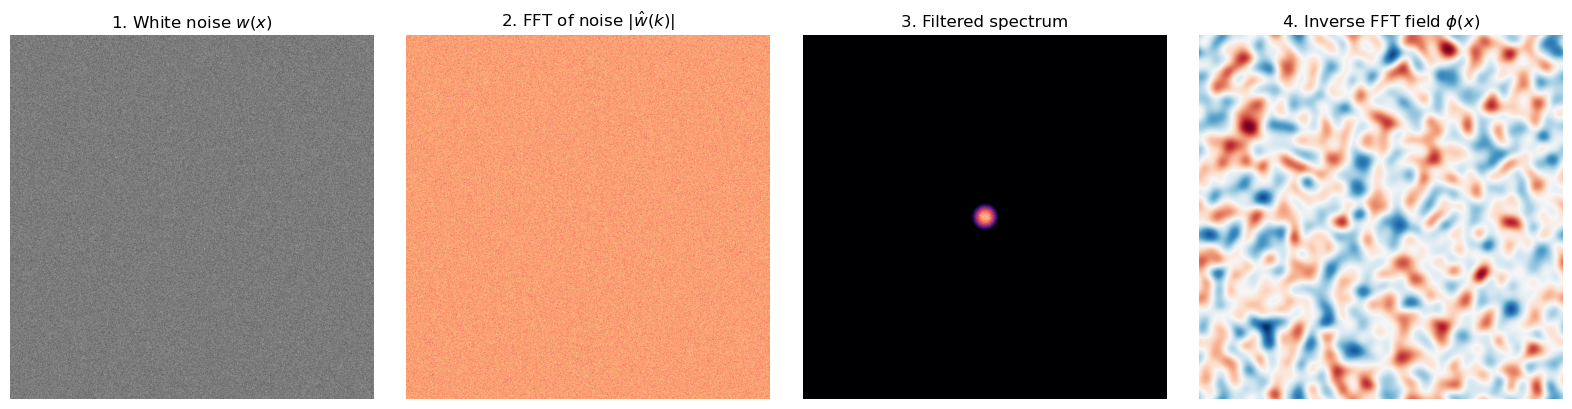
\includegraphics[width=0.8\textwidth]{fig/Gaussian_Random_Field.jpg}
    \caption{Example realization of a Gaussian random field.}
    \label{fig:grf}
\end{figure}

To map $\phi$ into a magnetization-like field $m\in[-1,1]$, one option is
\begin{equation}
m_{i,j}=m_0+(1-|m_0|)\,\tanh\!\Big(\tfrac{\phi_{i,j}}{\tau}\Big),
\end{equation}
where $m_0$ sets the mean magnetization and $\tau$ controls the nonlinearity, with smaller $\tau$ pushing values toward $\pm 1$. Alternatively, a linear clipping scheme may be used. Spins are then sampled independently with
\begin{equation}
\mathbb{P}(\sigma_{i,j}=+1)=\tfrac{1+m_{i,j}}{2},\qquad
\mathbb{P}(\sigma_{i,j}=-1)=\tfrac{1-m_{i,j}}{2},
\end{equation}
yielding an Ising configuration $\sigma\in\{-1,+1\}^{L\times L}$.

The parameter choices have direct impact on structure: the correlation length $\ell$ sets the typical blob size, the global mean $m_0$ fixes magnetization bias, and the field variance or $\tau$ controls contrast. The periodic construction is consistent with the lattice boundary conditions. An equivalent spatial view is to draw white noise $w_{i,j}\sim\mathcal{N}(0,1)$ and convolve with a filter whose Fourier response is $\sqrt{S(\mathbf{k})}$:
\begin{equation}
    \phi \;\stackrel{d}{=}\; \mathcal{F}^{-1}\!\Big[\sqrt{S(\mathbf{k})}\,\mathcal{F}[w]\Big],
\end{equation}
which for Gaussian $S$ corresponds to a Gaussian blur (with periodic wrap) of white noise.

\paragraph{Stochastic Simulation via Gillespie Algorithm.}
The Glauber dynamics can be efficiently simulated using the Gillespie algorithm (\cref{alg:gillespie}), 
which generates statistically exact trajectories of continuous-time Markov processes. 
The procedure is:

\begin{enumerate}
    \item Compute the total flip rate 
    \begin{equation}
        R = \sum_{x} P\big(\sigma(x)\!\to\!-\sigma(x)\big).
    \end{equation}
    \item Draw the next time increment $\Delta t$ from an exponential distribution with mean $1/R$.
    \item Select a site $x$ to flip with probability proportional to its individual rate.
    \item Update $\sigma(x)\mapsto -\sigma(x)$, recompute local fields if needed, and repeat.
\end{enumerate}

\begin{algorithm}[h!]
\caption{Gillespie Simulation of Glauber Dynamics}
\label{alg:gillespie}
\begin{algorithmic}[1]
\State Initialize spin configuration $\sigma$ and compute local fields $h_\gamma(x)$.
\While{simulation time $t < t_{\mathrm{end}}$}
    \State Compute total flip rate 
    \[
        R = \sum_{x} P\big(\sigma(x)\!\to\!-\sigma(x)\big).
    \]
    \State Sample time increment $\Delta t \sim \mathrm{Exp}(R)$.
    \State Select site $x$ with probability 
    \[
        \frac{P(\sigma(x)\!\to\!-\sigma(x))}{R}.
    \]
    \State Flip spin: $\sigma(x) \gets -\sigma(x)$.
    \State Update local fields $h_\gamma(y)$ if needed.
    \State Advance time: $t \gets t + \Delta t$.
\EndWhile
\end{algorithmic}
\end{algorithm}
This algorithm gives an implementation of the Gillespie method for Glauber dynamics, ensuring accurate simulation of the spin system's stochastic behavior.

\paragraph{Stochastic Simulation via $\tau$-leaping Approximation.} The Gillespie algorithm simulates one event at a time, which can be slow for large systems. 
The \emph{$\tau$-leaping} method accelerates the simulation by leaping over a fixed time step $\tau$. 
During this interval, event rates are assumed to be constant. 
The number of events at each site is then sampled from a Poisson distribution. 
This allows many events to be processed in parallel.

\begin{algorithm}[h]
\caption{$\tau$-leaping for Glauber dynamics}
\begin{algorithmic}[1]
\State Initialize spins $s$, time $t=0$
\While{$t < T_{\text{end}}$}
    \State Compute local field $h_{\text{loc}}$
    \State Compute flip rates $r_i = \frac{1}{1 + \exp(2 \beta h_{\text{loc},i} s_i)}$
    \State Choose $\tau = \epsilon / \max_i r_i$
    \State Sample $K_i \sim \mathrm{Poisson}(r_i \tau)$
    \State Update spins: if $K_i$ is odd, flip $s_i$
    \State $t \gets t + \tau$
\EndWhile
\end{algorithmic}
\end{algorithm}

\paragraph{Comparison of Gillespie and $\tau$-leaping} We compare the two methods within a small lattice ($L=128$) to validate the $\tau$-leaping approximation. 
We use the same initial conditions and parameters (temperature $T = 1.0$, coupling strength $J = 1.0$, and external field $h = 0.0$) for both simulations, and for each method, we run 20 independent trials to account for stochastic variability. 
The results are depicted in \cref{fig:gillespie_vs_tau_leaping}. 
The top left panel shows the averaged magnetization over time, while the top right panel displays the free energy evolution. The bottom panels illustrate the error between the two methods in terms of magnetization and free energy. 
The results demonstrate the mean energy and magnetization from both methods are in good agreement, and the varience of $\tau$-leaping is slightly larger than Gillespie. 
These findings confirm that the $\tau$-leaping method is a valid approximation for simulating Glauber dynamics, providing significant computational speedup (see \cref{tab:gillespie_vs_tau_leaping}) while maintaining accuracy with a small sacrifice in variation.
\begin{figure}
    \centering
    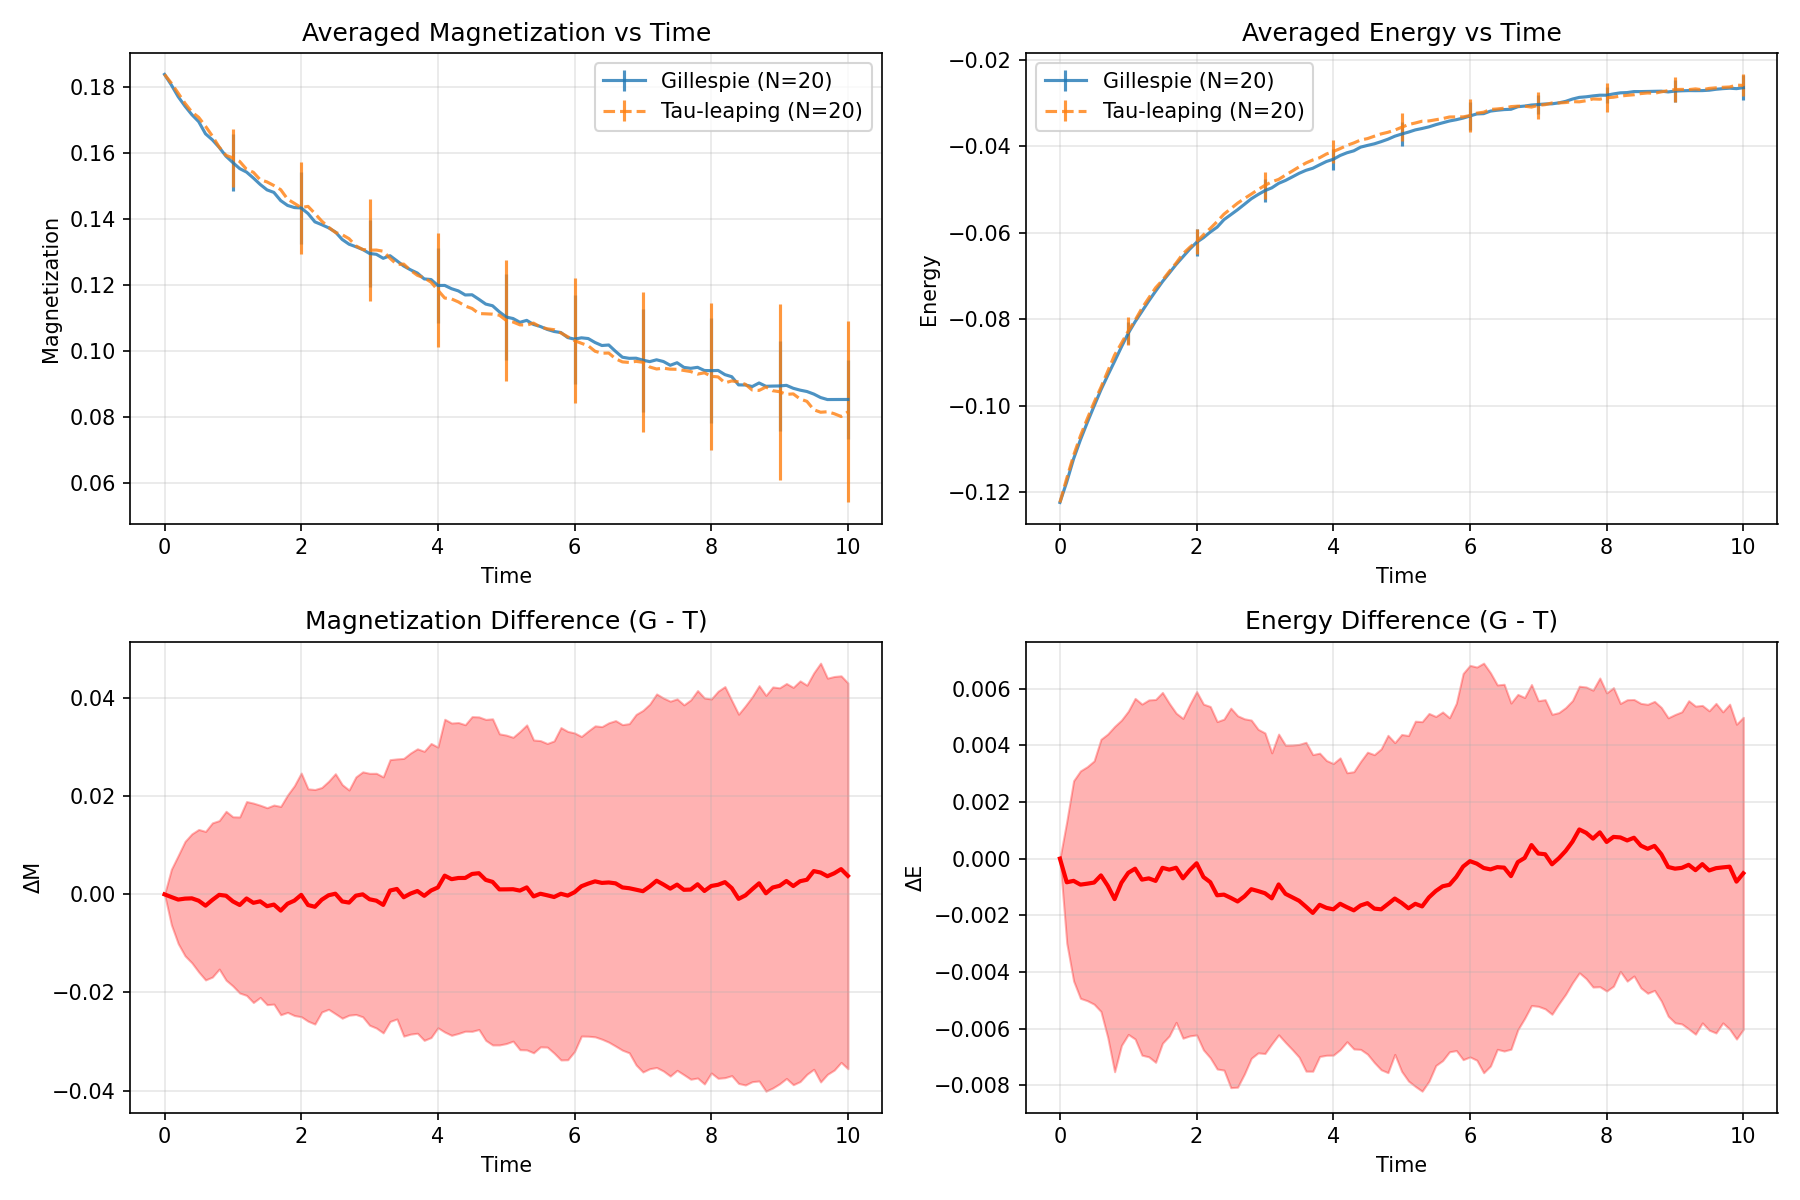
\includegraphics[width=0.8\textwidth]{fig/ising_L128_ell8.0_sigma1.0_tau1.0_m00.2_beta1.0_eps0.02_compare_N20.png}
    \caption{Comparison of Gillespie and $\tau$-leaping methods for simulating Glauber dynamics on a $128 \times 128$ lattice. The top left panel shows the averaged magnization over time and the top right panel shows the free energy evolution over time. The bottom panels show the error between the two methods in terms of magnetization and free energy.}
    \label{fig:gillespie_vs_tau_leaping}
\end{figure}

\begin{table}
    \centering
    \begin{tabular}{ll}
        \hline
        \hline
        Method & Simulation Time of 20 Trails \\
        \hline
        Gillespie & $786.51$s \\
        $\tau$-leaping & $10.79$s \\
        \hline
        \hline
    \end{tabular}
    \caption{Comparison of Gillespie and $\tau$-leaping methods for simulating Glauber dynamics on a $128 \times 128$ lattice. The table shows the final magnetization, free energy, and error for both methods.}
    \label{tab:gillespie_vs_tau_leaping}
\end{table}

\section{PDE}

\subsection{Hydrodynamic Limit for Glauber-Kac}

Starting from the Glauber dynamics introduced in \cref{sec:glauber}, we consider the lattice in $[0,1]^d$. When the lattice size tends to infinity $L\to\infty$, and the empirical magnetization field
\begin{equation}
    m^L(t,\mathbf{x}) = \frac{1}{B^d}\sum_{z\in \Lambda_B(\mathbf{x})} \sigma_t(z)
\end{equation}
is coarse-grained over mesoscopic blocks of size $B$, the law of large numbers implies convergence of $m^L(t,\mathbf{x})$ to a deterministic limit $m(t,\mathbf{x})$. 
In this hydrodynamic limit, the Glauber dynamics is described by the nonlinear nonlocal PDE
\begin{equation}\label{eq:nonlocal}
    \partial_t m(t,\mathbf{x}) \;=\; -\,m(t,\mathbf{x})\;+\;\tanh\!\Big(\beta\, (J_\gamma * m)(t,\mathbf{x}) + \beta h\Big), 
    \qquad m(0,\mathbf{x})=m_0(\mathbf{x}),
\end{equation}
where the convolution operator is defined by
\begin{equation}
    \label{eq:convolution}
    (J_\gamma * m)(\mathbf{x}) \;=\; \int_{\mathbb{T}^d} J_\gamma(\mathbf{x},\mathbf{y})\,m(\mathbf{y})\,d\mathbf{y}.
\end{equation}

Equation~\eqref{eq:nonlocal} is the mesoscopic limit of the Glauber--Kac dynamics: 
the microscopic randomness averages out, and the macroscopic magnetization evolves deterministically according to a nonlocal reaction term given by the Kac potential.

\subsection{From the Nonlocal to the Local PDE}
Assume $m$ is smooth on the scale of $\gamma$, we can perform a Taylor expansion of the convolution term in \cref{eq:convolution}:
\begin{equation}
    (J_\gamma * m)(\mathbf{x}) = m(\mathbf{x}) + \frac{\gamma^2}{2}\Delta m(\mathbf{x}) + O(\gamma^4).
\end{equation}

Also, we can expand $\tanh$ in \cref{eq:nonlocal} around $m(\mathbf{x}) + h$:
\begin{equation}
    \tanh(\beta u) = \beta u - \frac{(\beta u)^3}{3} + O(u^5).
\end{equation}

Substituting these expansions into \cref{eq:nonlocal} and neglecting higher-order terms, we obtain the local reaction-diffusion PDE:
\begin{equation}\label{eq:local}
    \partial_t m(t,\mathbf{x}) = \kappa \Delta m(t,\mathbf{x}) - f(m(t,\mathbf{x})) + \beta h,
    \qquad m(0,\mathbf{x})=m_0(\mathbf{x}),
\end{equation}
where the effective diffusion coefficient is given by
\begin{equation}
    \kappa = \beta \frac{m_2}{2d} \gamma^2,
\end{equation}
with $m_2 = \int_{\mathbb{R}^d} |x|^2 J(x) dx$ being the second moment of the kernel $J$. And the reaction term is
\begin{equation}
    f(m) = -rm - u m^3 + \text{higher order terms}, \quad r = 1-\beta, \quad u = \frac{\beta^3}{3}.
\end{equation} 


\section{Experimental Settings}

\subsection{Parameter Configuration}

Our computational experiments are designed to systematically explore the parameter space of the Ising model and its mesoscopic approximations. The base configuration uses:

\begin{itemize}
    \item \textbf{Coupling strength}: $J = 1.0$ (dimensionless units)
    \item \textbf{Critical temperature}: $T_c = 2.27$ (for 2D square lattice)
    \item \textbf{Lattice size}: $L = 1024$ with coarse-graining to $M = 128$
    \item \textbf{Block size}: $B = 8$ (coarse-graining ratio $L/M = 8$)
    \item \textbf{Spatial resolution}: $\delta = 1/M = 0.0078125$
\end{itemize}

\subsubsection{Temperature Regimes}

We investigate two distinct temperature regimes:

\begin{enumerate}
    \item \textbf{Low temperature} ($T = 1.0$): Below critical temperature, corresponding to the ordered phase where $T/T_c \approx 0.44$
    \item \textbf{High temperature} ($T = 4.0$): Above critical temperature, corresponding to the disordered phase where $T/T_c \approx 1.76$
\end{enumerate}

\subsubsection{External Field Variations}

The external magnetic field $h$ is varied across four values to study its effect on the system dynamics:

\begin{itemize}
    \item $h = 0.0$ (no external field)
    % \item $h = 0.5$ (weak external field)
    \item $h = 1.0$ (moderate external field)
    % \item $h = 2.0$ (strong external field)
\end{itemize}

\subsubsection{Kernel Range Studies}

To investigate the role of interaction range in nonlocal dynamics, we vary the kernel domain size:

\begin{itemize}
    \item \textbf{Local interactions}: $\gamma \to 0$ (nearest-neighbor only)
    \item \textbf{Short-range nonlocal}: $\gamma = 2\delta$ (extended local interactions)
    \item \textbf{Medium-range nonlocal}: $\gamma = 4\delta$ (moderate nonlocal interactions)
\end{itemize}

This systematic variation allows us to study the transition from local to nonlocal behavior and its impact on pattern formation and dynamics.

This computational framework will provide insights into:

\begin{itemize}
    \item The relationship between microscopic and macroscopic dynamics
    \item The validity of continuum approximations
    \item The role of nonlocal interactions in pattern formation
    \item Machine learning approaches for complex dynamics
\end{itemize}

\subsection{Data v.s. PDE Solutions}
We compare the original data generated by \Cref{alg:gillespie} and PDE solutions under different settings.
\begin{table}[h]
    \centering
    \begin{tabular}{lllll}
        \hline
        \hline
        \textbf{External field $h$} & \textbf{Temperature $T$} & \textbf{Kernel parameter $\gamma$} & \textbf{Lattice size $L$} & \textbf{Results} \\
        \hline
        0 & 1 & 0.015625 & 1024 & \Cref{fig:pde_comparison_h0_T1_eps0.015625} \\
        0 & 4 & 0.015625 & 1024 & \Cref{fig:pde_comparison_h0_T4_eps0.015625} \\
        1 & 1 & 0.015625 & 1024 & \Cref{fig:pde_comparison_h1_T1_eps0.015625} \\
        1 & 4 & 0.015625 & 1024 & \Cref{fig:pde_comparison_h1_T4_eps0.015625} \\
        0 & 1 & 0.03125  & 1024 & \Cref{fig:pde_comparison_h0_T1_eps0.03125}  \\
        0 & 4 & 0.03125  & 1024 & \Cref{fig:pde_comparison_h0_T4_eps0.03125}  \\
        1 & 1 & 0.03125  & 1024 & \Cref{fig:pde_comparison_h1_T1_eps0.03125}  \\
        1 & 4 & 0.03125  & 1024 & \Cref{fig:pde_comparison_h1_T4_eps0.03125}  \\
        0 & 1 & 0.015625 & 1024 & \Cref{fig:pde_comparison_h0_T1_eps0.015625} \\
        0 & 4 & 0.015625 & 2048 & \Cref{fig:pde_comparison_h0_T4_eps0.015625_L2048} \\
        1 & 1 & 0.015625 & 2048 & \Cref{fig:pde_comparison_h1_T1_eps0.015625_L2048} \\
        1 & 4 & 0.015625 & 2048 & \Cref{fig:pde_comparison_h1_T4_eps0.015625_L2048} \\
        0 & 1 & 0.03125  & 2048 & \Cref{fig:pde_comparison_h0_T1_eps0.03125_L2048}  \\
        0 & 4 & 0.03125  & 2048 & \Cref{fig:pde_comparison_h0_T4_eps0.03125_L2048}  \\
        1 & 1 & 0.03125  & 2048 & \Cref{fig:pde_comparison_h1_T1_eps0.03125_L2048}  \\
        1 & 4 & 0.03125  & 2048 & \Cref{fig:pde_comparison_h1_T4_eps0.03125_L2048}  \\
        \hline
        \hline
    \end{tabular}
    \caption{Comparison of original data and PDE solutions under different external field $h$, temperature $T$, and kernel parameter $\epsilon$.}
    \label{tab:pde_comparison}
\end{table}

We present the results in \Cref{tab:pde_comparison}. The arrangement of the figure follows a $3 \times 4$ grid layout to clearly compare the original data and the PDE solutions.  


% with epsilon = 0.015625

\begin{figure}[!h]
    \centering
    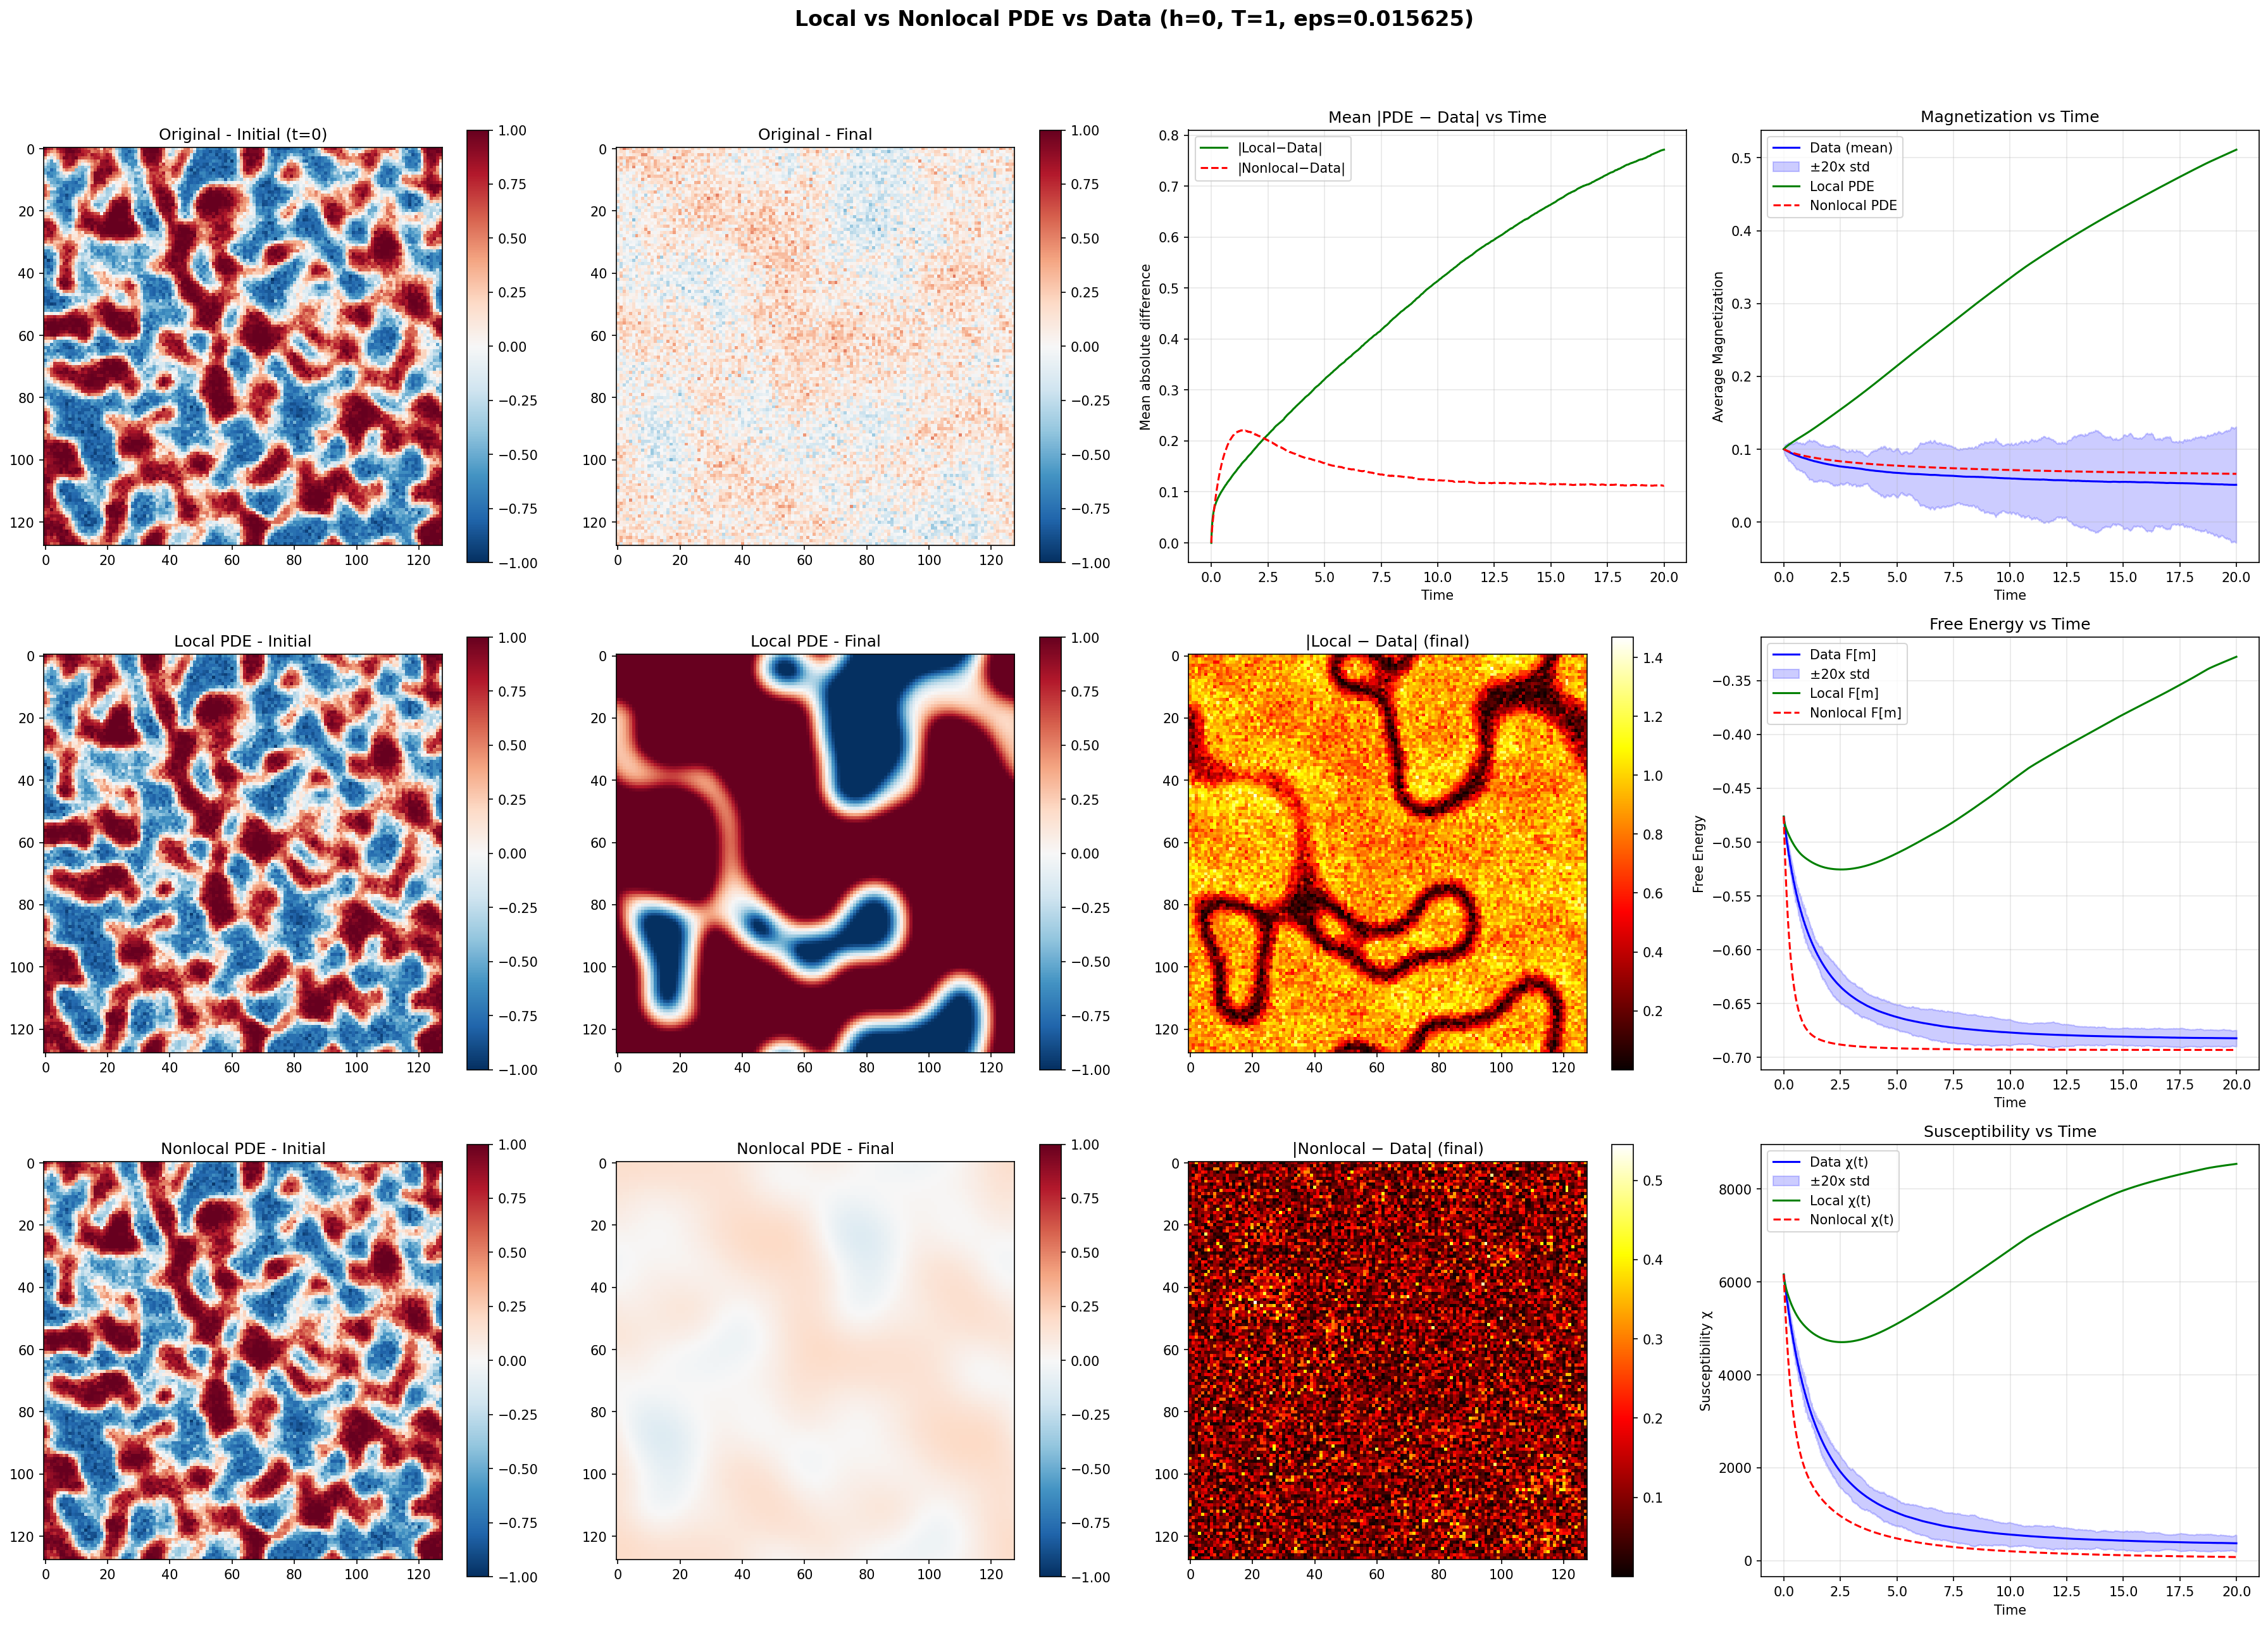
\includegraphics[width=1.0\textwidth]{fig/compare_local_nonlocal_L1024_h0_T1_eps0.015625.png}
    \caption{Comparison of original data and PDE solutions for $h=0$, $T=1$, $\epsilon=0.015625$, $L=1024$.}
    \label{fig:pde_comparison_h0_T1_eps0.015625}
\end{figure}


\begin{figure}[!h]
    \centering
    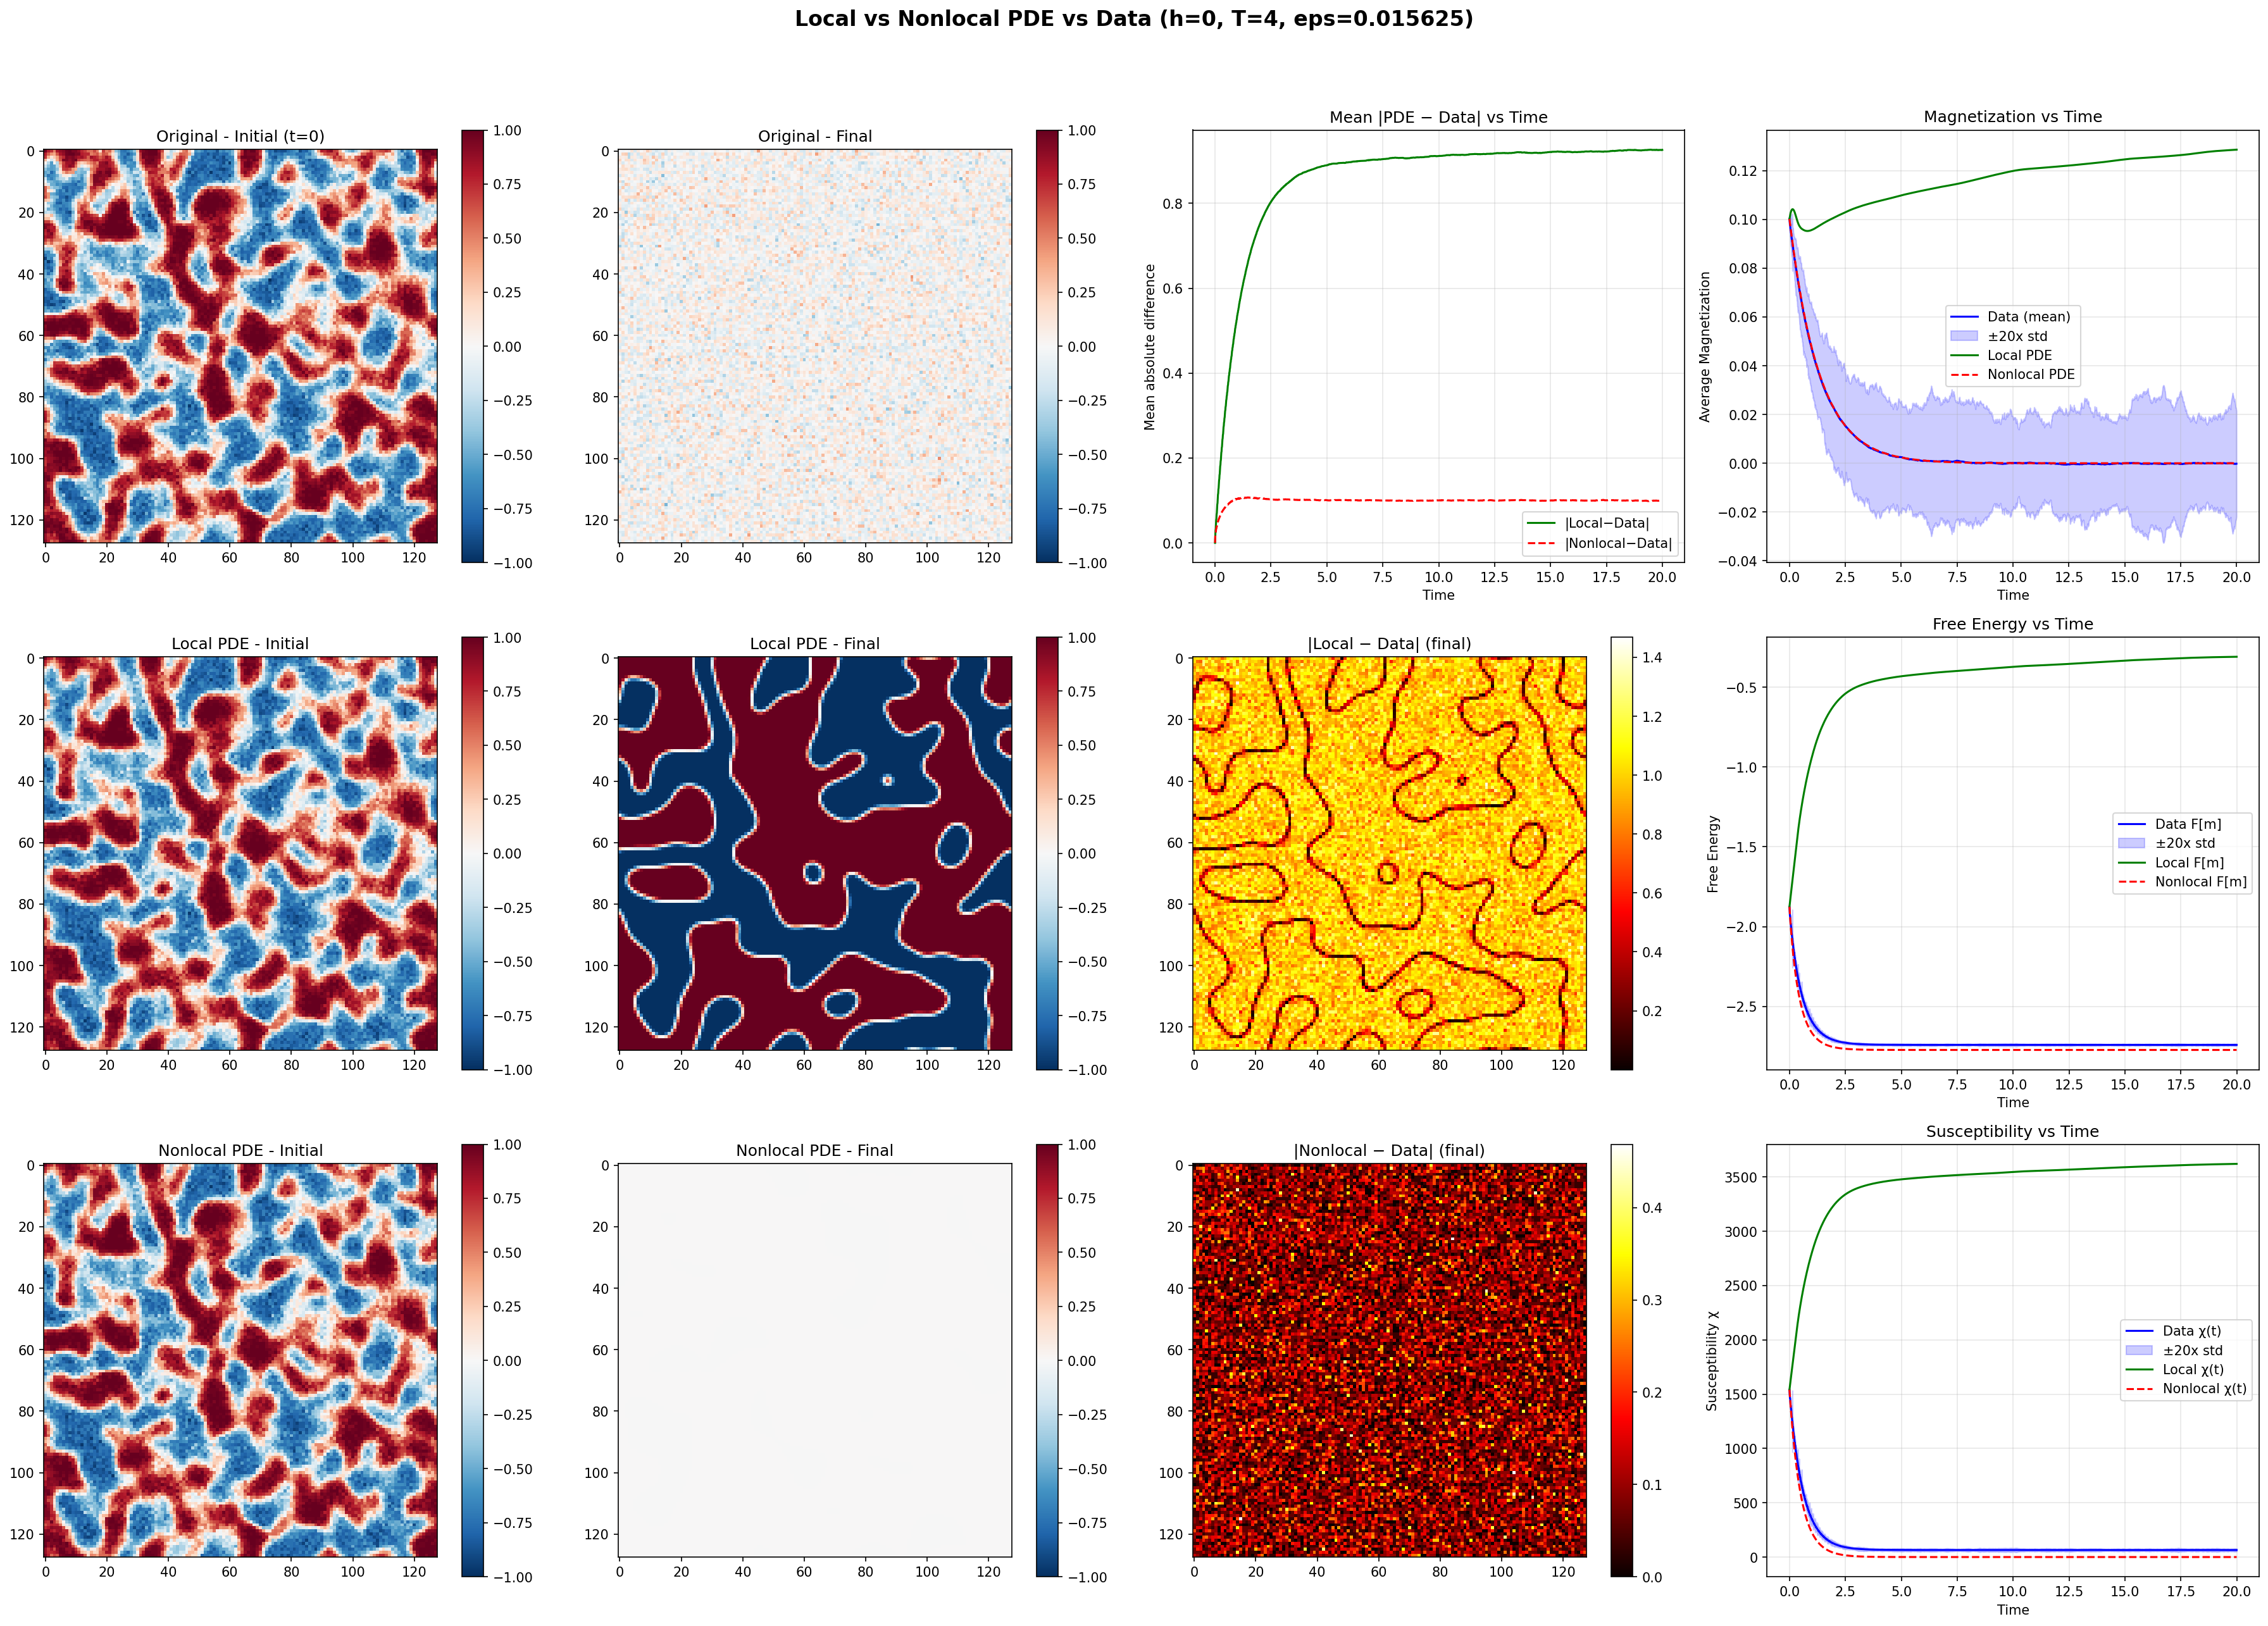
\includegraphics[width=1.0\textwidth]{fig/compare_local_nonlocal_L1024_h0_T4_eps0.015625.png}
    \caption{Comparison of original data and PDE solutions for $h=0$, $T=4$, $\epsilon=0.015625$, $L=1024$.}
    \label{fig:pde_comparison_h0_T4_eps0.015625}
\end{figure}


\begin{figure}[!h]
    \centering
    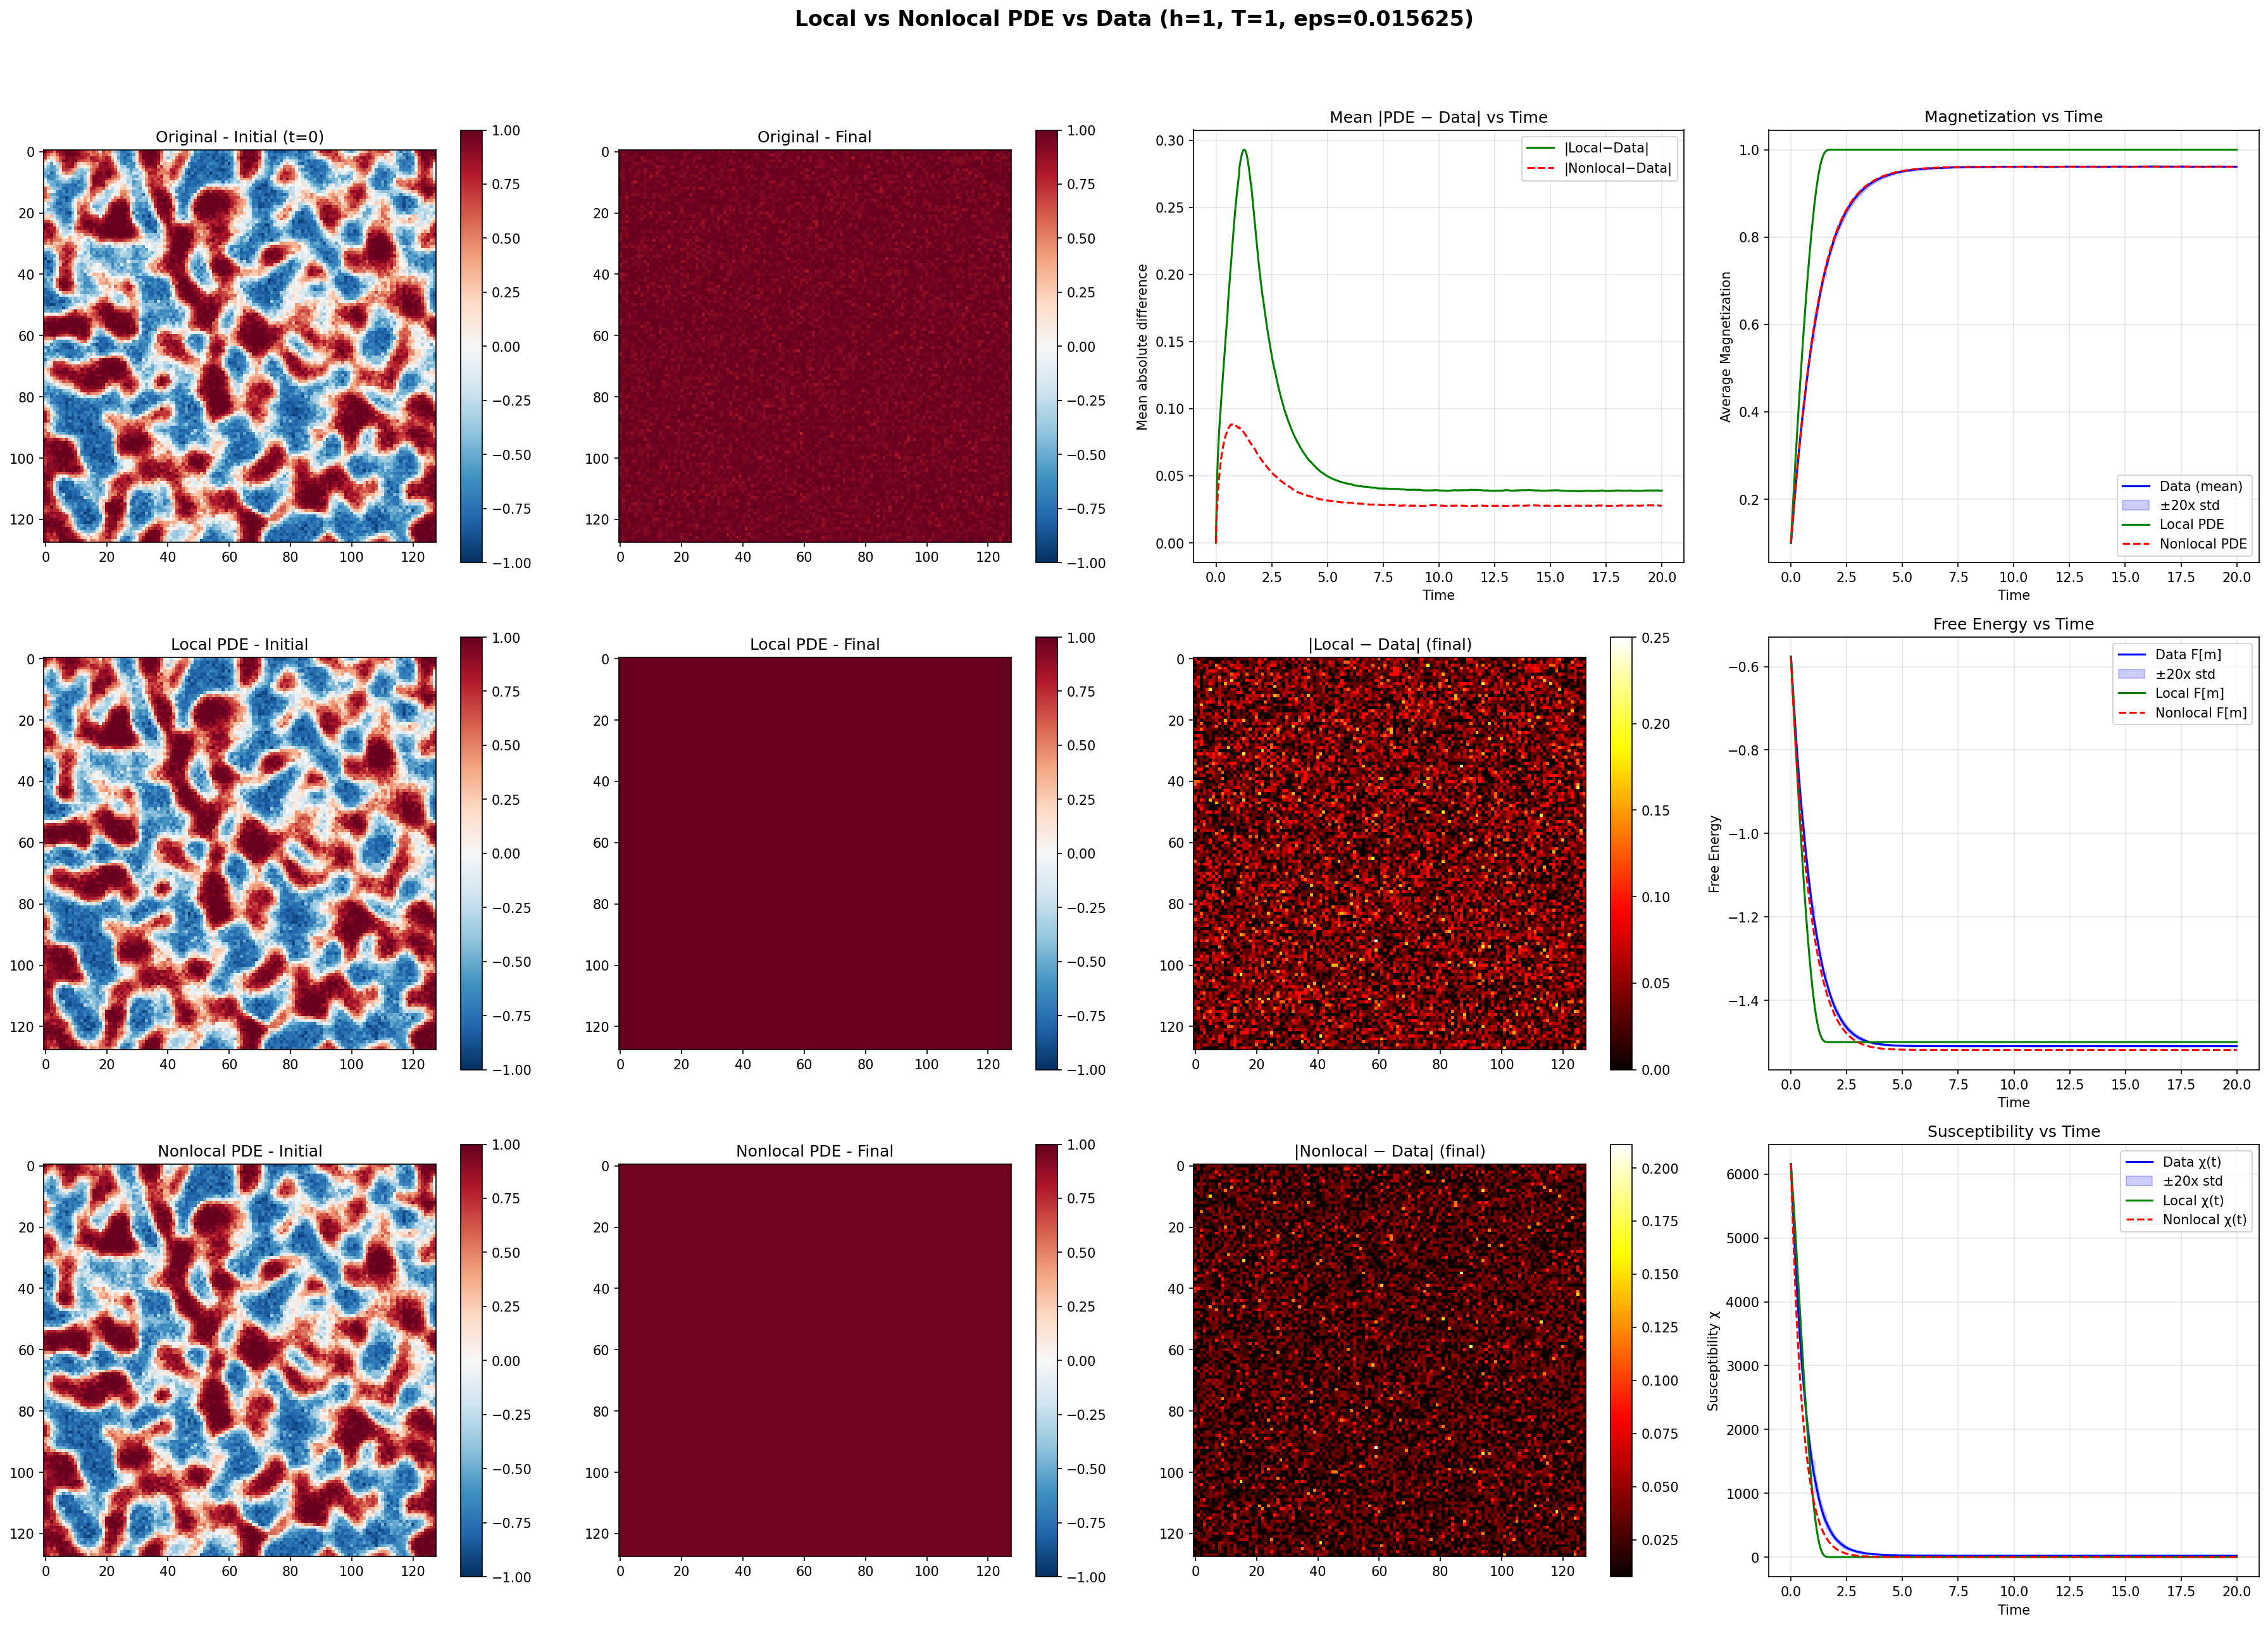
\includegraphics[width=1.0\textwidth]{fig/compare_local_nonlocal_L1024_h1_T1_eps0.015625.png}
    \caption{Comparison of original data and PDE solutions for $h=1$, $T=1$, $\epsilon=0.015625$, $L=1024$.}
    \label{fig:pde_comparison_h1_T1_eps0.015625}
\end{figure}


\begin{figure}[!h]
    \centering
    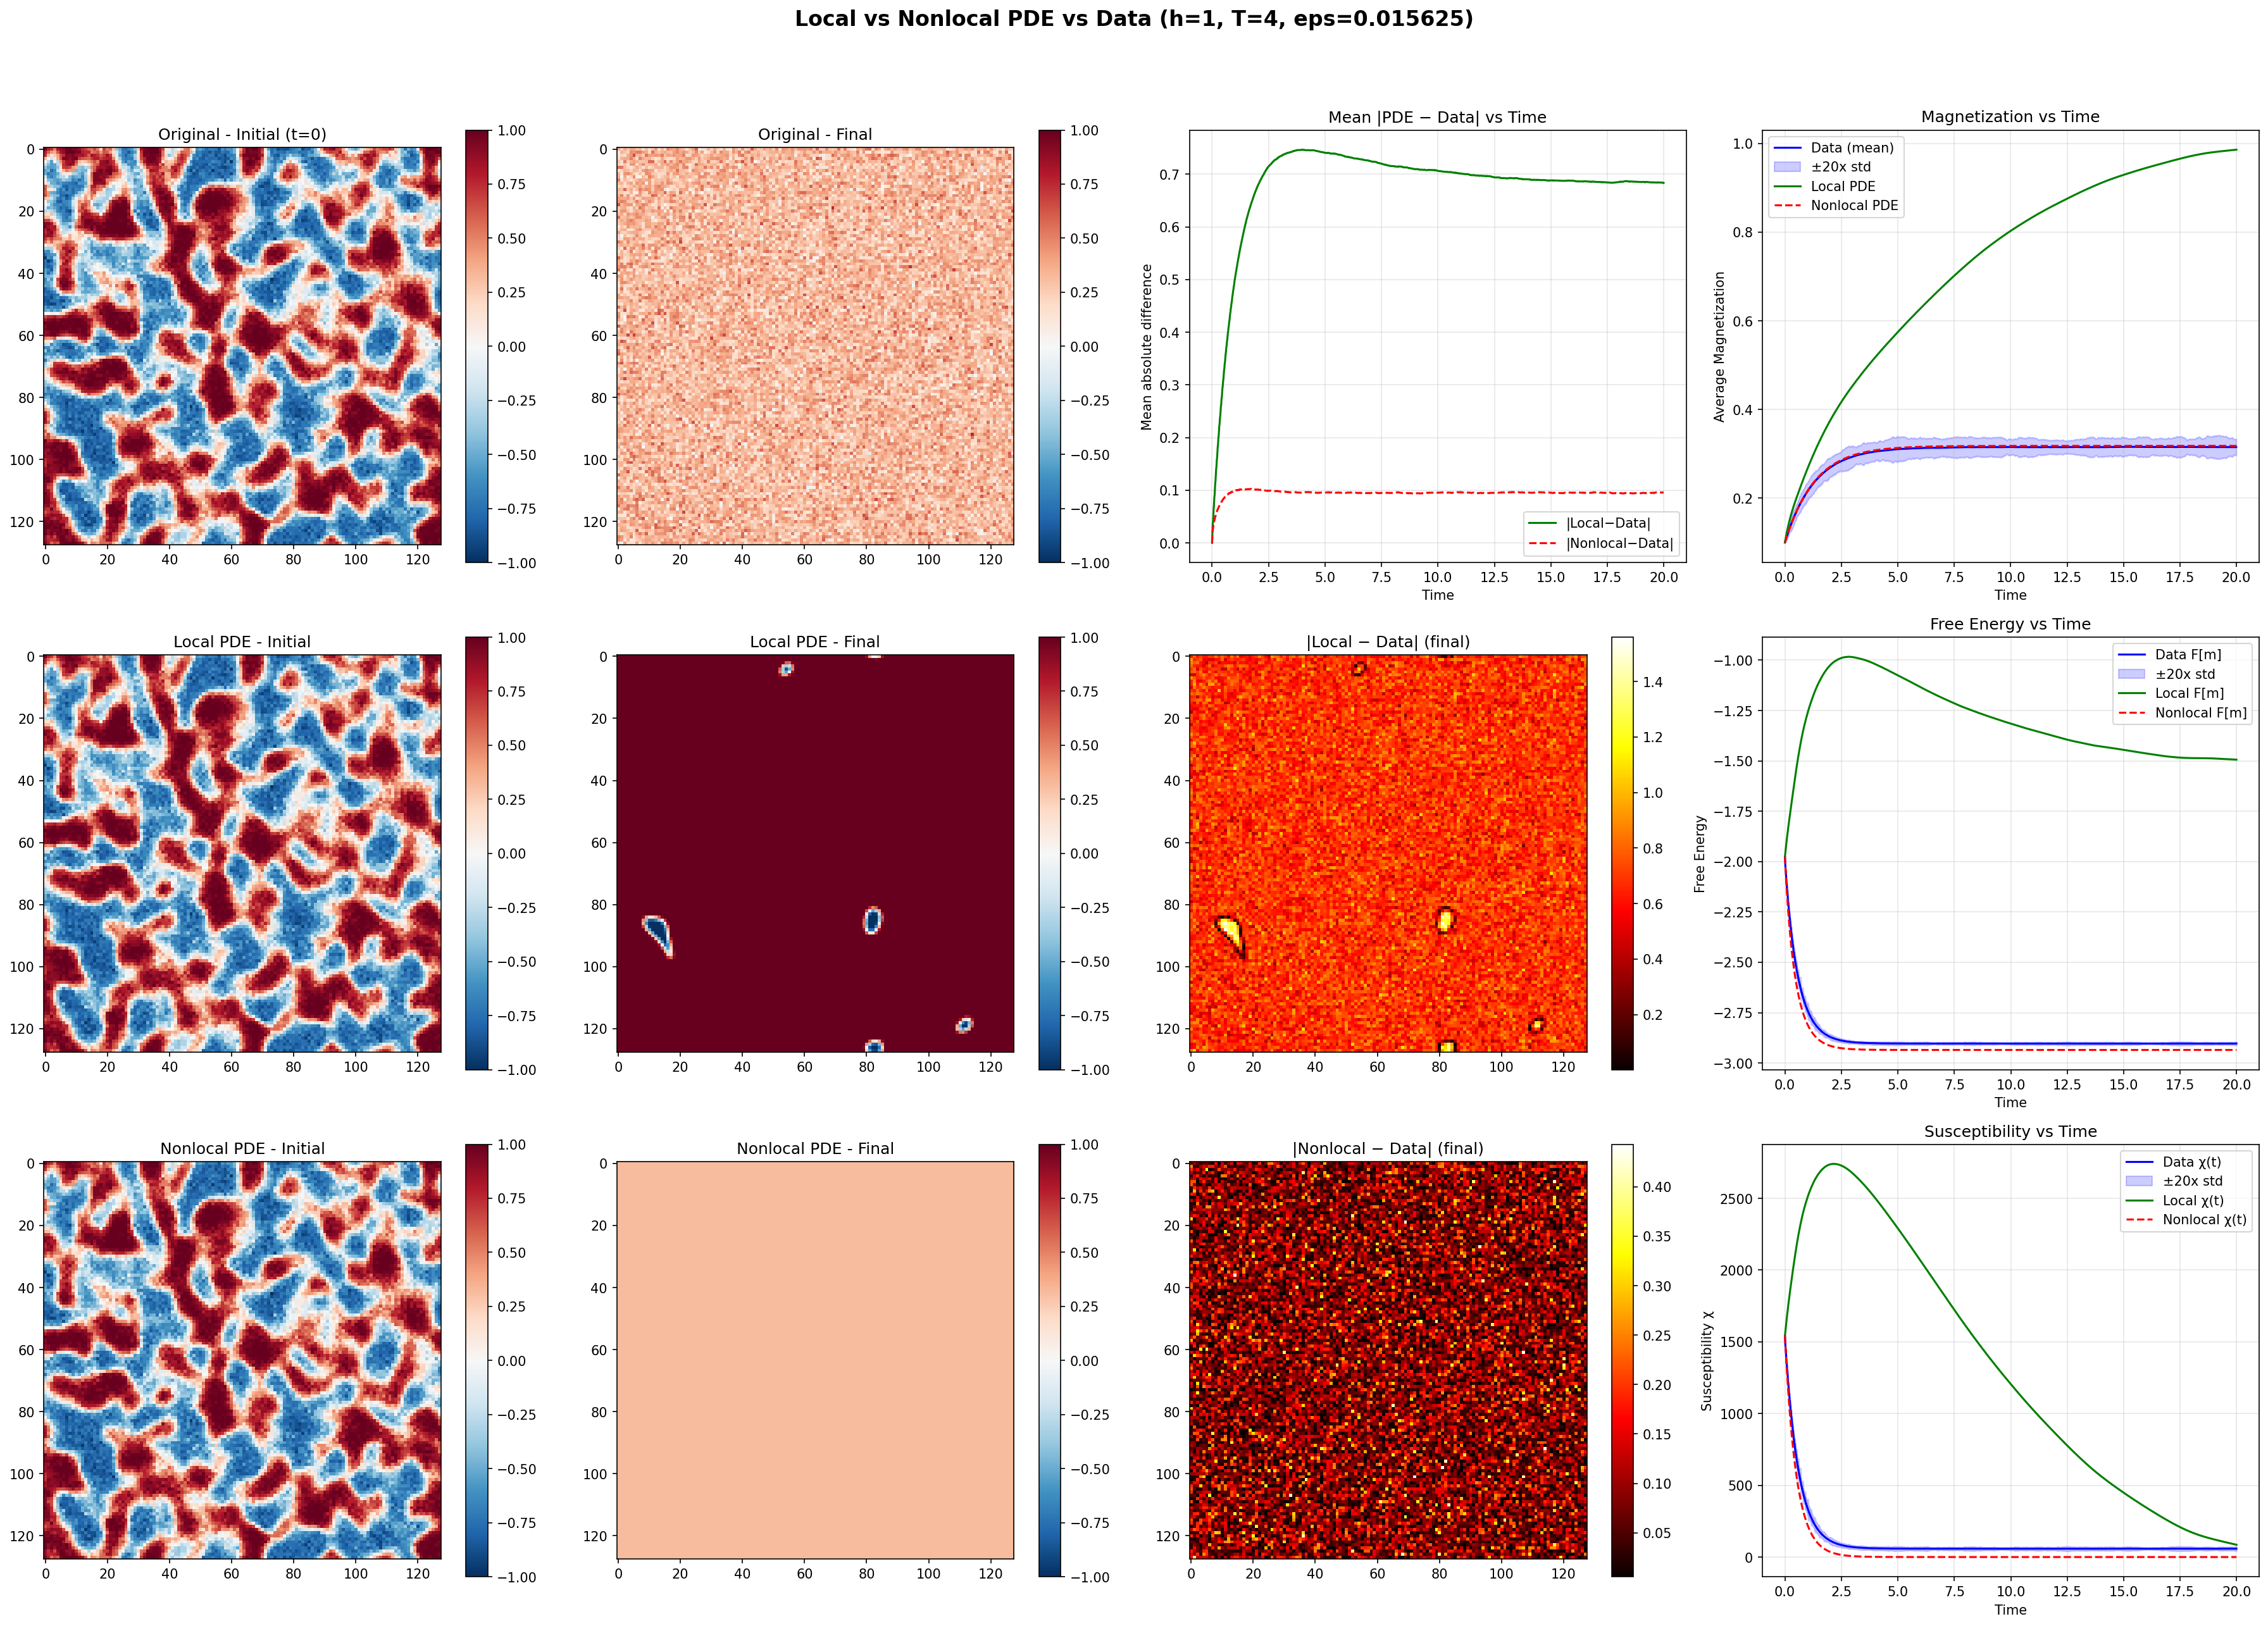
\includegraphics[width=1.0\textwidth]{fig/compare_local_nonlocal_L1024_h1_T4_eps0.015625.png}
    \caption{Comparison of original data and PDE solutions for $h=1$, $T=4$, $\epsilon=0.015625$, $L=1024$.}
    \label{fig:pde_comparison_h1_T4_eps0.015625}
\end{figure}

% with epsilon = 0.03125

\begin{figure}[!h]
    \centering
    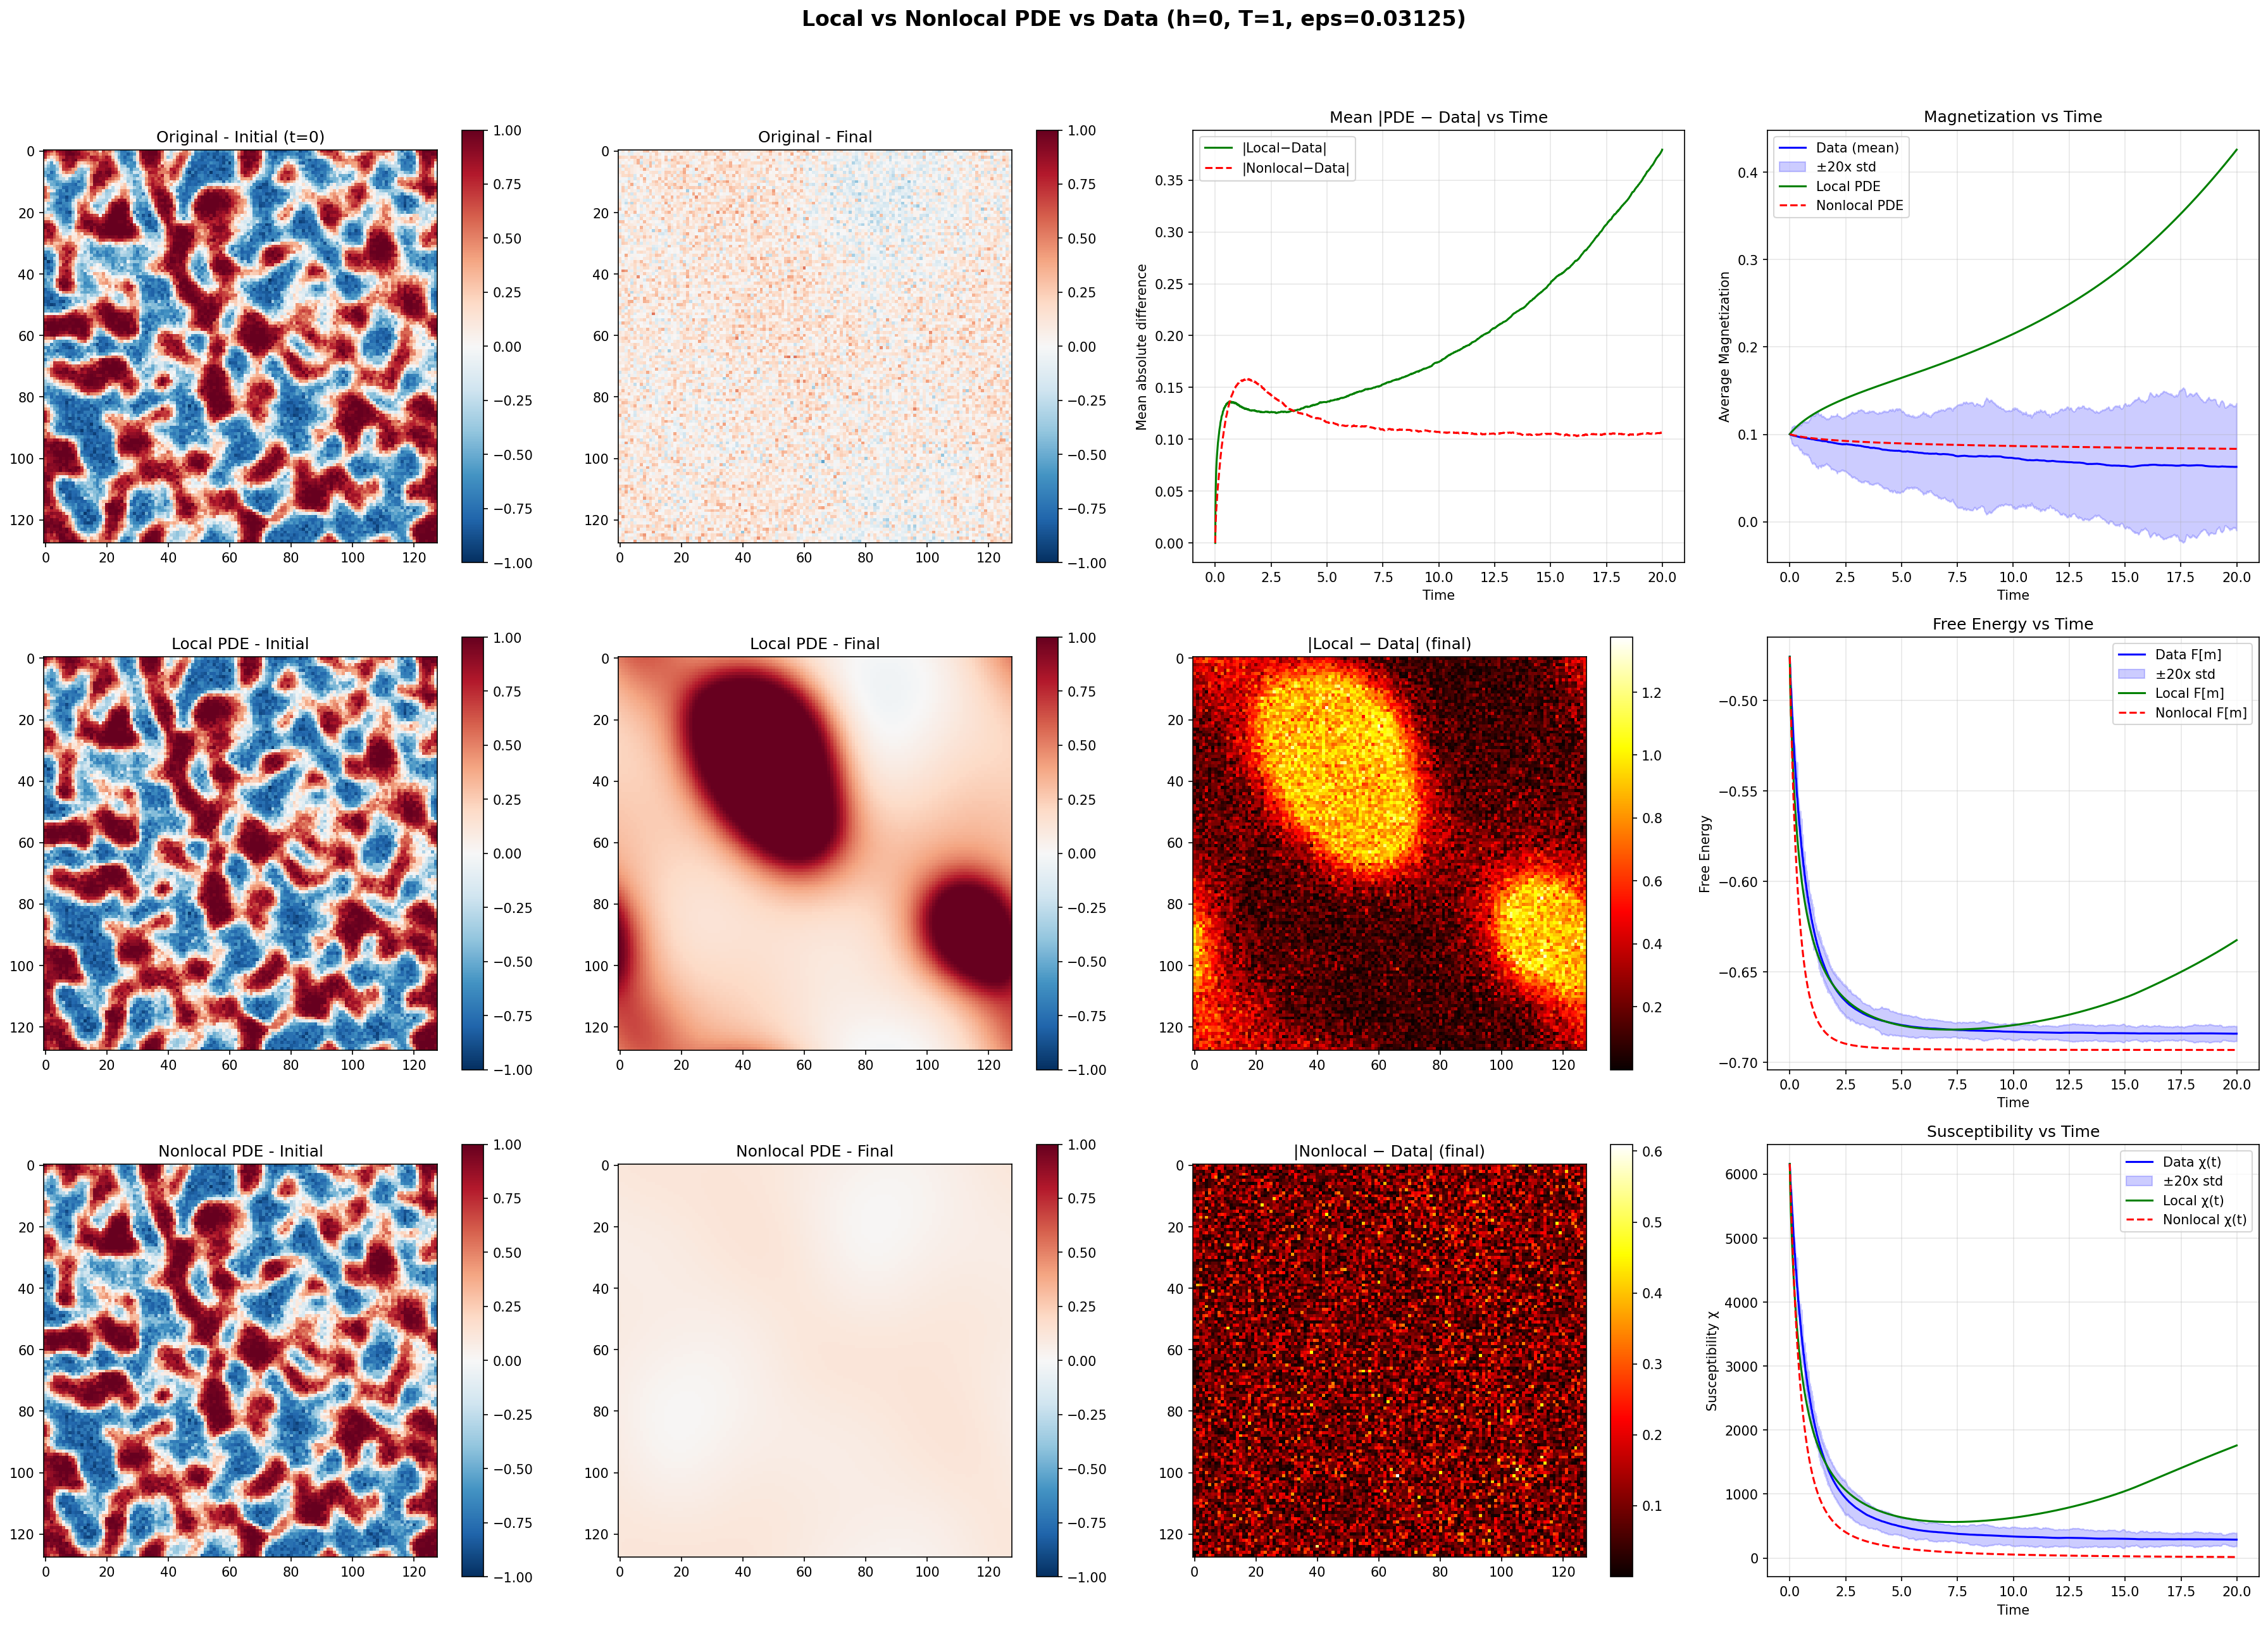
\includegraphics[width=1.0\textwidth]{fig/compare_local_nonlocal_L1024_h0_T1_eps0.03125.png}
    \caption{Comparison of original data and PDE solutions for $h=0$, $T=1$, $\epsilon=0.03125$, $L=1024$.}
    \label{fig:pde_comparison_h0_T1_eps0.03125}
\end{figure}


\begin{figure}[h]
    \centering
    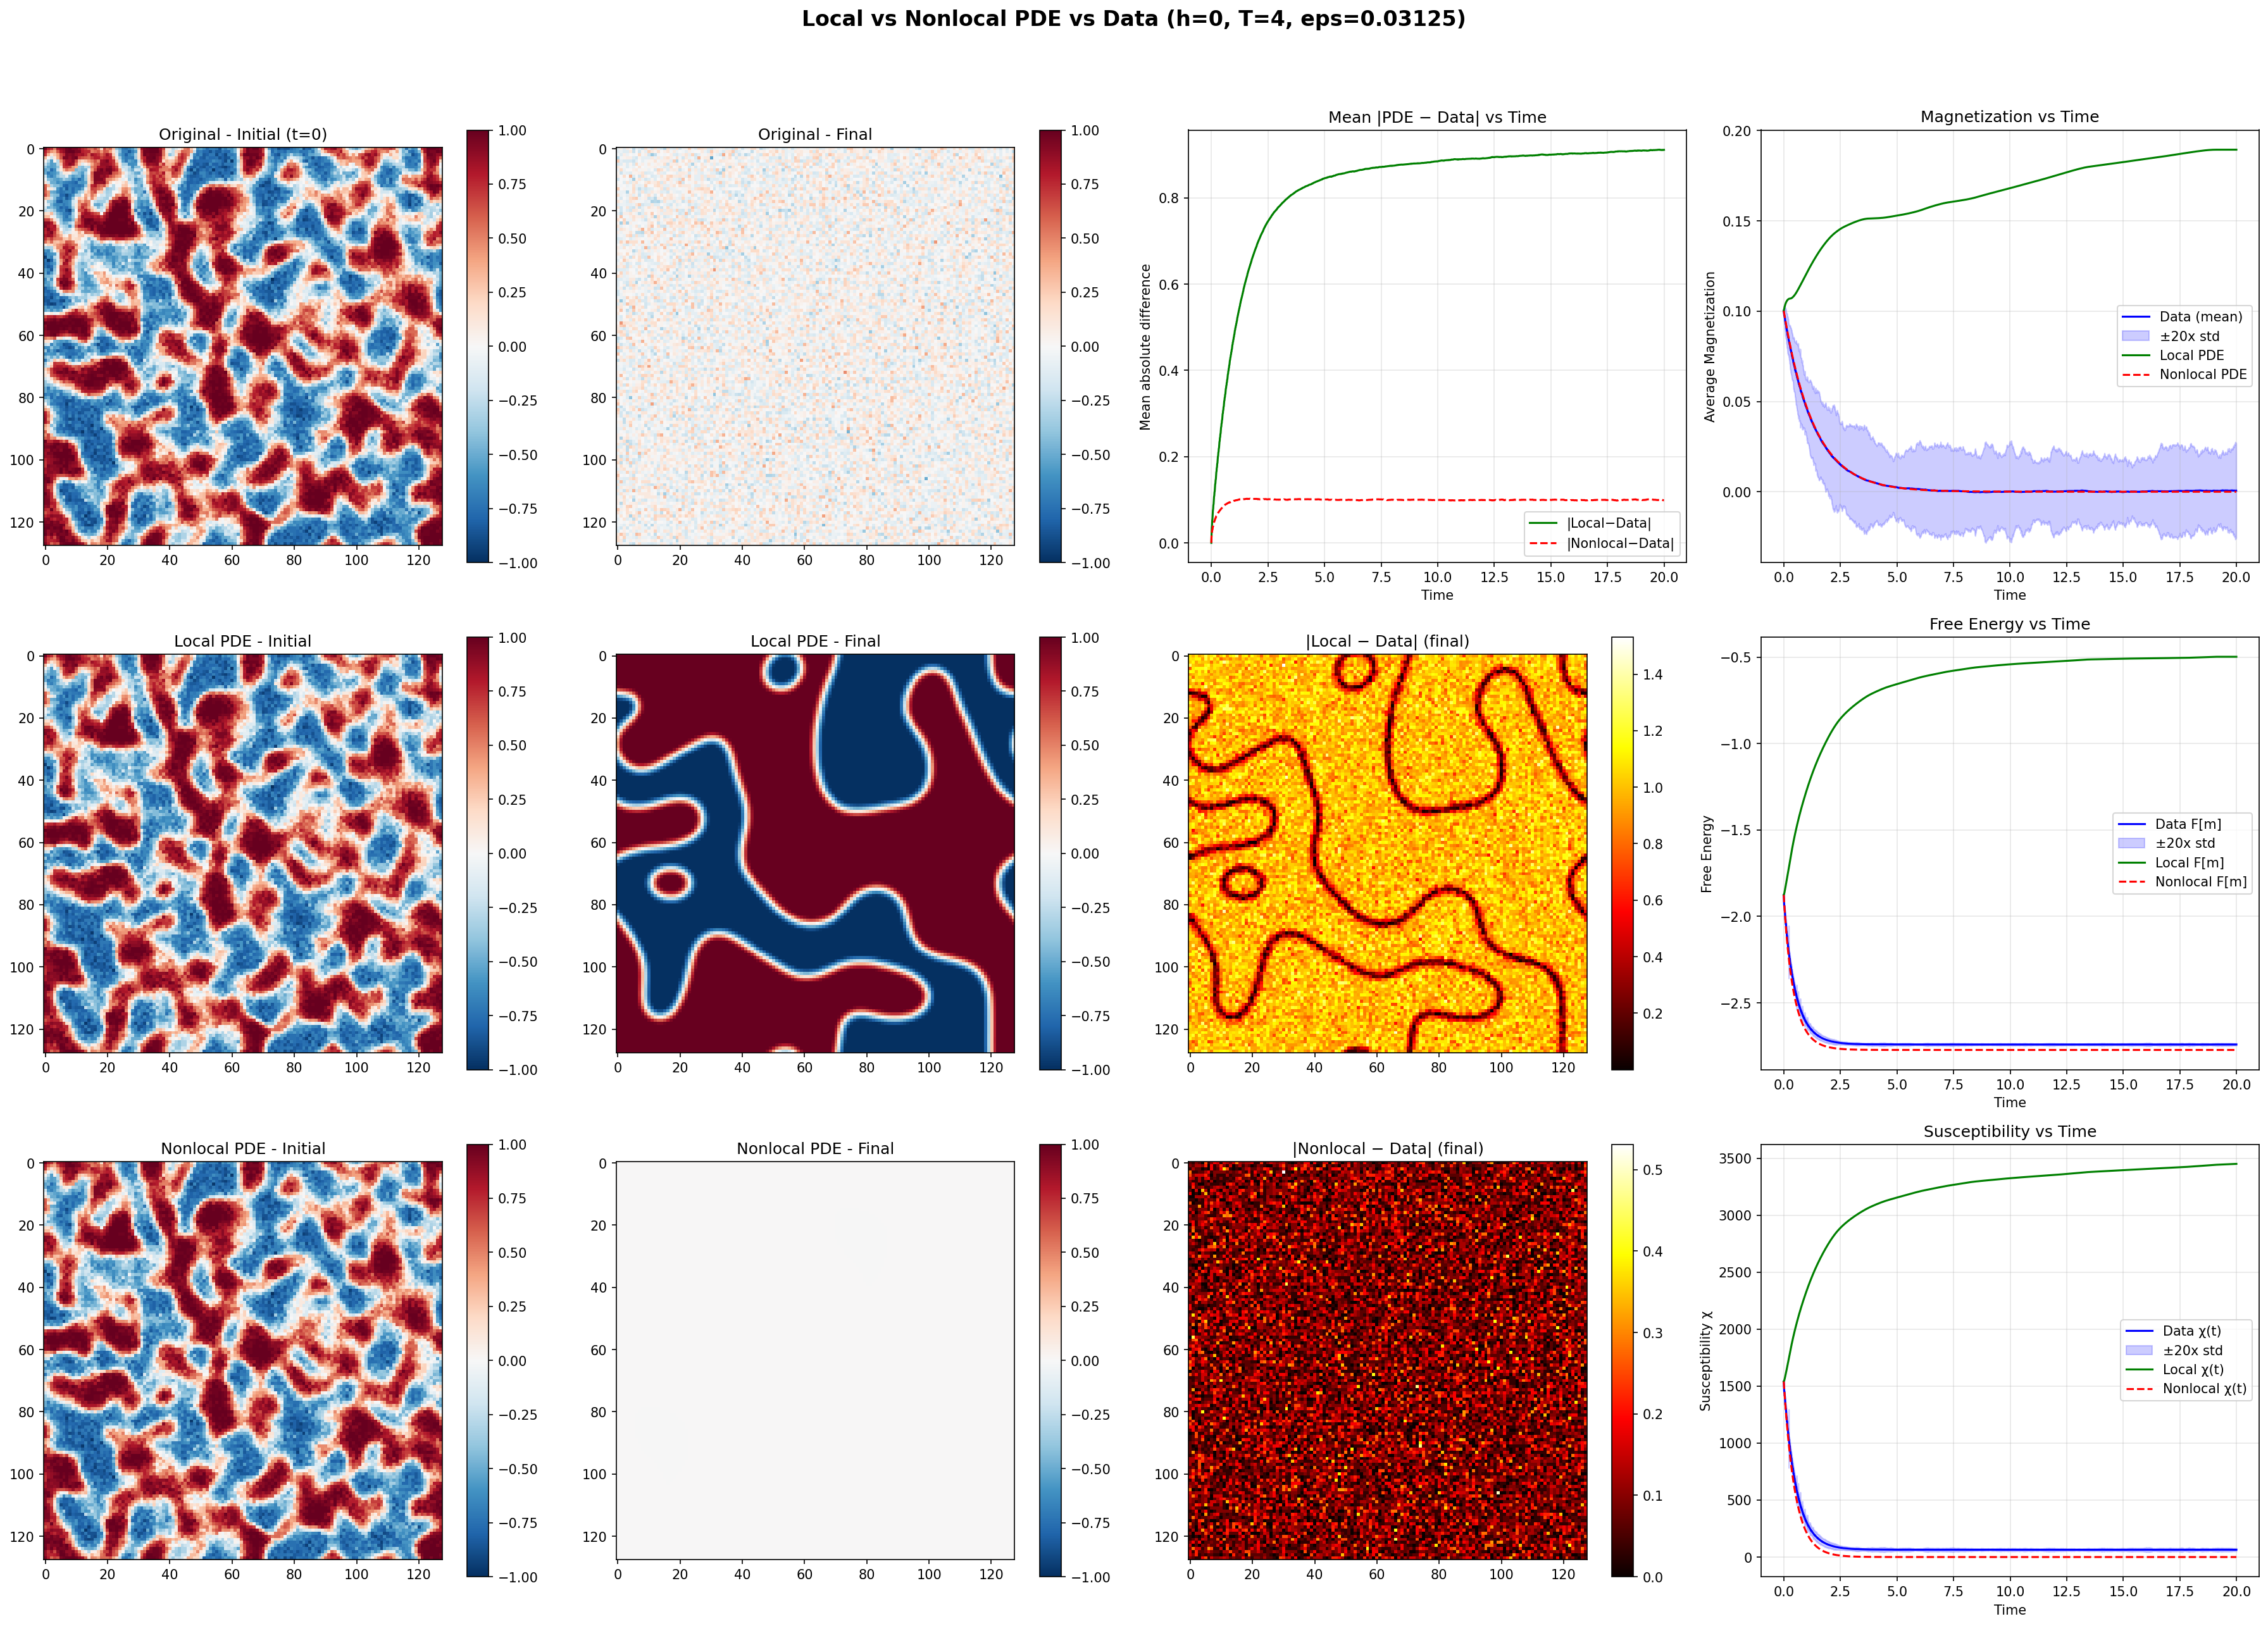
\includegraphics[width=1.0\textwidth]{fig/compare_local_nonlocal_L1024_h0_T4_eps0.03125.png}
    \caption{Comparison of original data and PDE solutions for $h=0$, $T=4$, $\epsilon=0.03125$, $L=1024$.}
    \label{fig:pde_comparison_h0_T4_eps0.03125}
\end{figure}


\begin{figure}[!h]
    \centering
    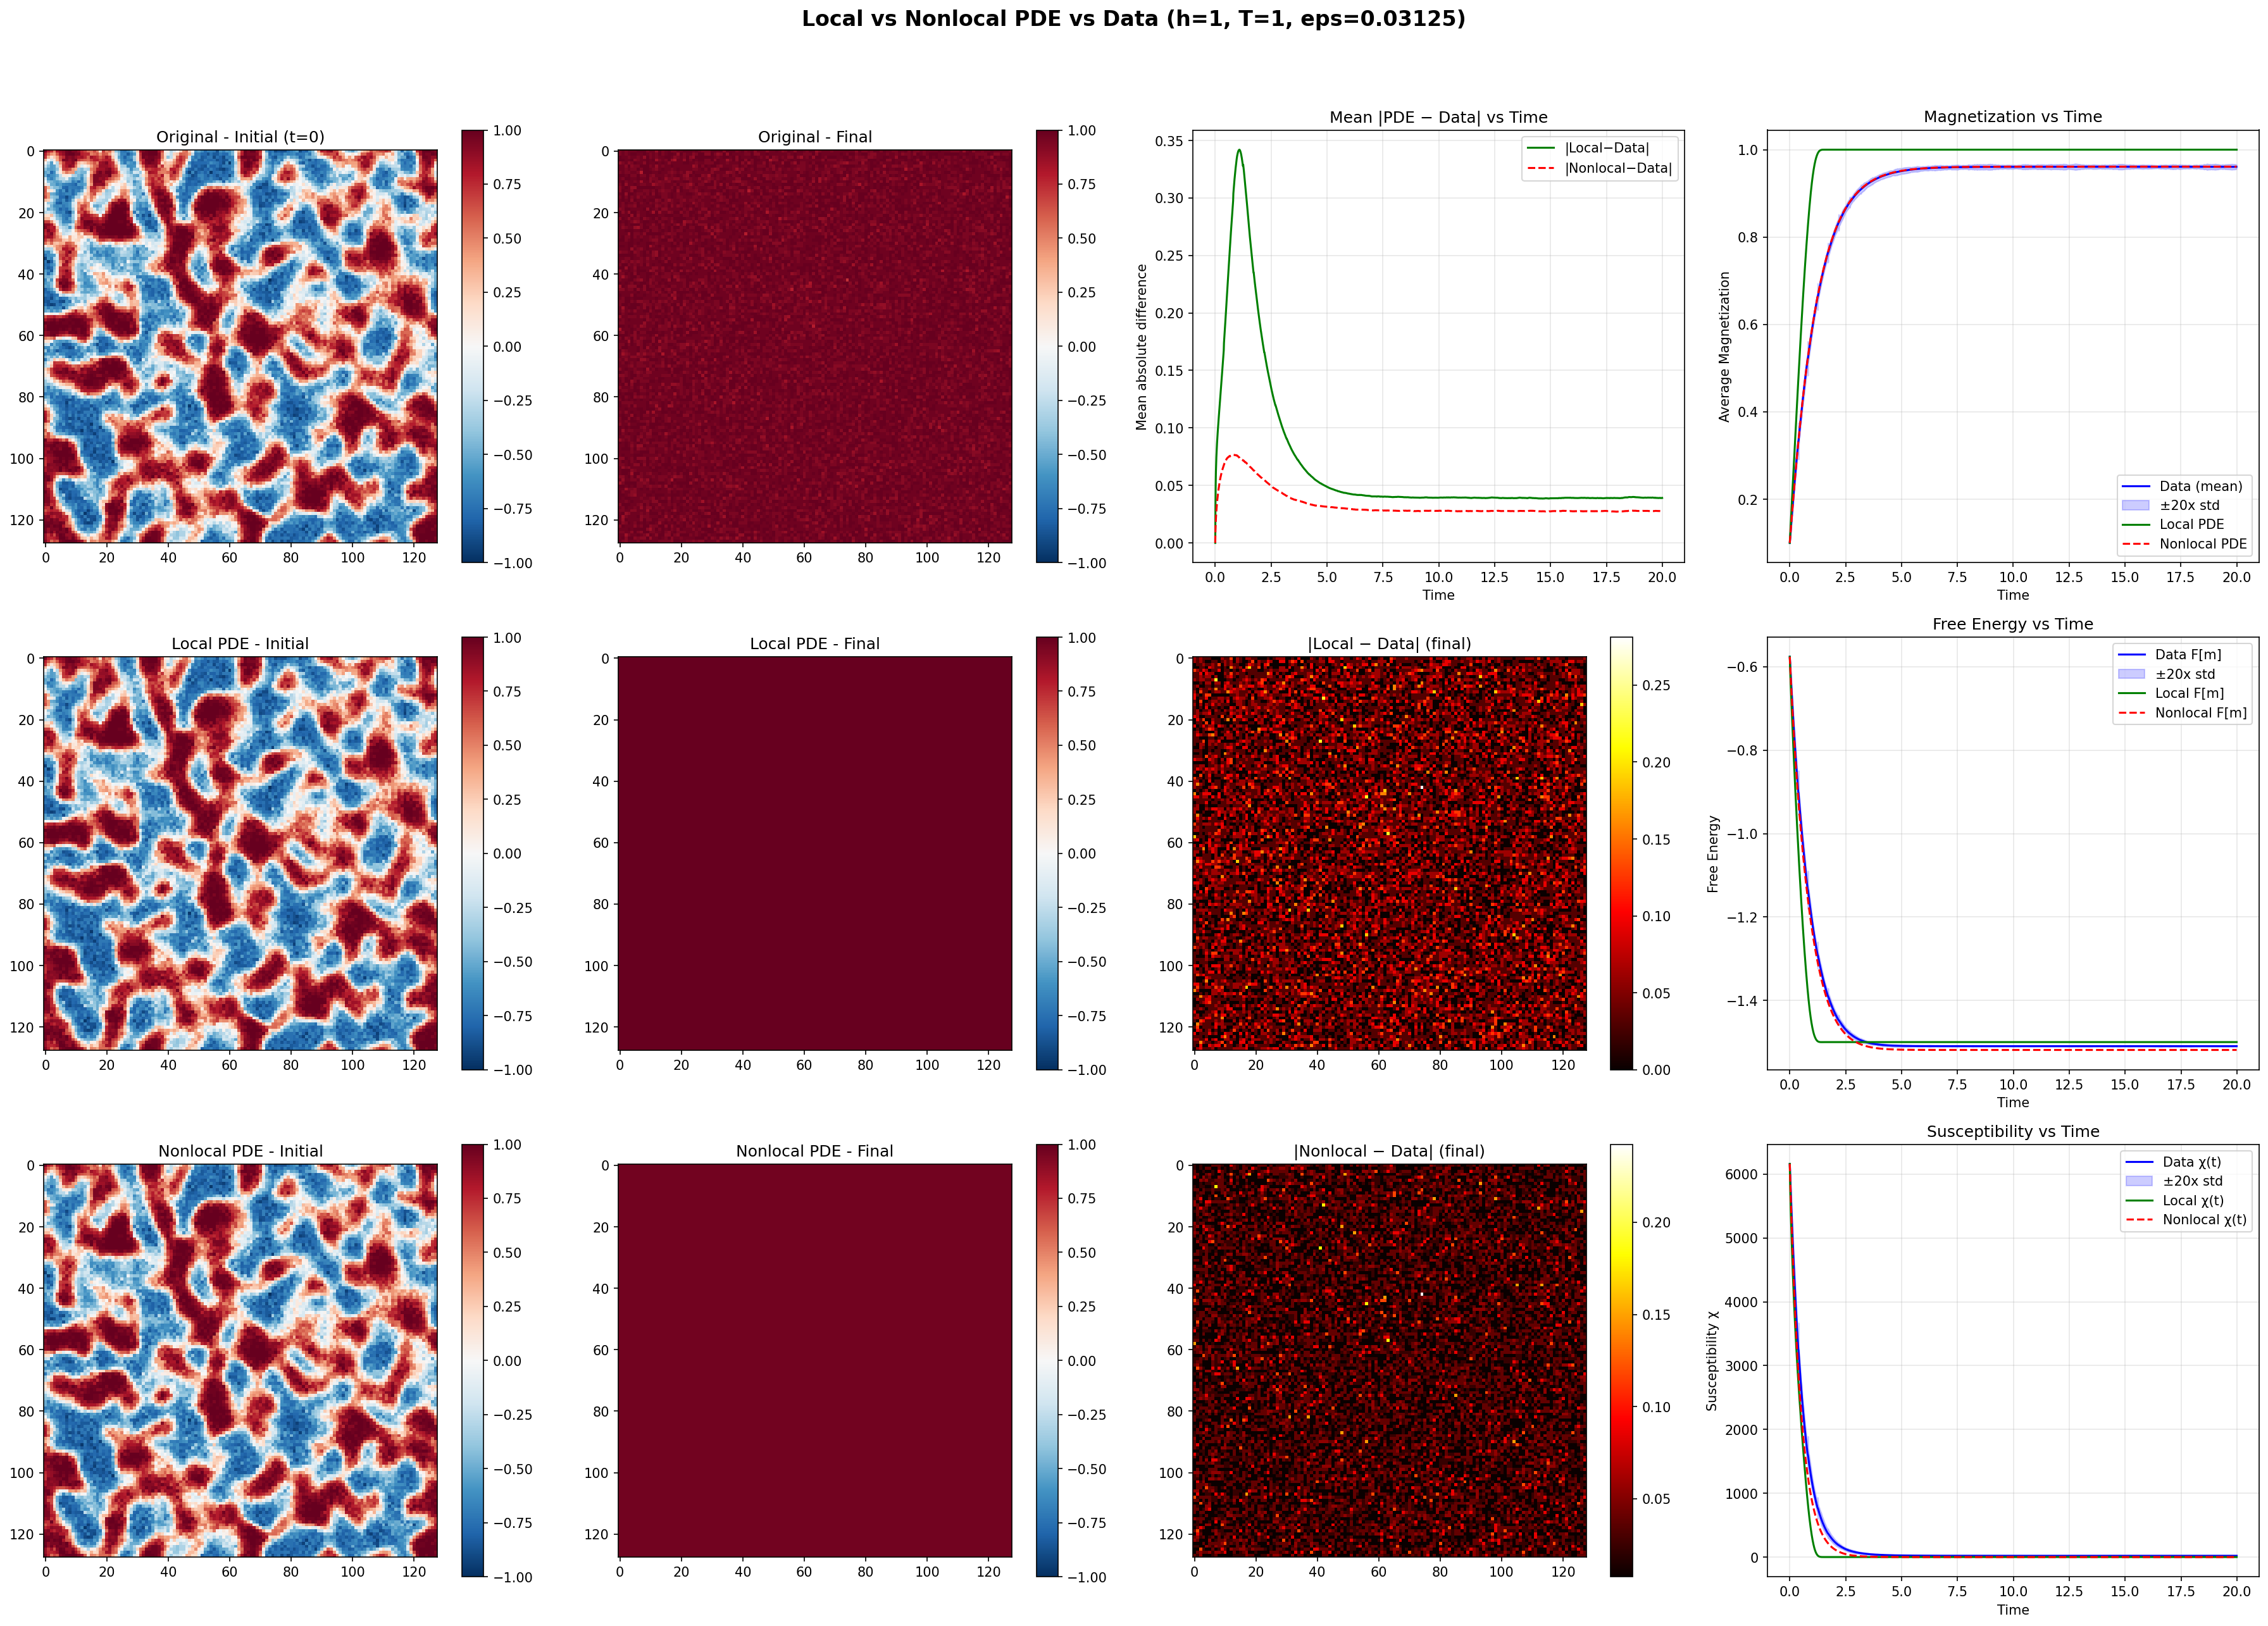
\includegraphics[width=1.0\textwidth]{fig/compare_local_nonlocal_L1024_h1_T1_eps0.03125.png}
    \caption{Comparison of original data and PDE solutions for $h=1$, $T=1$, $\epsilon=0.03125$, $L=1024$.}
    \label{fig:pde_comparison_h1_T1_eps0.03125}
\end{figure}


\begin{figure}[h]
    \centering
    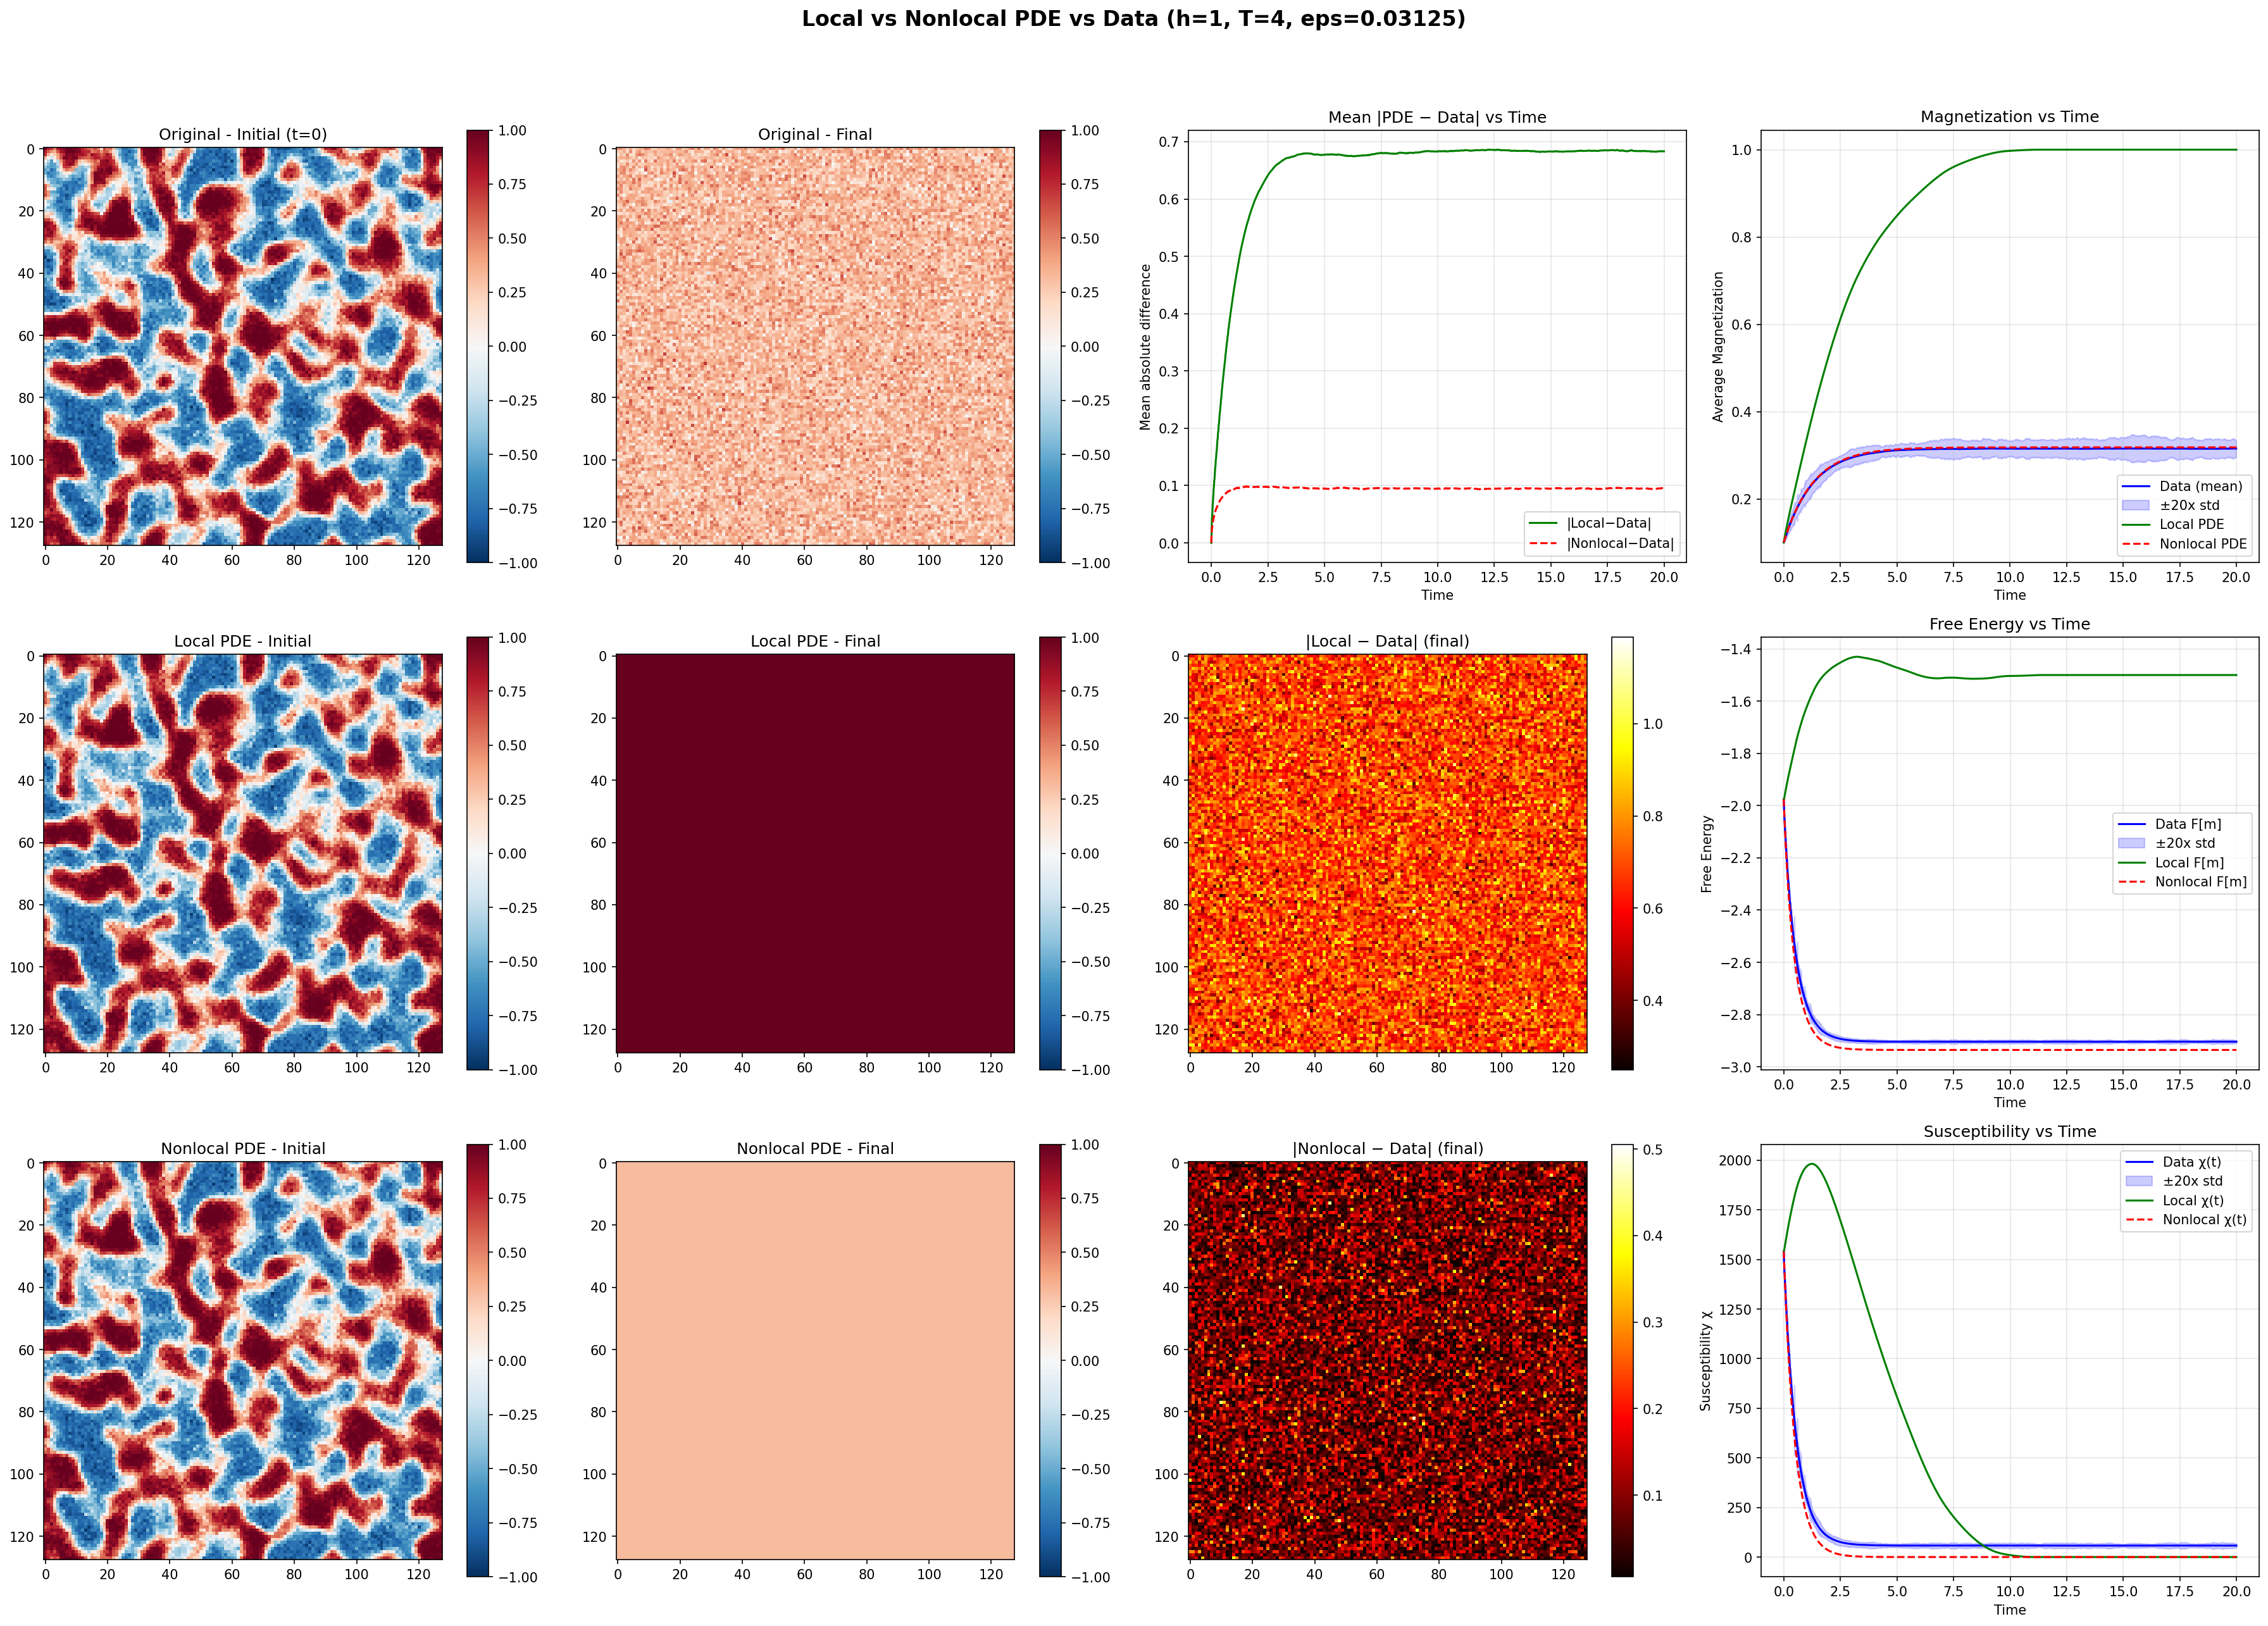
\includegraphics[width=1.0\textwidth]{fig/compare_local_nonlocal_L1024_h1_T4_eps0.03125.png}
    \caption{Comparison of original data and PDE solutions for $h=1$, $T=4$, $\epsilon=0.03125$, $L=1024$.}
    \label{fig:pde_comparison_h1_T4_eps0.03125}
\end{figure}



% with epsilon = 0.015625, L = 2048

\begin{figure}[!h]
    \centering
    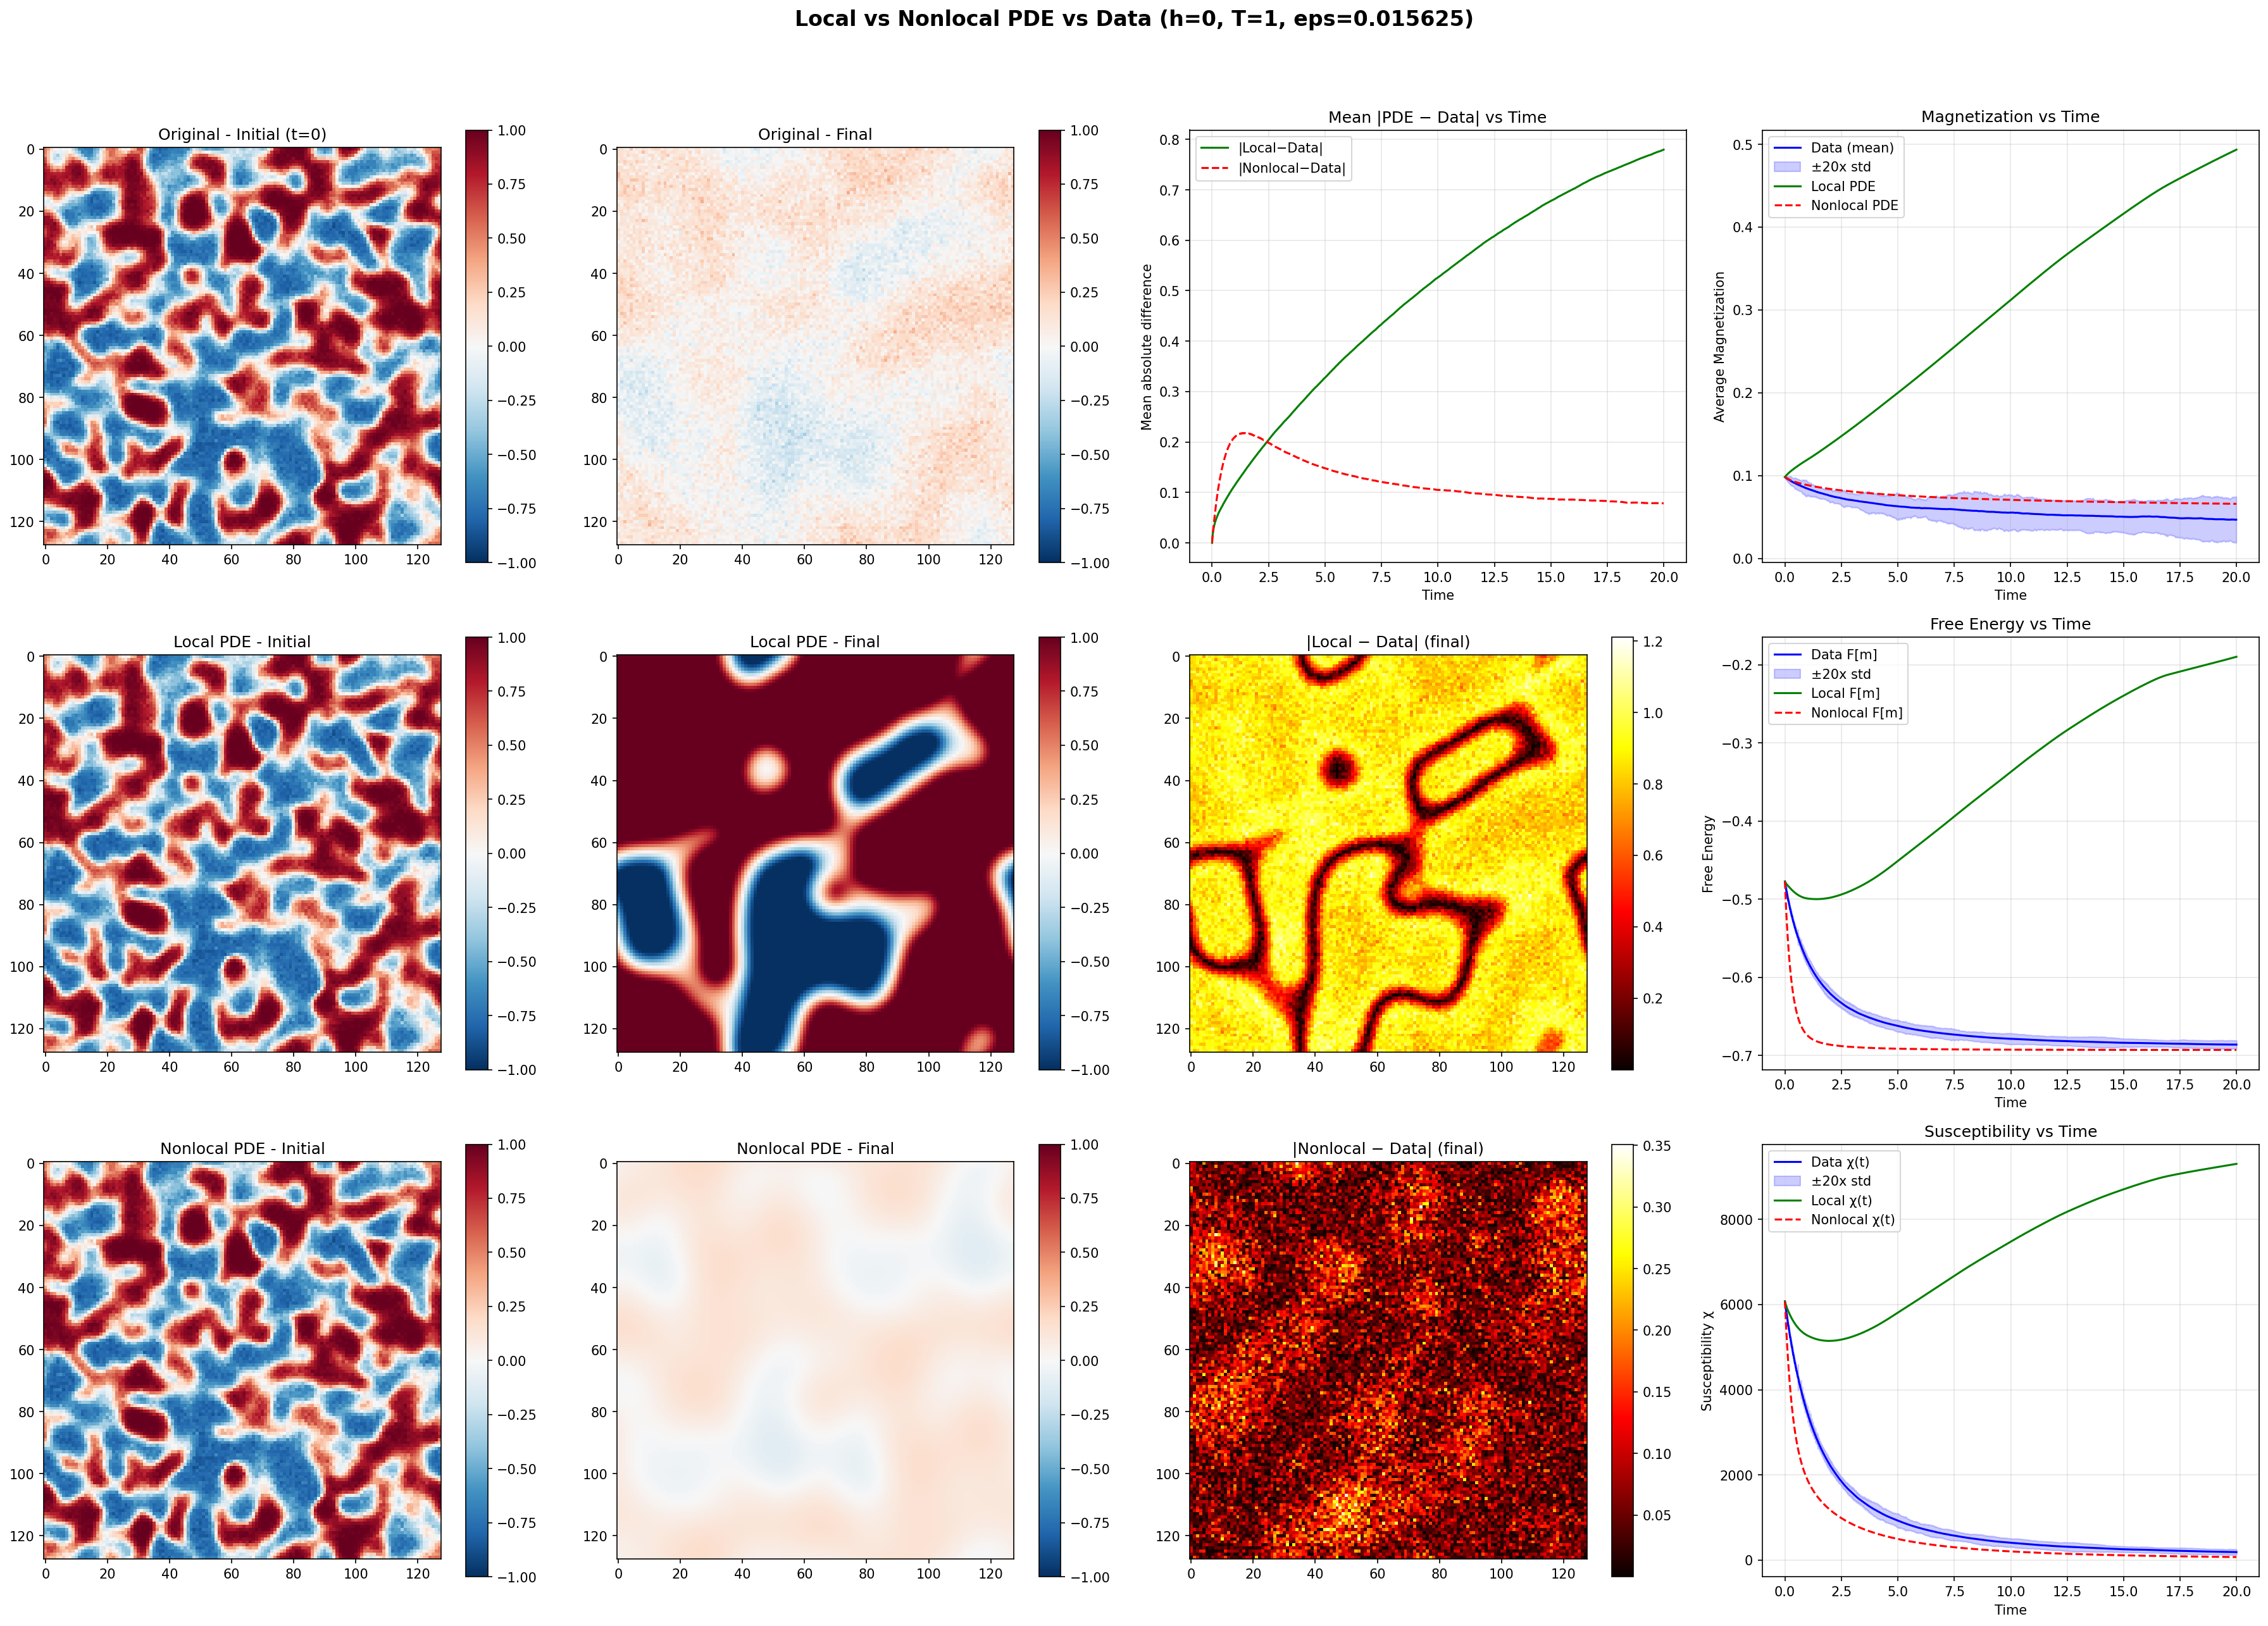
\includegraphics[width=1.0\textwidth]{fig/compare_local_nonlocal_L2048_h0_T1_eps0.015625.png}
    \caption{Comparison of original data and PDE solutions for $h=0$, $T=1$, $\epsilon=0.015625$, $L=2048$.}
    \label{fig:pde_comparison_h0_T1_eps0.015625_L2048}
\end{figure}


\begin{figure}[!h]
    \centering
    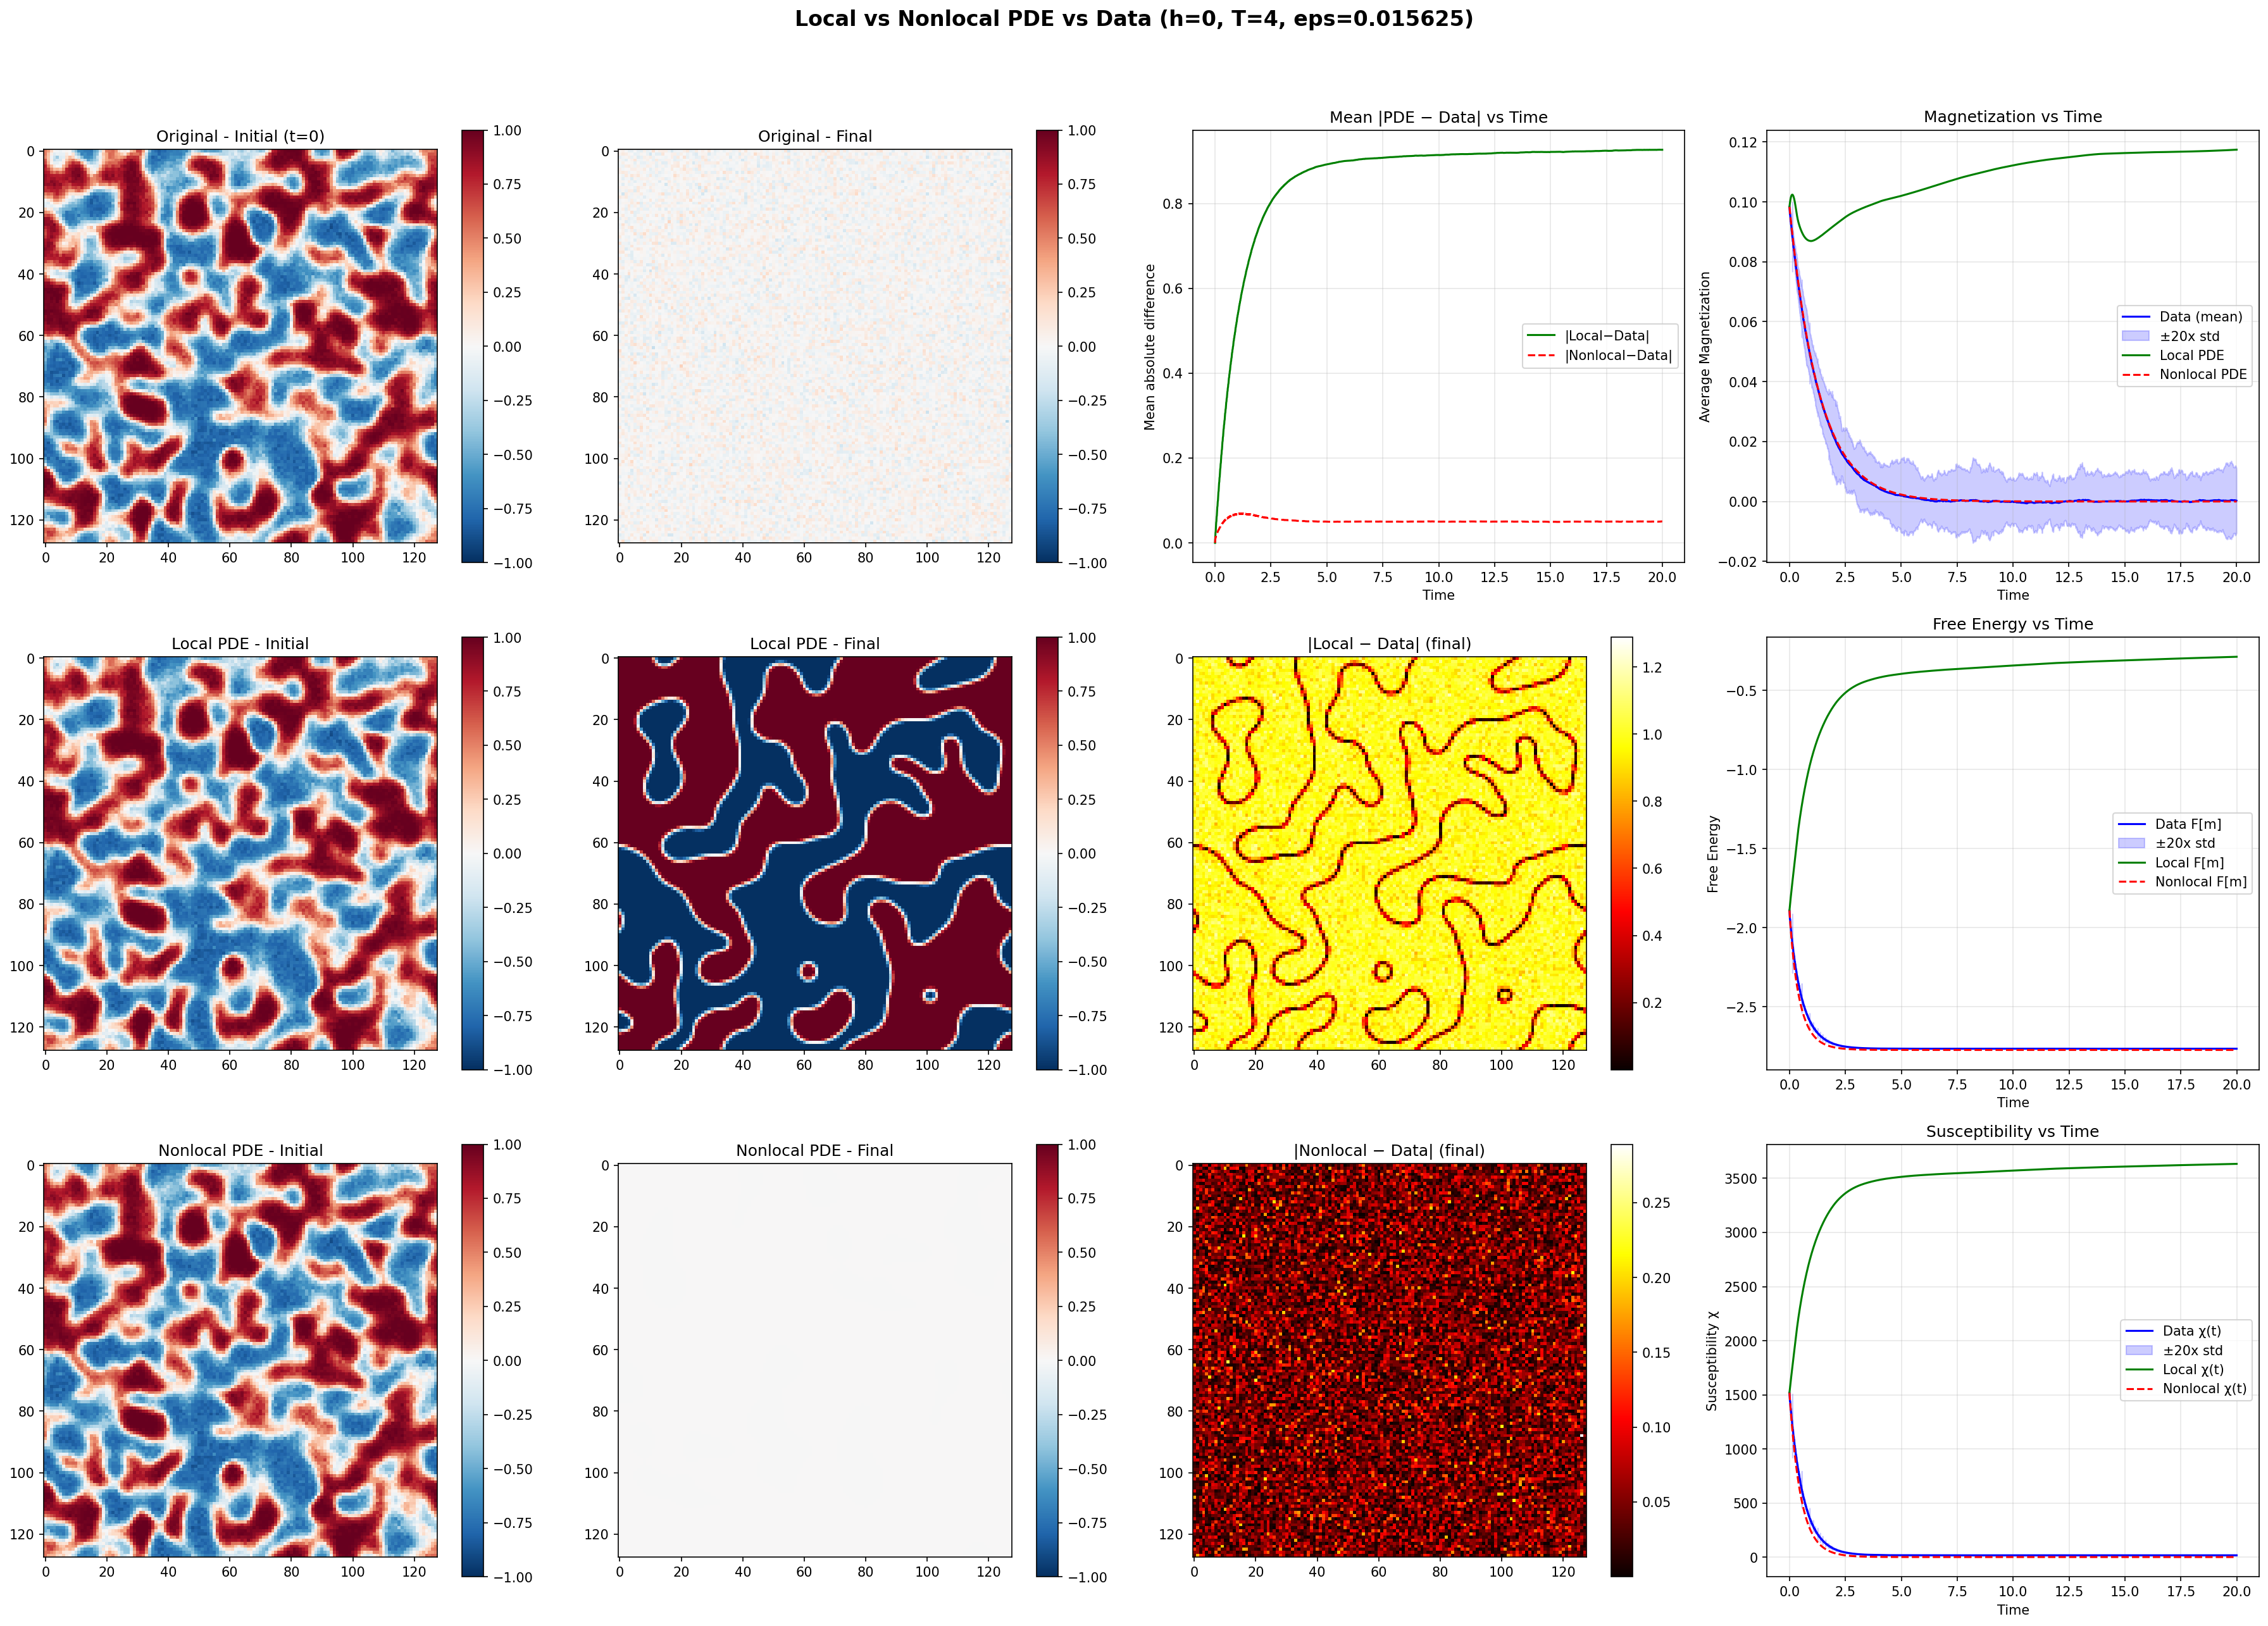
\includegraphics[width=1.0\textwidth]{fig/compare_local_nonlocal_L2048_h0_T4_eps0.015625.png}
    \caption{Comparison of original data and PDE solutions for $h=0$, $T=4$, $\epsilon=0.015625$, $L=2048$.}
    \label{fig:pde_comparison_h0_T4_eps0.015625_L2048}
\end{figure}


\begin{figure}[!h]
    \centering
    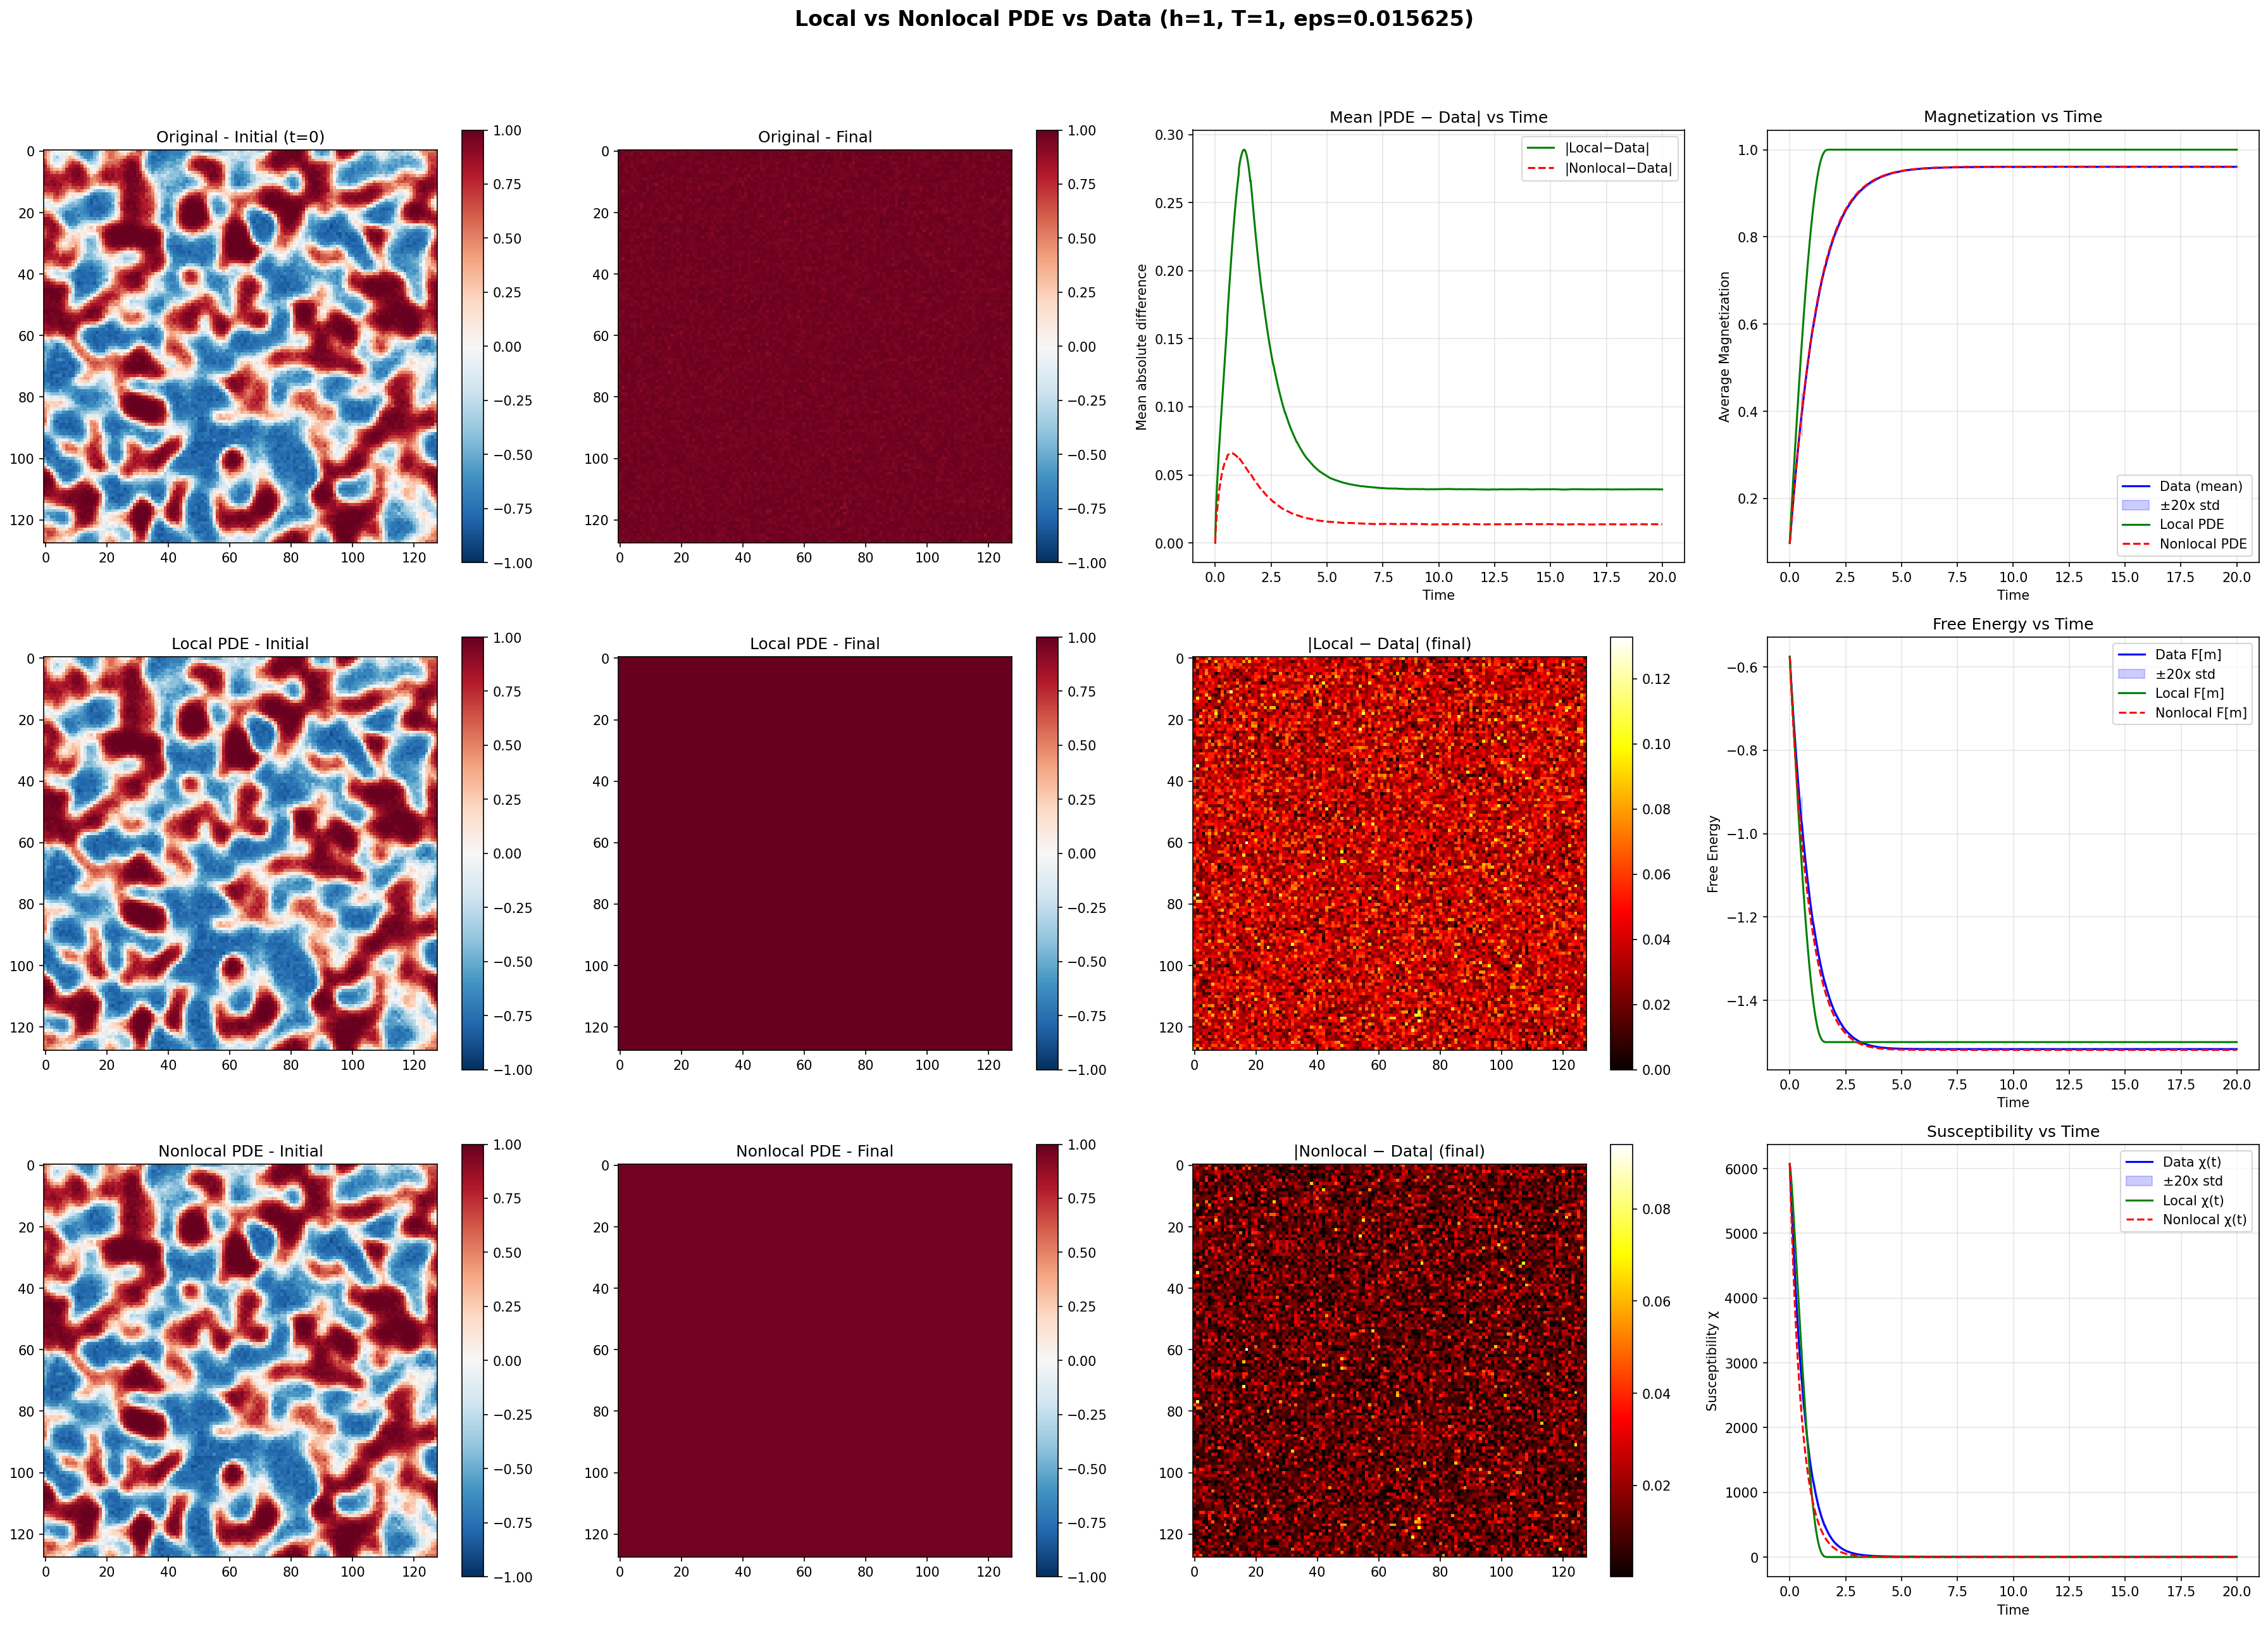
\includegraphics[width=1.0\textwidth]{fig/compare_local_nonlocal_L2048_h1_T1_eps0.015625.png}
    \caption{Comparison of original data and PDE solutions for $h=1$, $T=1$, $\epsilon=0.015625$, $L=2048$.}
    \label{fig:pde_comparison_h1_T1_eps0.015625_L2048}
\end{figure}


\begin{figure}[!h]
    \centering
    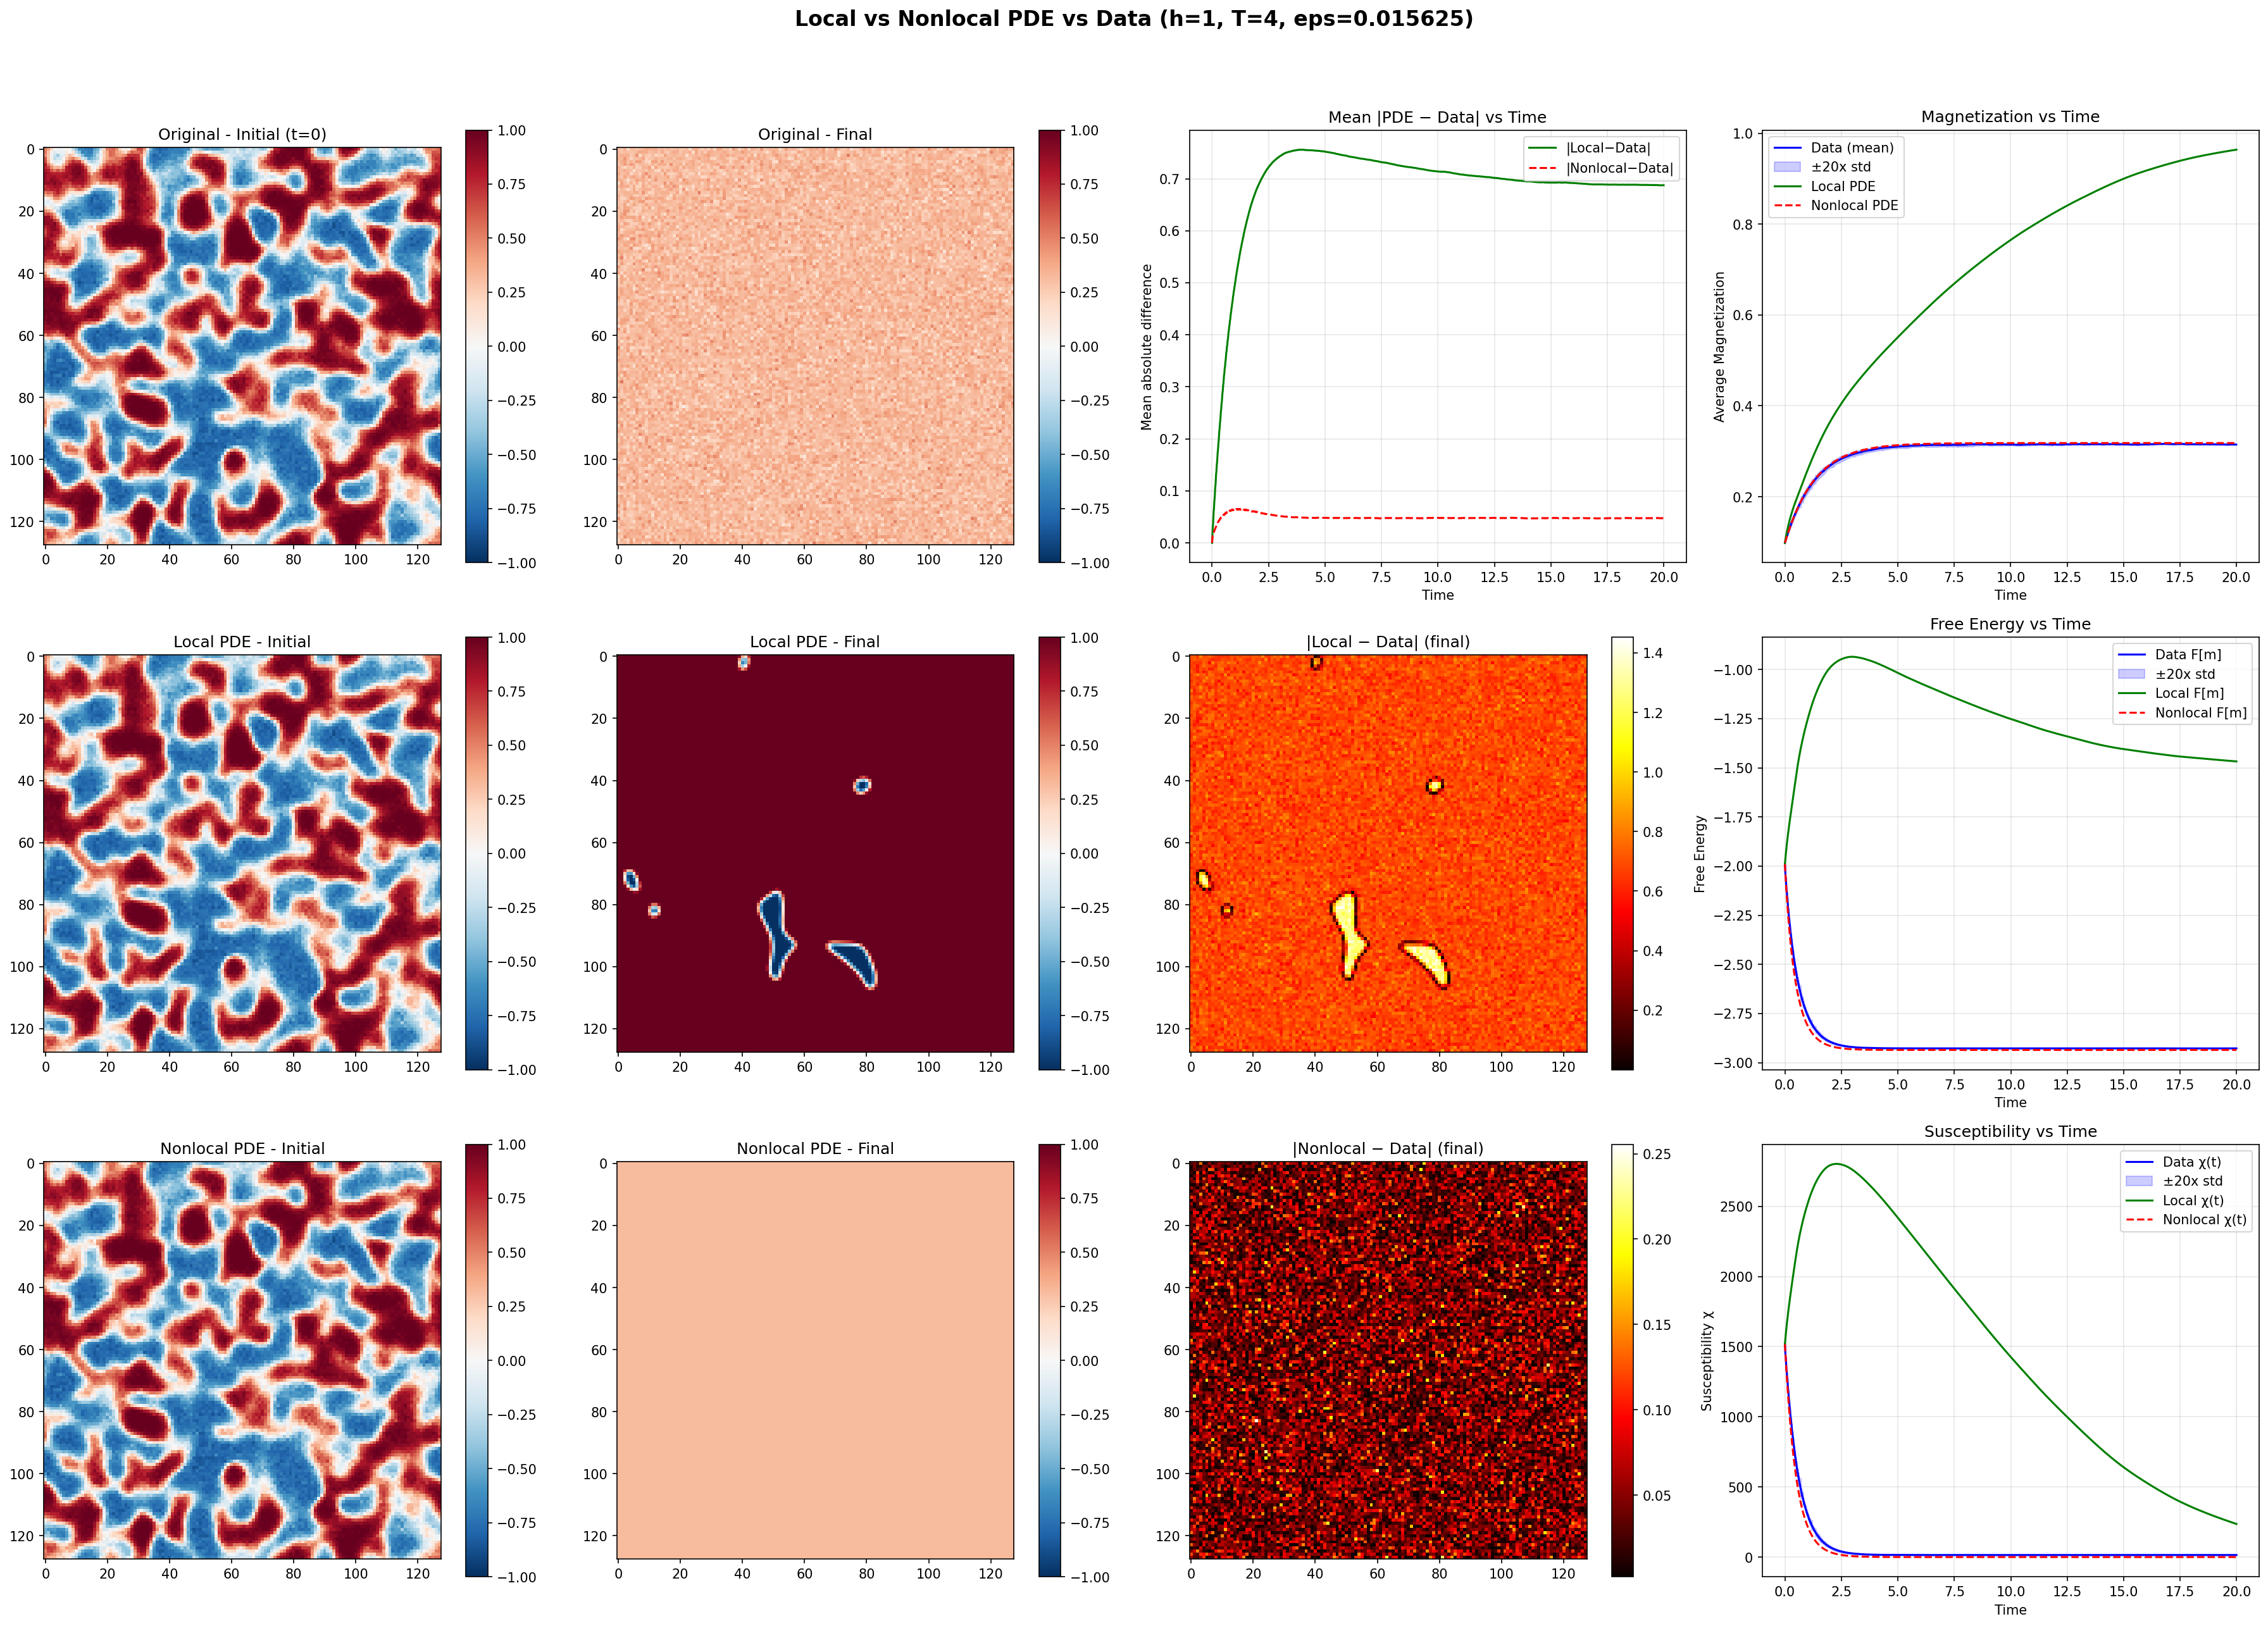
\includegraphics[width=1.0\textwidth]{fig/compare_local_nonlocal_L2048_h1_T4_eps0.015625.png}
    \caption{Comparison of original data and PDE solutions for $h=1$, $T=4$, $\epsilon=0.015625$, $L=2048$.}
    \label{fig:pde_comparison_h1_T4_eps0.015625_L2048}
\end{figure}

% with epsilon = 0.03125

\begin{figure}[!h]
    \centering
    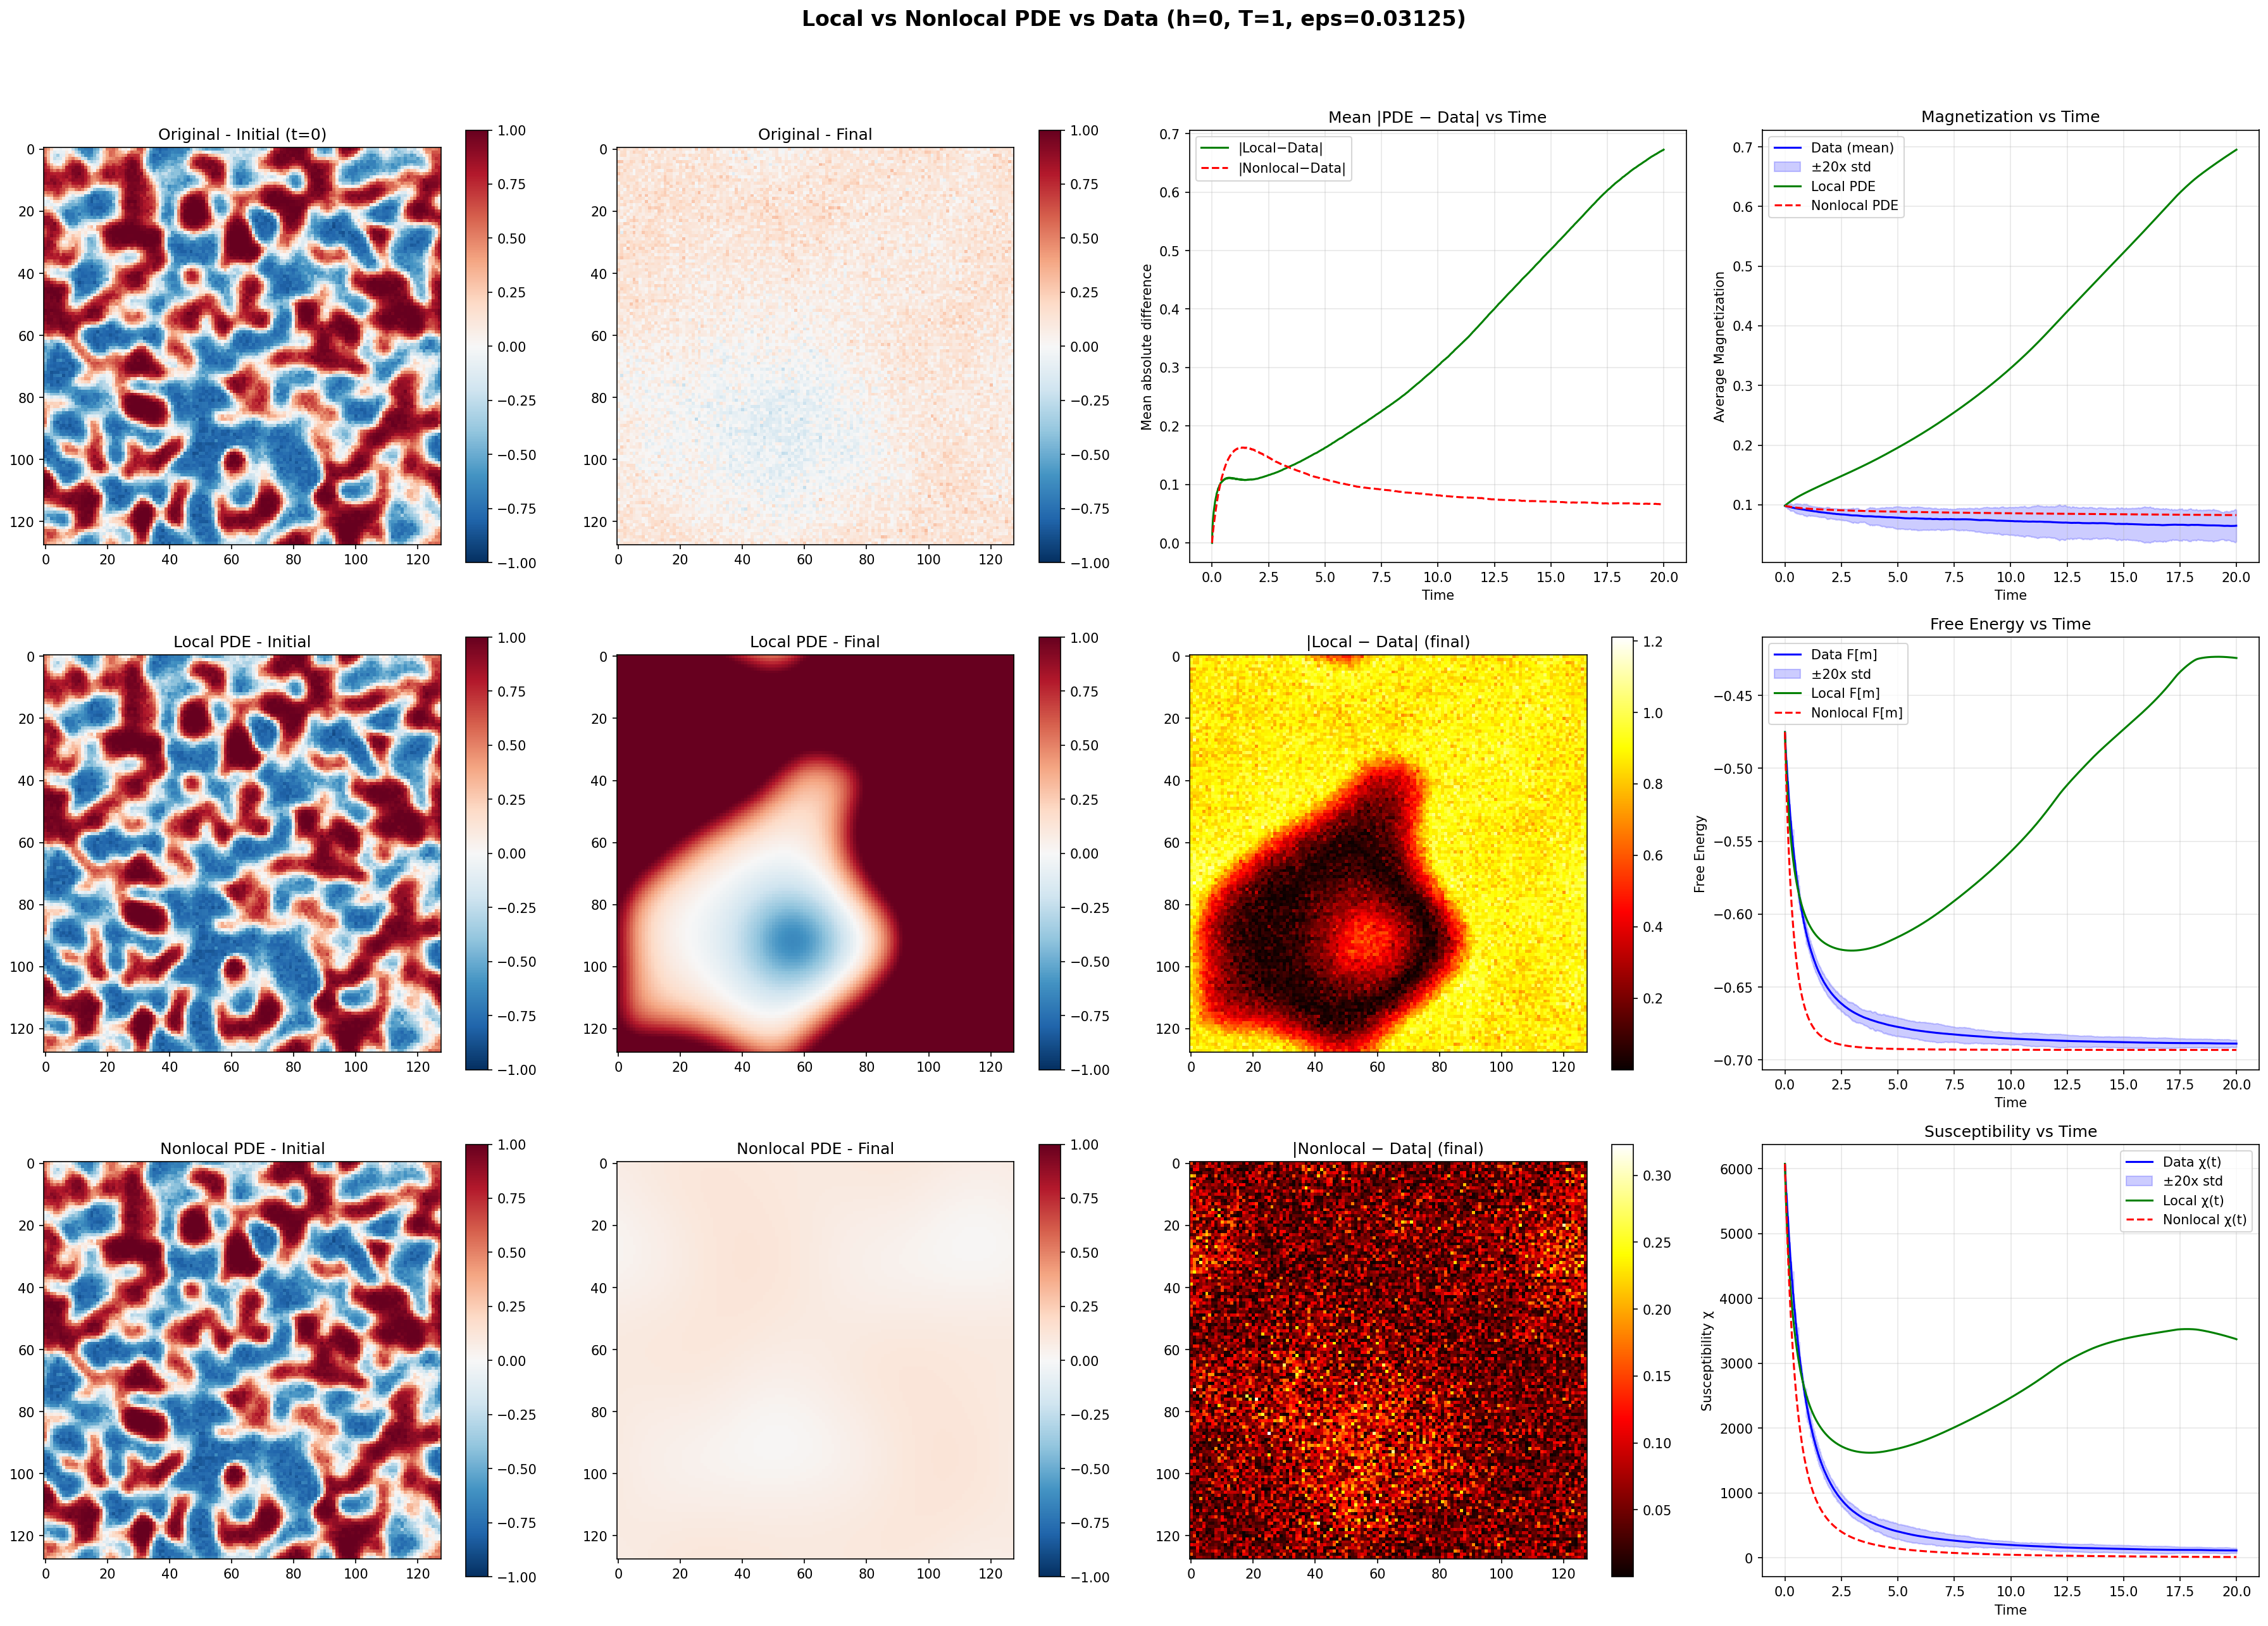
\includegraphics[width=1.0\textwidth]{fig/compare_local_nonlocal_L2048_h0_T1_eps0.03125.png}
    \caption{Comparison of original data and PDE solutions for $h=0$, $T=1$, $\epsilon=0.03125$, $L=2048$.}
    \label{fig:pde_comparison_h0_T1_eps0.03125_L2048}
\end{figure}


\begin{figure}[h]
    \centering
    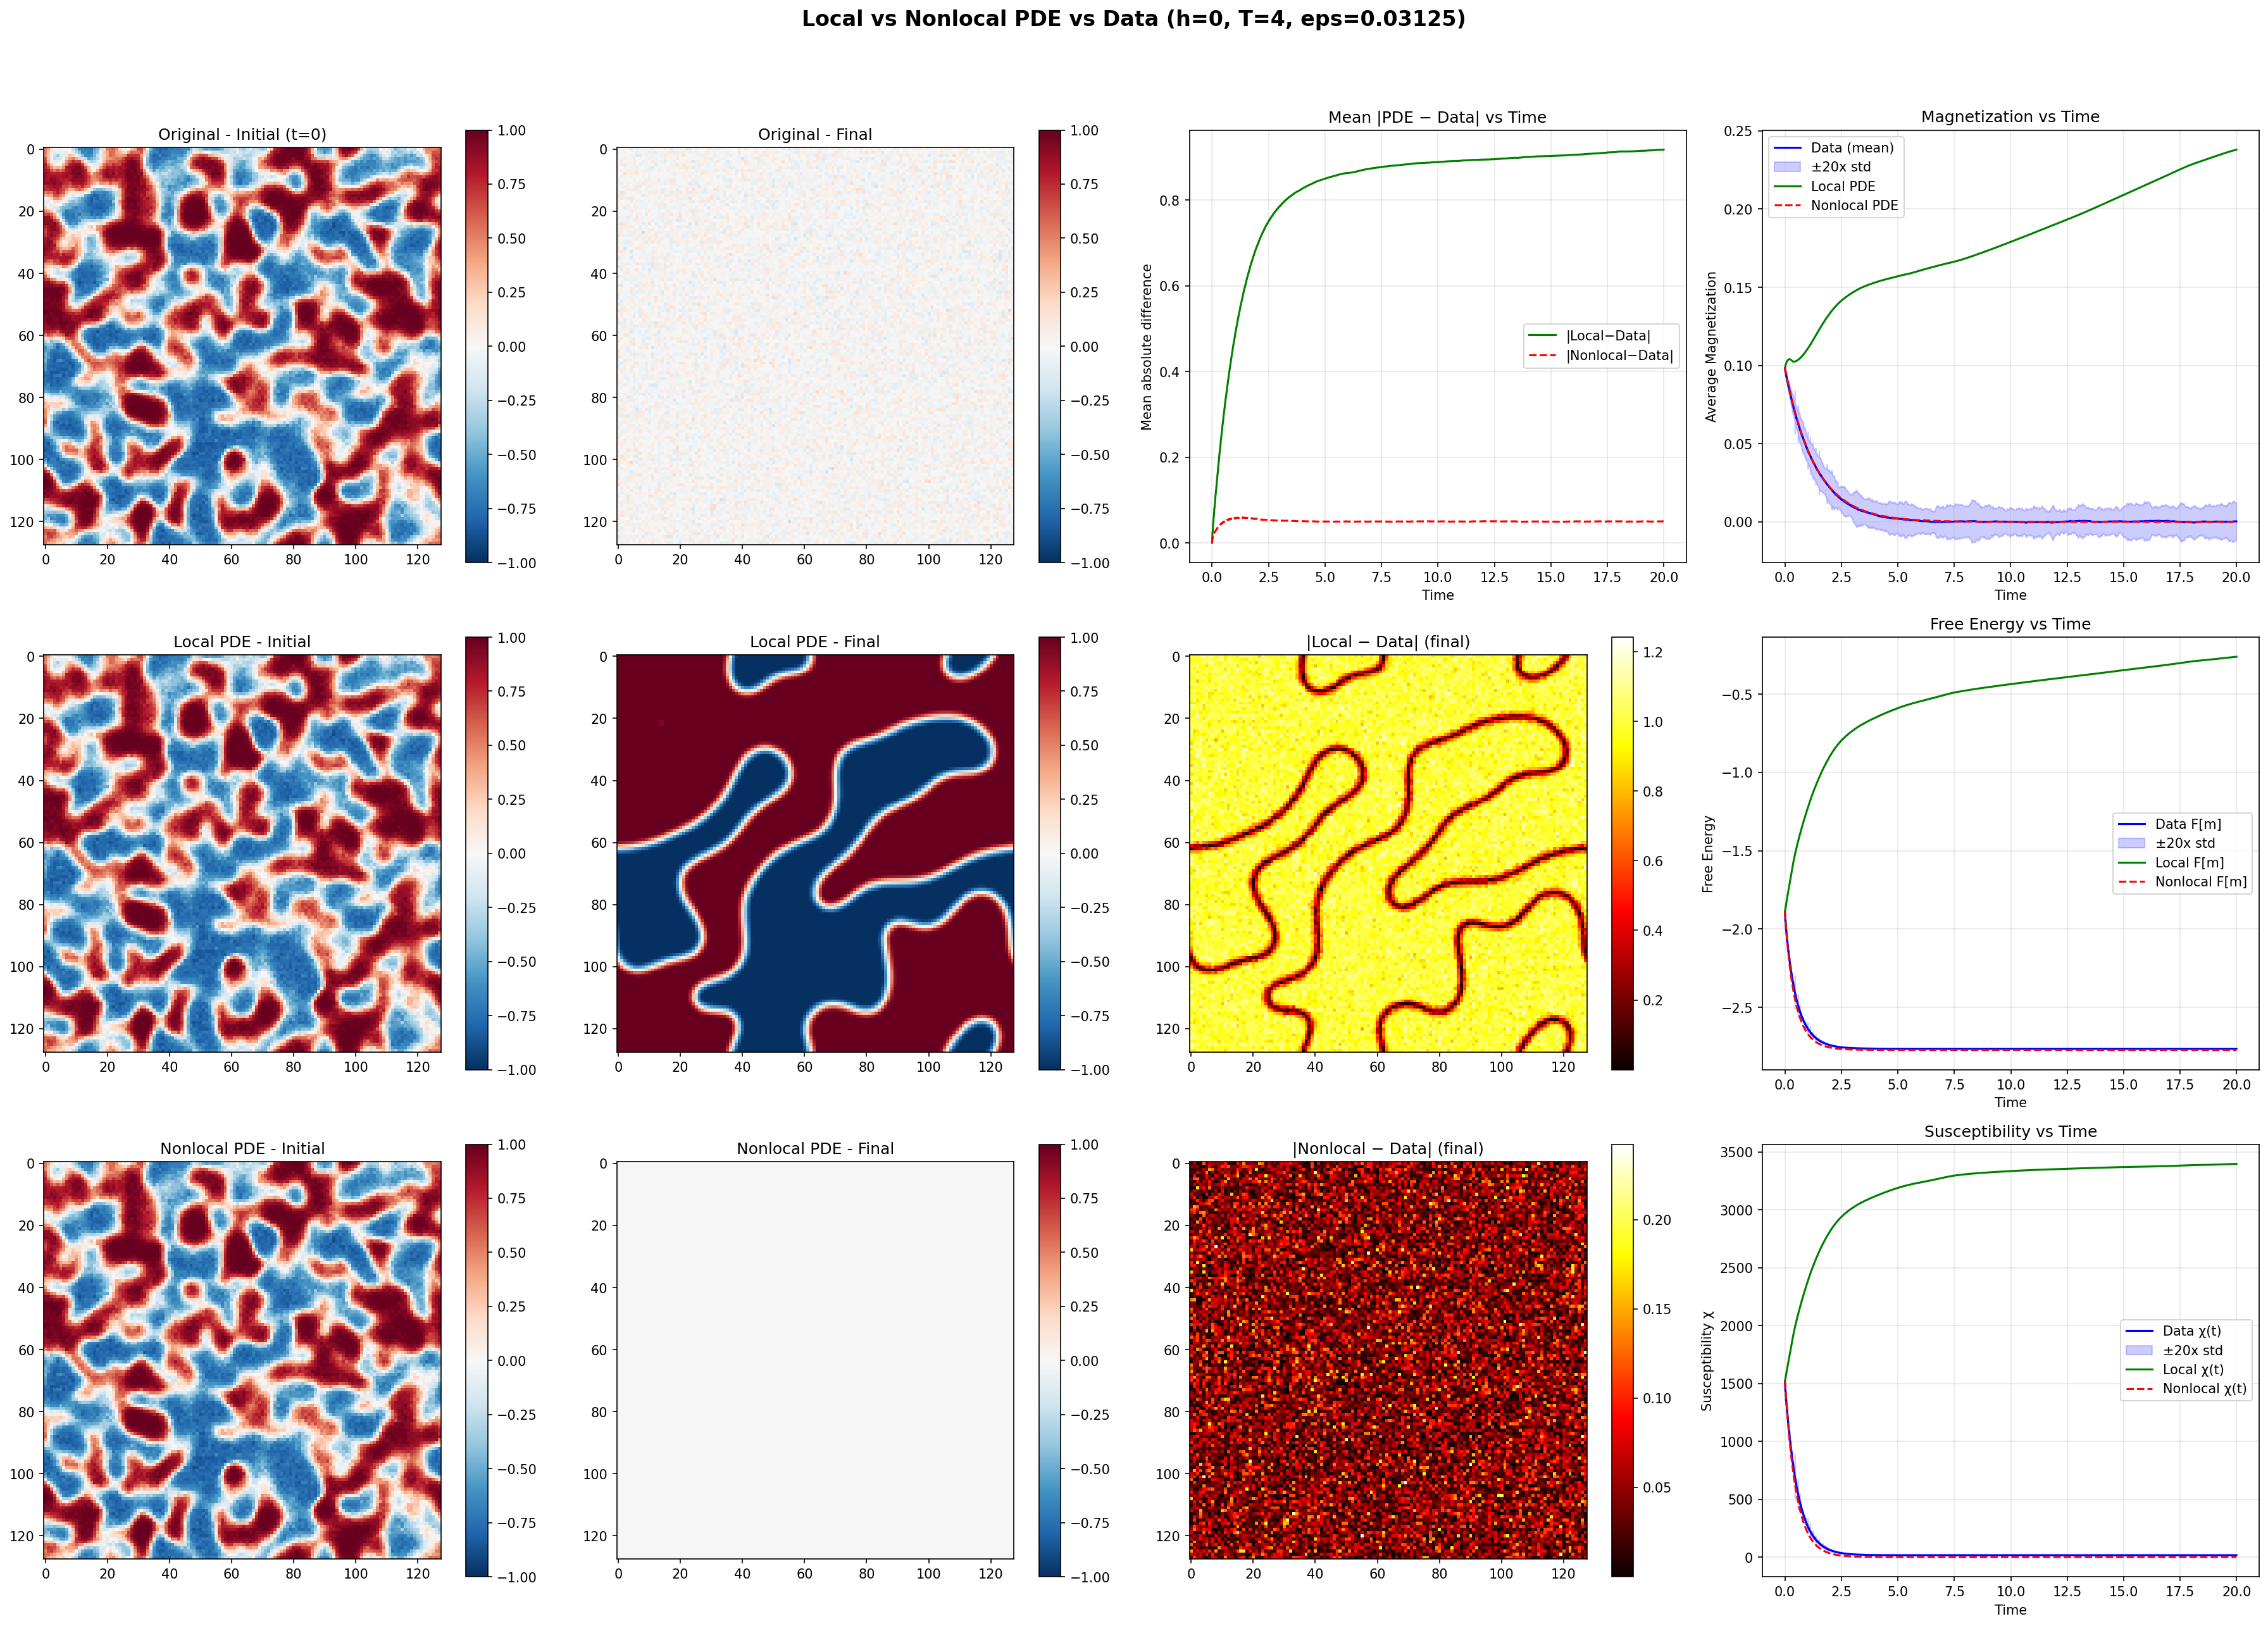
\includegraphics[width=1.0\textwidth]{fig/compare_local_nonlocal_L2048_h0_T4_eps0.03125.png}
    \caption{Comparison of original data and PDE solutions for $h=0$, $T=4$, $\epsilon=0.03125$, $L=2048$.}
    \label{fig:pde_comparison_h0_T4_eps0.03125_L2048}
\end{figure}


\begin{figure}[!h]
    \centering
    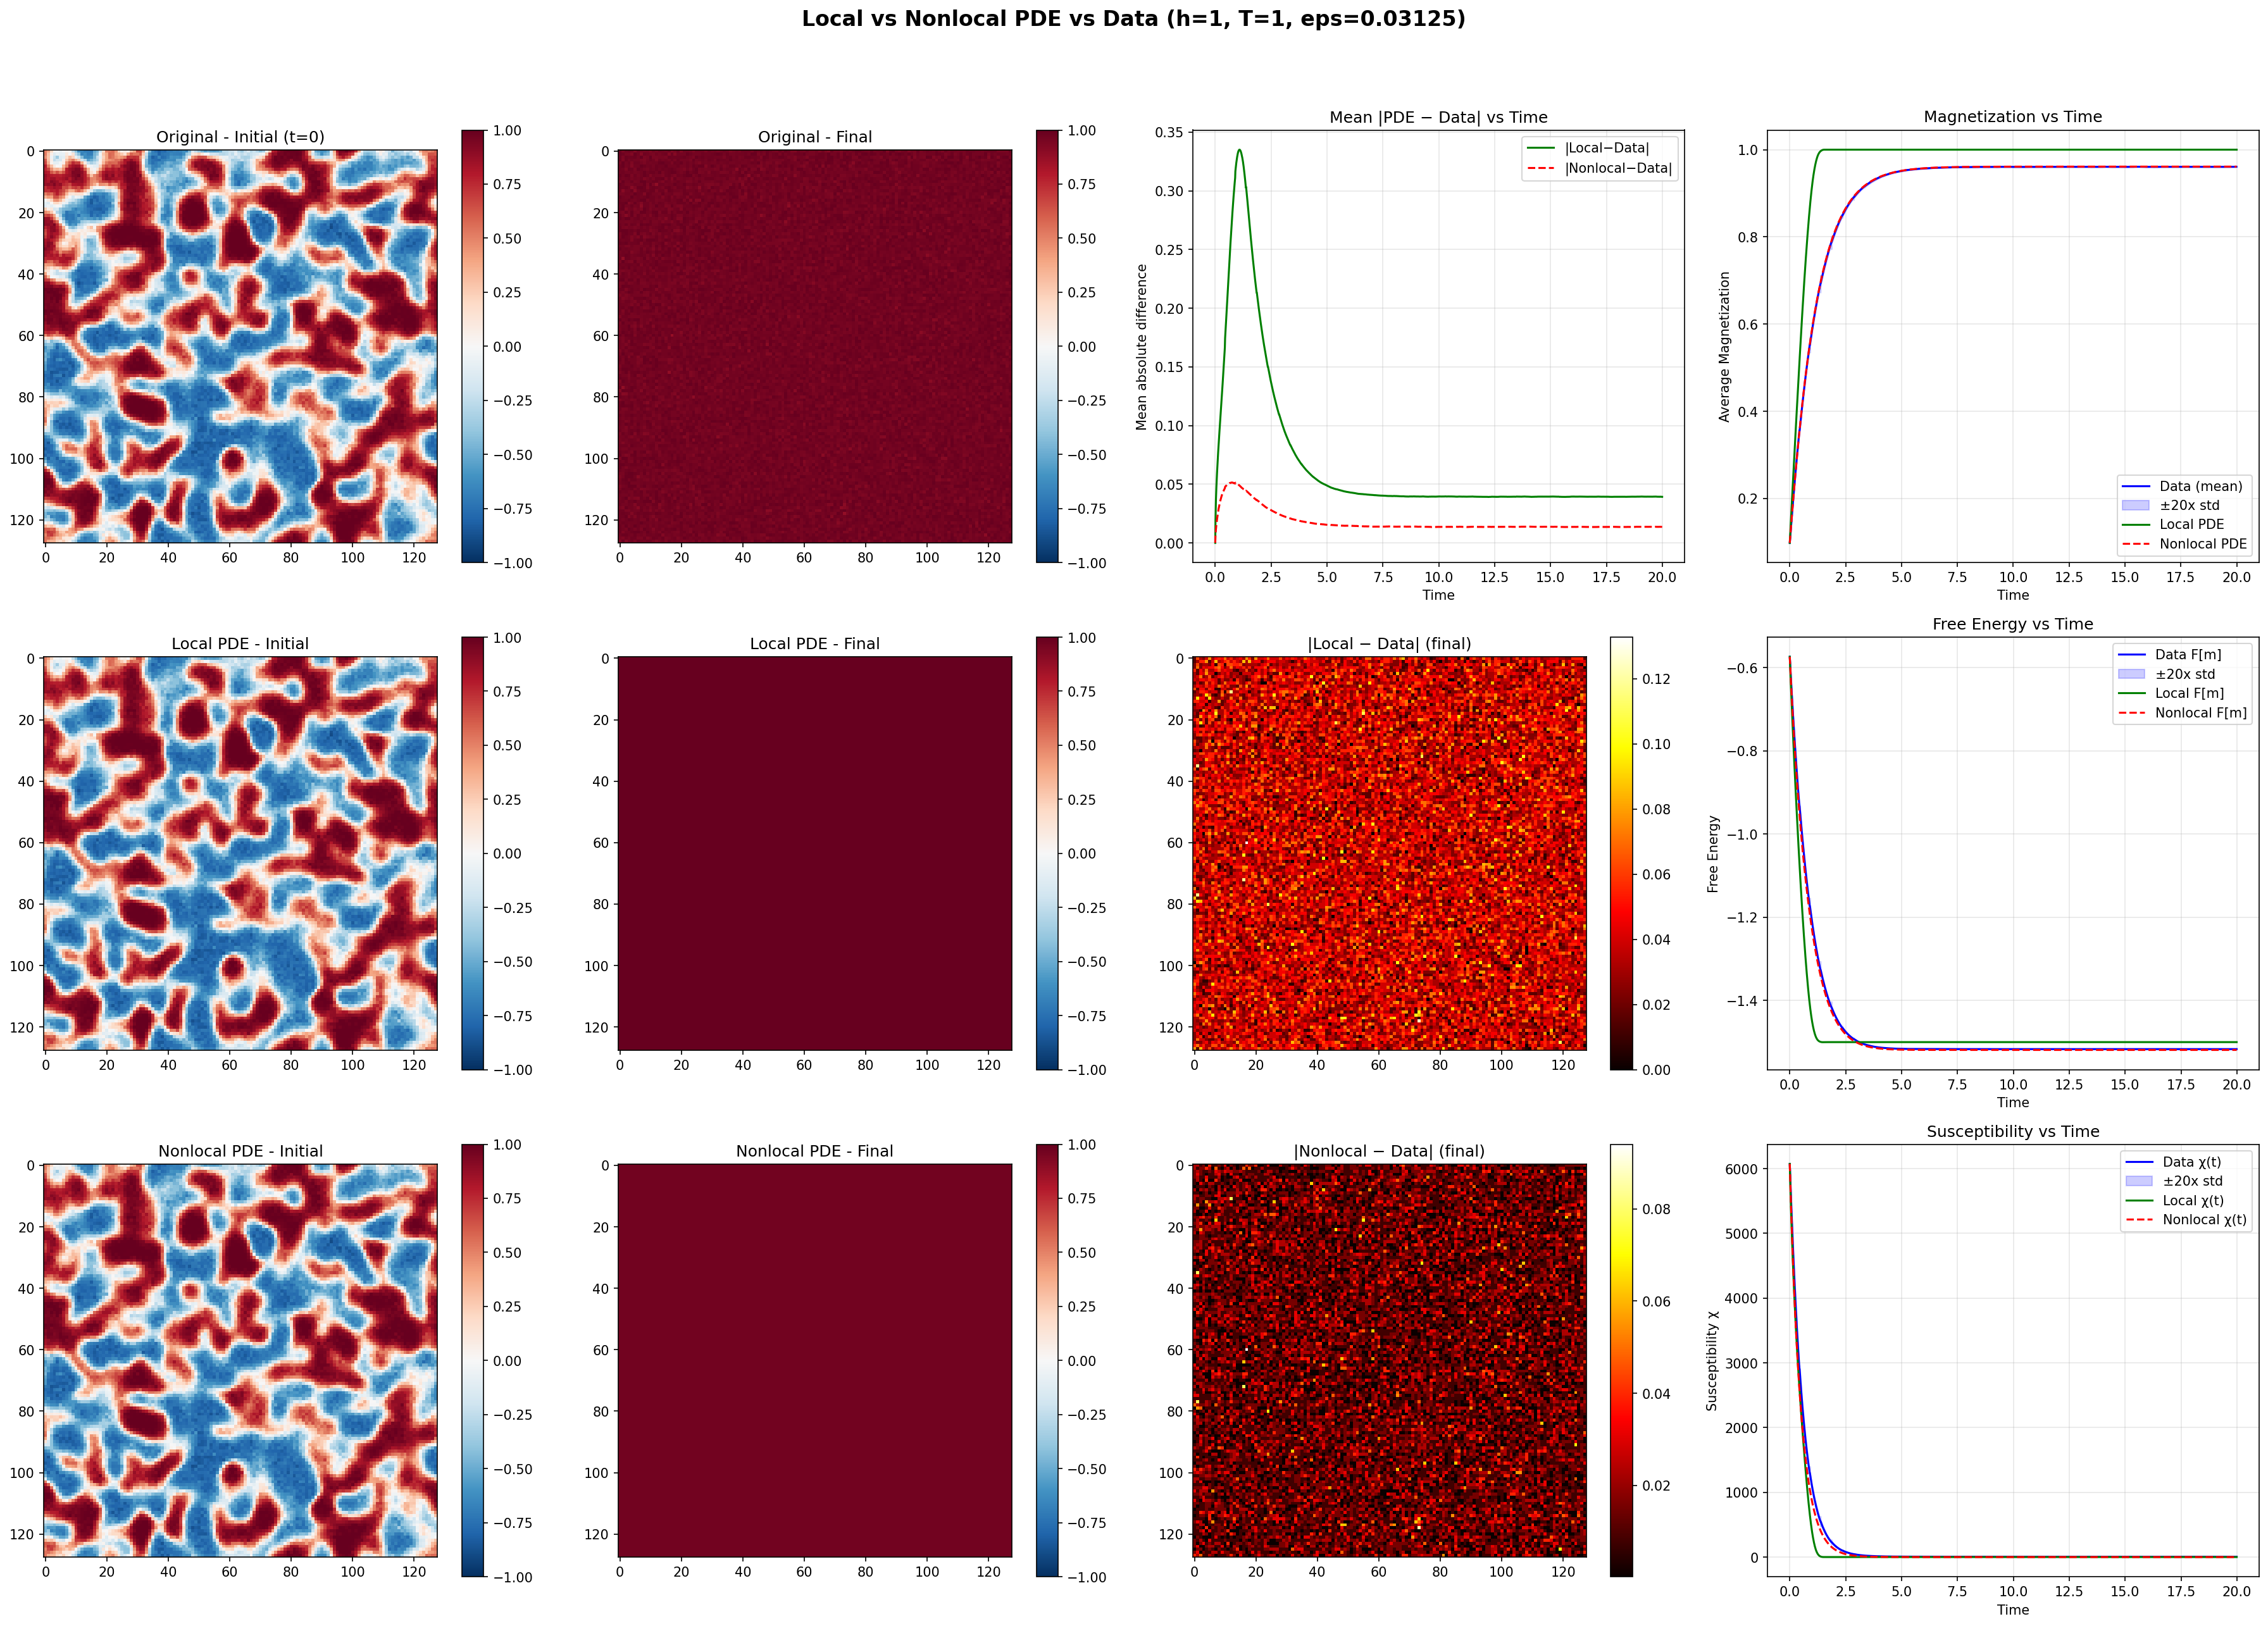
\includegraphics[width=1.0\textwidth]{fig/compare_local_nonlocal_L2048_h1_T1_eps0.03125.png}
    \caption{Comparison of original data and PDE solutions for $h=1$, $T=1$, $\epsilon=0.03125$, $L=2048$.}
    \label{fig:pde_comparison_h1_T1_eps0.03125_L2048}
\end{figure}


\begin{figure}[h]
    \centering
    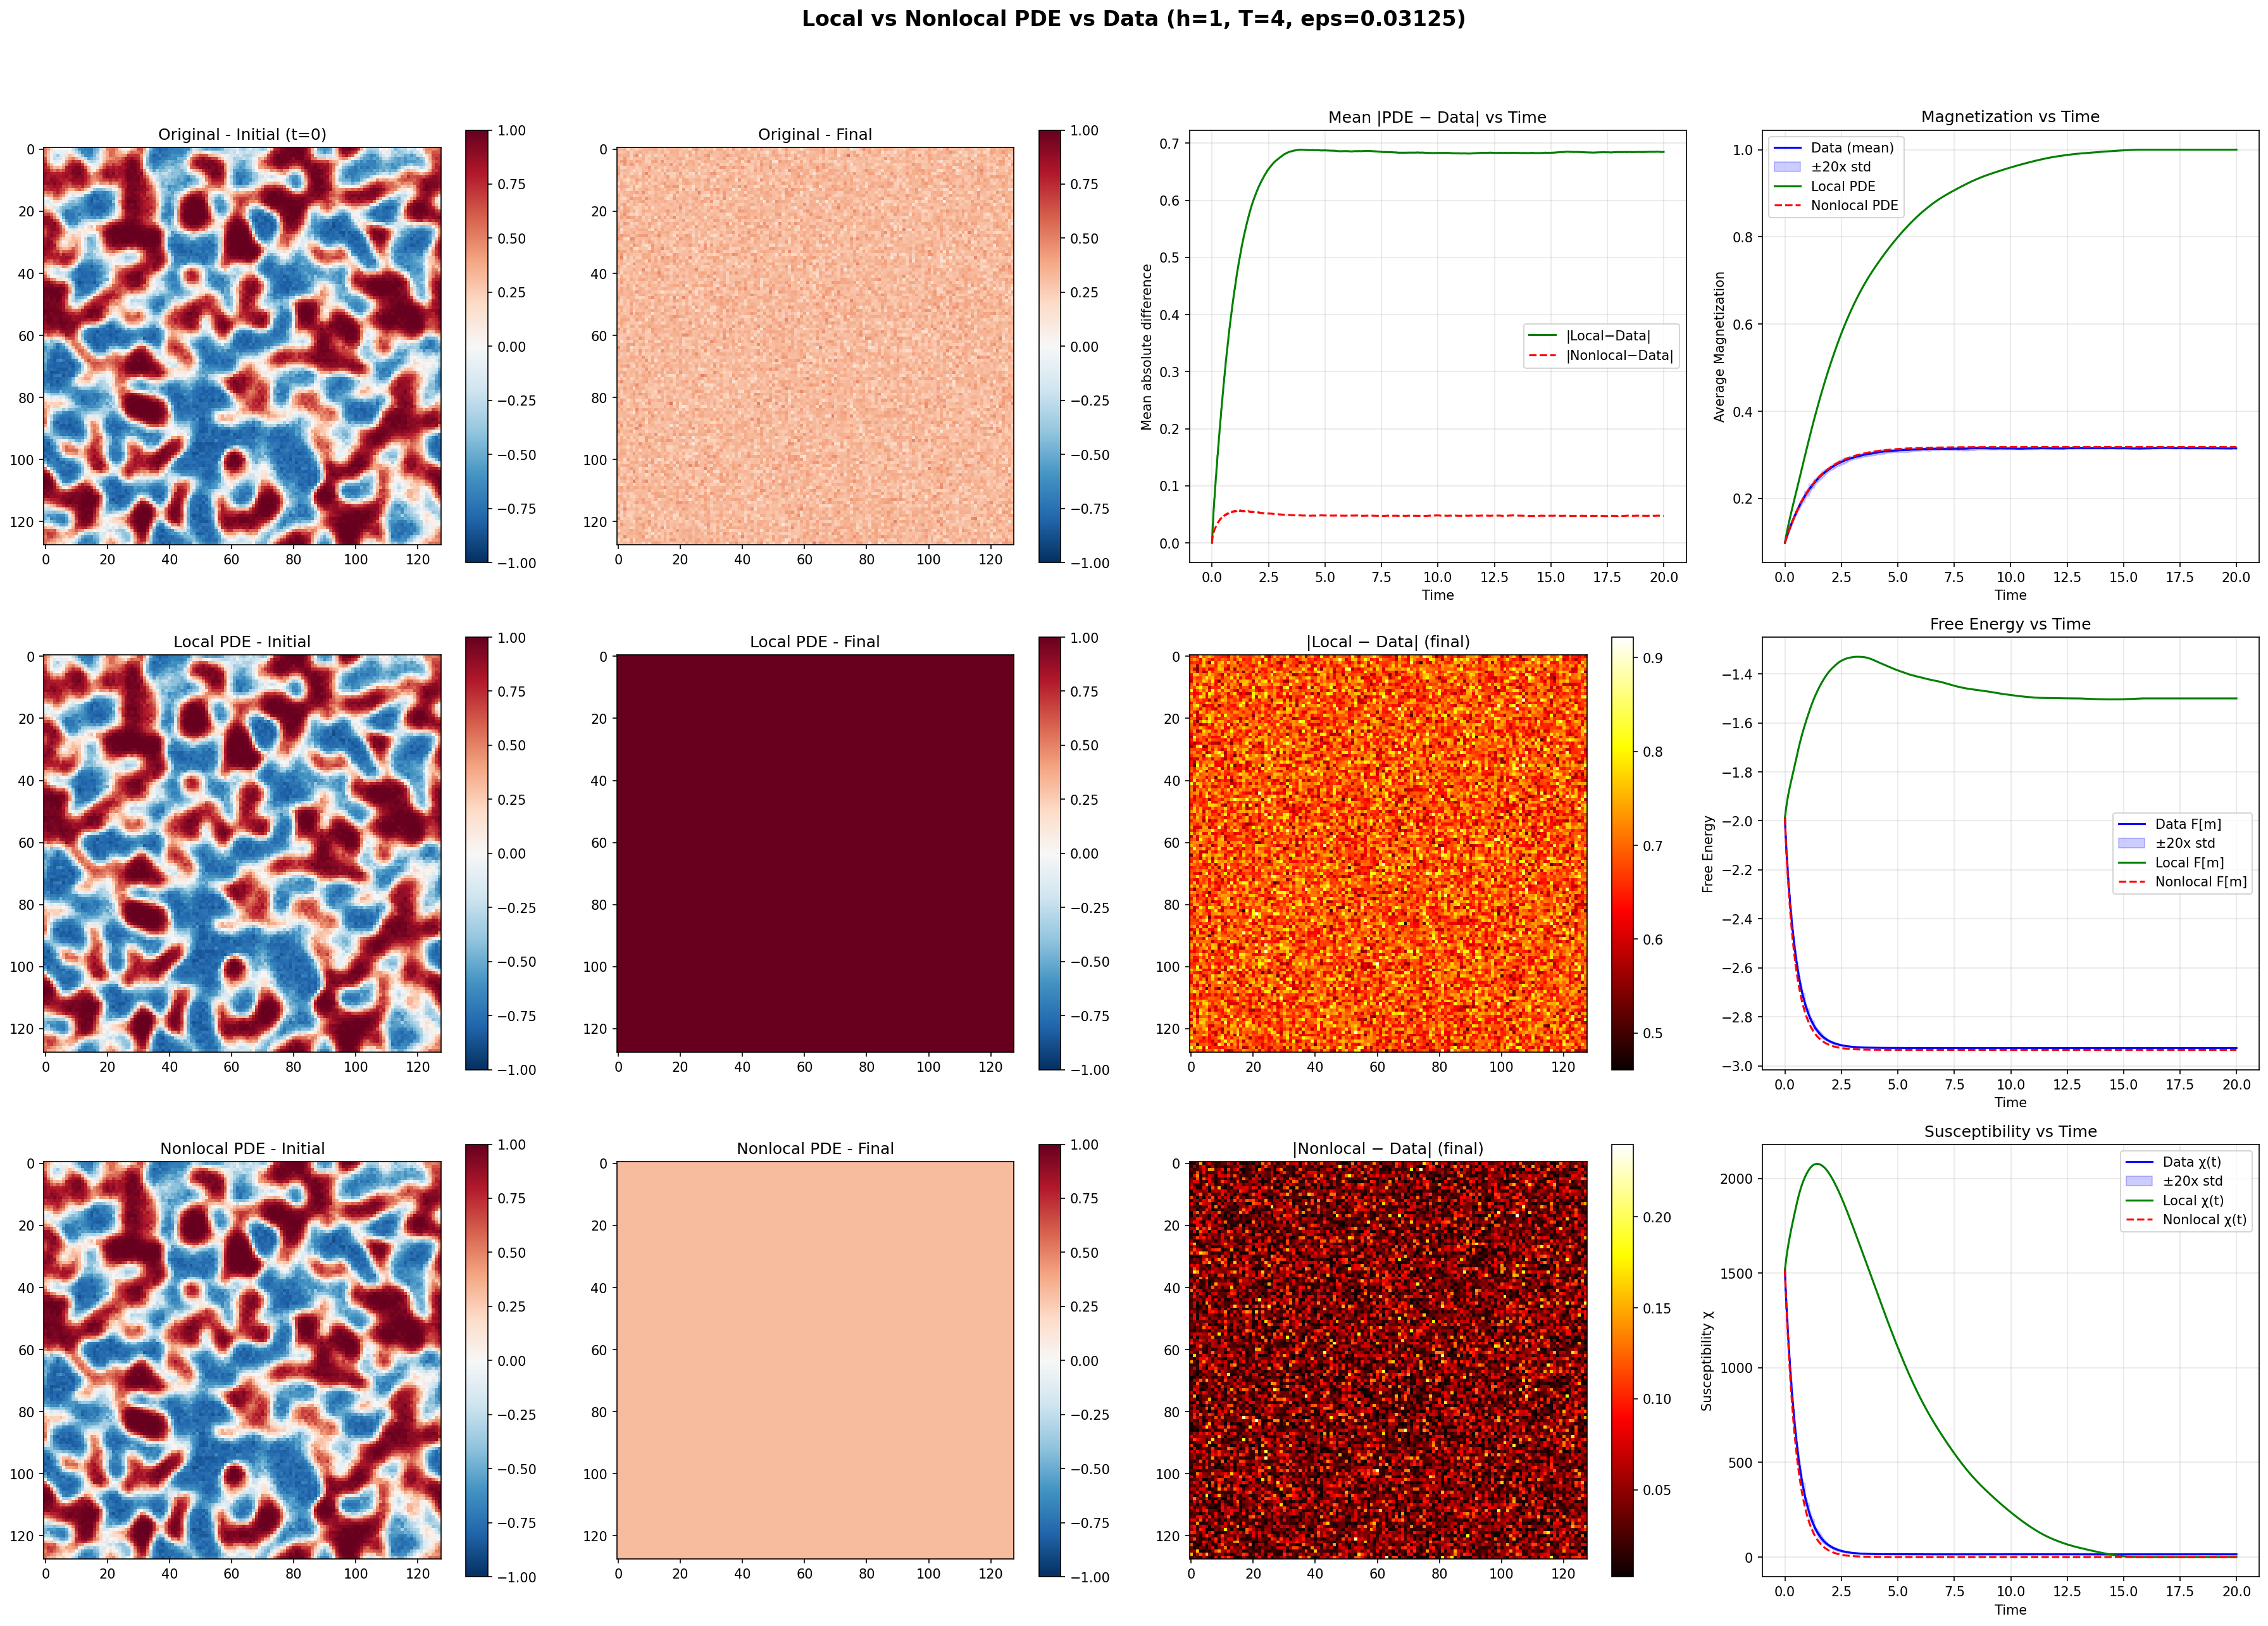
\includegraphics[width=1.0\textwidth]{fig/compare_local_nonlocal_L2048_h1_T4_eps0.03125.png}
    \caption{Comparison of original data and PDE solutions for $h=1$, $T=4$, $\epsilon=0.03125$, $L=2048$.}
    \label{fig:pde_comparison_h1_T4_eps0.03125_L2048}
\end{figure}



% ------------------------------------------------------------
\subsection{Error metric and statistical indicators used in comparisons}
\label{sec:error_and_stats}

We summarize the precise definitions of the error curves and the three statistical indicators displayed in the comparison figures (data, local PDE, nonlocal PDE). We work on the periodic domain $\Omega=[0,1]^2$ discretized by an $M\times M$ grid with spacing $\Delta x = \Delta y = 1/M$ and $N=M^2$ grid points. Spatial integrals are approximated by Riemann sums with weight $\Delta x\,\Delta y = 1/M^2$.

\paragraph{Time alignment.} Let $\{t^{\text{data}}_n\}_{n=0}^{T_{\text{data}}-1}$, $\{t^{\text{loc}}_n\}_{n=0}^{T_{\text{loc}}-1}$ and $\{t^{\text{non}}_n\}_{n=0}^{T_{\text{non}}-1}$ denote the sampled times for the data, local PDE, and nonlocal PDE trajectories, respectively. For plotting time series jointly, we form a common index set of length $T_\ast=\min(T_{\text{data}},T_{\text{loc}},T_{\text{non}})$ by taking linearly spaced integer indices into each sequence (nearest-neighbor subsampling). We denote the aligned fields by $m_{\text{data}}(t_i,\cdot)$, $m_{\text{loc}}(t_i,\cdot)$, and $m_{\text{non}}(t_i,\cdot)$ for $i=0,\dots,T_\ast-1$.

\paragraph{Magnetization (spatial mean).} For any field $m(t,\cdot)$,
\begin{equation}
    \overline{m}(t) \;=\; \frac{1}{|\Omega|} \int_{\Omega} m(t,\mathbf{x})\,d\mathbf{x}
    \;\approx\; \frac{1}{M^2} \sum_{i,j=0}^{M-1} m_{i,j}(t).
\end{equation}
We plot $\overline{m}_{\text{data}}(t_i)$, $\overline{m}_{\text{loc}}(t_i)$, and $\overline{m}_{\text{non}}(t_i)$ on a shared time axis.

\paragraph{Free energy used in plots (post-processing functional).} Let $\beta>0$ be the inverse temperature, $h\in\mathbb{R}$ the external field, $J_0\in\mathbb{R}$ an interaction-strength factor, and $J$ a nonnegative, radially symmetric, \emph{sum-normalized} kernel (i.e., the discrete sum of $J$ over the periodic grid equals one). Define $p=(1+m)/2$ and $q=(1-m)/2$. The free energy density used in the plots is
\begin{equation}
    f(m) \;=\; \frac{1}{\beta}\Big( p\,\ln p + q\,\ln q \Big)
    \; -\; \frac{J_0}{2}\, m\, (J*m)
    \; -\; h\, m,
\end{equation}
and the post-processed free energy is
\begin{equation}
    F[m](t) \;=\; \int_{\Omega} f\big(m(t,\mathbf{x})\big)\,d\mathbf{x}
    \;\approx\; \frac{1}{M^2} \sum_{i,j=0}^{M-1} \Bigg[ \frac{1}{\beta}\Big( p_{i,j}\ln p_{i,j} + q_{i,j}\ln q_{i,j} \Big)
    - \frac{J_0}{2}\, m_{i,j}\, (J*m)_{i,j}
    - h\, m_{i,j} \Bigg].
\end{equation}
Here $(J*m)$ is the \emph{periodic} convolution of $m$ with $J$ on the $M\times M$ grid; in computations it is obtained by constructing $J$ in real space, normalizing to unit discrete sum, applying $\mathrm{ifftshift}$, taking its $\mathrm{fft2}$, and multiplying in Fourier space before an inverse FFT.

\emph{Remark.} This plotted functional differs from the theoretical Lyapunov functional in \cref{sec:nonlocal_theory} by constant shifts and scaling conventions (e.g., factors of $\beta$ and $J_0$); it is chosen to match the numerical post-processing used across data/local/nonlocal trajectories.

\paragraph{Magnetic susceptibility.} The spatial susceptibility is computed as
\begin{equation}
    \chi(t) \;=\; \beta\,N\,\Big( \langle m^2(t,\cdot)\rangle_x - \langle m(t,\cdot)\rangle_x^{\,2} \Big),
\end{equation}
where $\langle\cdot\rangle_x$ denotes the spatial average over the grid, i.e., $\langle m\rangle_x = M^{-2}\sum m_{i,j}$ and $N=M^2$. We plot $\chi_{\text{data}}(t_i)$, $\chi_{\text{loc}}(t_i)$, and $\chi_{\text{non}}(t_i)$ on a shared time axis.

\paragraph{Mean absolute error curves.} The error curves shown are the \emph{spatial mean absolute error} between PDE solutions and data at aligned times:
\begin{equation}
    E_{\text{loc}}(t_i) \;=\; \frac{1}{M^2} \sum_{k,\ell=0}^{M-1} \big|\, m_{\text{loc};\,k\ell}(t_i) - m_{\text{data};\,k\ell}(t_i) \,\big|,
    \qquad
    E_{\text{non}}(t_i) \;=\; \frac{1}{M^2} \sum_{k,\ell=0}^{M-1} \big|\, m_{\text{non};\,k\ell}(t_i) - m_{\text{data};\,k\ell}(t_i) \,\big|.
\end{equation}
These correspond to the $\textit{Mean $|\mathrm{PDE}-\mathrm{Data}|$ vs Time}$ panel.

\section{Network Training}

Recall that we want to train a network to predict the dynamics of the system.

\begin{equation}\label{eq:nonlocal-recall}
\partial_t m(t,x) \;=\; -\,m(t,x)\;+\;\tanh\!\Big(\beta\, (J_\gamma * m)(t,x) + \beta h\Big), \qquad m(0,x)=m_0(x),
\end{equation}

\section{Theoretical analysis of the nonlocal Glauber--Kac PDE (GPT-generated, to be checked)} 
\label{sec:nonlocal_theory}

We summarize key analytical properties of the nonlocal evolution \eqref{eq:nonlocal-recall} on the periodic domain $\Omega=\mathbb{T}^d$, where the Kac kernel $J_\gamma$ is nonnegative and normalized (so that $\int_\Omega J_\gamma = 1$), and $\beta>0$ and $h\in\mathbb{R}$ are fixed parameters.

\subsection{Well-posedness and invariant bounds}
Let $\mathcal{J}[m] = (J_\gamma * m)$ denote periodic convolution. The right-hand side
\[
\mathcal{F}[m] \;=\; -m + \tanh\big(\beta\,(\mathcal{J}[m] + h)\big)
\]
is locally Lipschitz on $L^\infty(\Omega)$ because $\tanh$ is globally Lipschitz and $\mathcal{J}$ is a bounded linear operator on $L^\infty$. Hence, for any $m_0\in L^\infty$, there exists a unique mild/strong solution $m(t)\in C([0,\infty);L^\infty)$.

Moreover, the interval $(-1,1)$ is invariant: if $\|m_0\|_{L^\infty}\le 1$, then $\|m(t)\|_{L^\infty}<1$ for all $t>0$. Indeed, for any fixed $x$, the map $u\mapsto -u+\tanh(\beta a)$ with $a\in\mathbb{R}$ points inward at $u=\pm1$ since $-\,\operatorname{sign}(u)+\tanh(\cdot)$ has opposite sign at the boundary, and $|\tanh|<1$.

\subsection{Spatially uniform equilibria and mean-field equation}
Spatially uniform equilibria $m(t,x)\equiv m^*$ satisfy the scalar fixed-point equation
\begin{equation}\label{eq:mf_fp}
 m^* \;=\; \tanh\big(\beta(m^* + h)\big),
\end{equation}
which coincides with the Curie--Weiss mean-field self-consistency relation. For $h=0$, the unique solution is $m^*=0$ when $\beta\le1$, while for $\beta>1$ a pitchfork bifurcation occurs: $m^*=0$ becomes unstable and two stable nonzero equilibria $\pm m^*(\beta)$ emerge.

\subsection{Linearization and spectral stability}
Let $m(t,x)=m^*+\varepsilon\,\varphi(t,x)$ with $m^*$ solving \eqref{eq:mf_fp}. Using $\tanh'(z)=\operatorname{sech}^2(z)$,
\[
\partial_t \varphi \;=\; -\varphi\; +\; \beta\,\operatorname{sech}^2\!\big(\beta(m^*+h)\big)\; (J_\gamma*\varphi)\; +\; O(\varepsilon^2).
\]
Expanding in Fourier modes $\varphi_k e^{i k\cdot x}$, with $\widehat{J_\gamma}(k)$ the Fourier transform of $J_\gamma$, each mode evolves as $\partial_t \varphi_k = \lambda_k\,\varphi_k$ with growth rate
\begin{equation}\label{eq:lin_rate}
 \lambda_k \;=\; -1\; +\; \beta\,\operatorname{sech}^2\!\big(\beta(m^*+h)\big)\,\widehat{J_\gamma}(k).
\end{equation}
Because $J_\gamma\ge0$ and is normalized, $\widehat{J_\gamma}(0)=1$ and $\widehat{J_\gamma}(k)\le1$. Thus the first loss of stability occurs at the homogeneous mode $k=0$; there is no finite-wavenumber (Turing-type) selection. In particular, for $h=0$ and the disordered equilibrium $m^*=0$ one has $\lambda_k = -1 + \beta\widehat{J_\gamma}(k)$, leading to the mean-field critical value $\beta_c=1$.

\subsection{Lyapunov functional (free energy) and dissipation}
Define the entropy density $\Phi:[-1,1]\to\mathbb{R}$ by $\Phi'(m)=\operatorname{artanh}(m)$, e.g.
\begin{equation}\label{eq:entropy}
 \Phi(m) \;=\; \tfrac12\Big[(1+m)\ln(1+m)+(1-m)\ln(1-m)\Big] - \ln 2.
\end{equation}
Consider the functional
\begin{equation}\label{eq:free_energy}
 \mathcal{F}[m] \;=\; \int_\Omega \Big( \Phi(m(x)) - \tfrac{\beta}{2}\,m(x)\,(J_\gamma*m)(x) - \beta h\,m(x) \Big)\,dx.
\end{equation}
Its $L^2$ variational derivative is
\begin{equation}\label{eq:variational}
 \frac{\delta \mathcal{F}}{\delta m}(x) \;=\; \operatorname{artanh}(m(x)) - \beta\Big((J_\gamma*m)(x)+h\Big).
\end{equation}
Along solutions of \eqref{eq:nonlocal-recall},
\begin{align}
 \frac{d}{dt}\,\mathcal{F}[m(t)]
 &= \int_\Omega \frac{\delta \mathcal{F}}{\delta m}(x)\,\partial_t m(t,x)\,dx \\
 &= \int_\Omega \Big( \operatorname{artanh}(m) - \beta(\mathcal{J}[m]+h) \Big)\,\Big( -m + \tanh\big(\beta(\mathcal{J}[m]+h)\big) \Big)\,dx.
\end{align}
Using that $\tanh$ and $\operatorname{artanh}$ are mutual inverses and strictly increasing, one has the pointwise inequality
\[
 \big(\operatorname{artanh}(x) - y\big)\,\big(\tanh(y) - x\big) \;\le\; 0\quad \text{for all } x\in(-1,1),\; y\in\mathbb{R},
\]
with equality iff $x=\tanh(y)$. Hence $\tfrac{d}{dt}\,\mathcal{F}[m(t)] \le 0$, and equality holds precisely at equilibria satisfying $m = \tanh(\beta(\mathcal{J}[m]+h))$. Therefore, $\mathcal{F}$ is a Lyapunov functional, and solutions converge to the equilibrium set (LaSalle invariance principle).

\subsection{Local (Allen--Cahn) limit as $\gamma\to0$}
Assume $m$ is smooth at the interaction scale. For normalized, radially symmetric kernels one has the classical expansion
\begin{equation}\label{eq:conv_expansion}
 (J_\gamma*m)(x) \;=\; m(x) + c_2\,\gamma^2\,\Delta m(x) + O(\gamma^4),\quad c_2 = \frac{m_2}{2d},\; m_2=\int_{\mathbb{R}^d}|z|^2 J(z)\,dz.
\end{equation}
Linearizing $\tanh$ around $m+h$ gives
\begin{equation}
 \partial_t m \;\approx\; -m + \tanh\big(\beta(m+h)\big) + \beta\,c_2\,\gamma^2\,\operatorname{sech}^2\!\big(\beta(m+h)\big)\,\Delta m,
\end{equation}
an Allen--Cahn type equation with state-dependent diffusion coefficient $\beta\,c_2\,\gamma^2\,\operatorname{sech}^2(\beta(m+h))$.

\subsection{Qualitative implications}
Because $\widehat{J_\gamma}(k)$ is maximal at $k=0$, the first instability is spatially uniform. Thus, beyond the mean-field threshold (e.g., $\beta>1$ at $h\approx0$), dynamics tends to select homogeneous magnetized states $\pm m^*$ rather than finite-wavenumber patterns; interfaces connecting phases may form, with their width and motion modulated by the nonlocal interaction range.




We have a generator parameterized like
\begin{equation}
    (\mathcal{L}m)(t,x) = F_\theta(I_\theta (m)(t,x), m(t,x))
\end{equation}

\begin{itemize}
    \item $m(.)$ can be a learned smooth function or $m_i$ itself; [-1, 1]
    \item $F_\theta(I,m)$ is $\mathbb{R}^2 \to \mathbb{R}$
    \begin{enumerate}
        \item Strong Prior: $F(I, m)=-Am+\tanh(\beta(BI+m+h))$; $F(I, m)=-Am+\tanh(BI+Cm+Dh))$, where $A,B,C,D$ are learnable parameters
        \item Weak Prior: an MLP with input size of 3 layers with hidden size of 128
    \end{enumerate}
    \item $I_\theta$ means we have a kernel $J_\theta$ to learn;
\end{itemize}


If the objective is to infer the interaction kernel J from data: 
(the obs part is obtained by difference? how we verify the learned structure?)

\begin{equation}
    J^\star, F^\star \;=\; \arg\min_{J, F}\;
\sum_{m \in \mathcal{D}}
\bigl\|\, \mathcal{L}(m;J,F)\;-\;\partial_t m_{\mathrm{obs}} \,\bigr\|_{L^2(\Omega)}^{2}.
\end{equation}


\nocite{*}
\printbibliography

\end{document}